
%% bare_jrnl_compsoc.tex
%% V1.4a
%% 2014/09/17
%% by Michael Shell
%% See:
%% http://www.michaelshell.org/
%% for current contact information.
%%
%% This is a skeleton file demonstrating the use of IEEEtran.cls
%% (requires IEEEtran.cls version 1.8a or later) with an IEEE
%% Computer Society journal paper.
%%
%% Support sites:
%% http://www.michaelshell.org/tex/ieeetran/
%% http://www.ctan.org/tex-archive/macros/latex/contrib/IEEEtran/
%% and
%% http://www.ieee.org/

%%*************************************************************************
%% Legal Notice:
%% This code is offered as-is without any warranty either expressed or
%% implied; without even the implied warranty of MERCHANTABILITY or
%% FITNESS FOR A PARTICULAR PURPOSE! 
%% User assumes all risk.
%% In no event shall IEEE or any contributor to this code be liable for
%% any damages or losses, including, but not limited to, incidental,
%% consequential, or any other damages, resulting from the use or misuse
%% of any information contained here.
%%
%% All comments are the opinions of their respective authors and are not
%% necessarily endorsed by the IEEE.
%%
%% This work is distributed under the LaTeX Project Public License (LPPL)
%% ( http://www.latex-project.org/ ) version 1.3, and may be freely used,
%% distributed and modified. A copy of the LPPL, version 1.3, is included
%% in the base LaTeX documentation of all distributions of LaTeX released
%% 2003/12/01 or later.
%% Retain all contribution notices and credits.
%% ** Modified files should be clearly indicated as such, including  **
%% ** renaming them and changing author support contact information. **
%%
%% File list of work: IEEEtran.cls, IEEEtran_HOWTO.pdf, bare_adv.tex,
%%                    bare_conf.tex, bare_jrnl.tex, bare_conf_compsoc.tex,
%%                    bare_jrnl_compsoc.tex, bare_jrnl_transmag.tex
%%*************************************************************************


% *** Authors should verify (and, if needed, correct) their LaTeX system  ***
% *** with the testflow diagnostic prior to trusting their LaTeX platform ***
% *** with production work. IEEE's font choices and paper sizes can       ***
% *** trigger bugs that do not appear when using other class files.       ***                          ***
% The testflow support page is at:
% http://www.michaelshell.org/tex/testflow/


\documentclass[10pt,journal,compsoc]{IEEEtran}
%
% If IEEEtran.cls has not been installed into the LaTeX system files,
% manually specify the path to it like:
% \documentclass[10pt,journal,compsoc]{../sty/IEEEtran}





% Some very useful LaTeX packages include:
% (uncomment the ones you want to load)


% *** MISC UTILITY PACKAGES ***
%
%\usepackage{ifpdf}
% Heiko Oberdiek's ifpdf.sty is very useful if you need conditional
% compilation based on whether the output is pdf or dvi.
% usage:
% \ifpdf
%   % pdf code
% \else
%   % dvi code
% \fi
% The latest version of ifpdf.sty can be obtained from:
% http://www.ctan.org/tex-archive/macros/latex/contrib/oberdiek/
% Also, note that IEEEtran.cls V1.7 and later provides a builtin
% \ifCLASSINFOpdf conditional that works the same way.
% When switching from latex to pdflatex and vice-versa, the compiler may
% have to be run twice to clear warning/error messages.


\usepackage{multirow}
\usepackage{graphicx}
\usepackage{color}
\usepackage[labelfont=bf,textfont={bf}]{caption}
\usepackage{subcaption}
\usepackage{pifont}% http://ctan.org/pkg/pifont
\usepackage{boxedminipage}
\usepackage{flushend}

\newcommand{\cmark}{\ding{51}}%
\newcommand{\xmark}{\ding{55}}%

\newcommand{\todoc}[2]{{\textcolor{#1}{\textbf{[[#2]]}}}}
\newcommand{\todobrown}[1]{\todoc{green}{\textbf{[[#1]]}}}
\newcommand{\todoblue}[1]{\todoc{blue}{\textbf{[[#1]]}}}
\newcommand{\todoorange}[1]{\todoc{cyan}{\textbf{[[#1]]}}}
\newcommand{\todored}[1]{\todoc{red}{\textbf{[[#1]]}}}

\newcommand{\jc}[1]{\todobrown{JC: #1}}
\newcommand{\sung}[1]{\todoblue{Sung: #1}}
\newcommand{\wei}[1]{\todored{Wei: #1}}
\newcommand{\tim}[1]{\todoblue{Tim: #1}}
\newcommand{\lin}[1]{\todoorange{Lin: #1}}

% Set letter paper size:
\setlength{\paperheight}{11in}
\setlength{\paperwidth}{8.5in}
\usepackage[
  pass,% keep layout unchanged 
  % showframe,% show the layout
]{geometry}


\newcommand{\squishlist}{
 \begin{list}{$\bullet$}
  { \setlength{\itemsep}{0pt}
     \setlength{\parsep}{3pt}
     \setlength{\topsep}{3pt}
     \setlength{\partopsep}{0pt}
     \setlength{\leftmargin}{1.5em}
     \setlength{\labelwidth}{1em}
     \setlength{\labelsep}{0.5em} } }

\newcommand{\squishlisttwo}{
 \begin{list}{$\bullet$}
  { \setlength{\itemsep}{0pt}
     \setlength{\parsep}{0pt}
    \setlength{\topsep}{0pt}
    \setlength{\partopsep}{0pt}
    \setlength{\leftmargin}{2em}
    \setlength{\labelwidth}{1.5em}
    \setlength{\labelsep}{0.5em} } }
    
\newcommand{\squishend}{
  \end{list}  }
  
\newcommand{\specialcell}[2][c]{%
  \begin{tabular}[#1]{@{}c@{}}#2\end{tabular}}




% *** CITATION PACKAGES ***
%
\ifCLASSOPTIONcompsoc
  % IEEE Computer Society needs nocompress option
  % requires cite.sty v4.0 or later (November 2003)
  \usepackage[nocompress]{cite}
\else
  % normal IEEE
  \usepackage{cite}
\fi
% cite.sty was written by Donald Arseneau
% V1.6 and later of IEEEtran pre-defines the format of the cite.sty package
% \cite{} output to follow that of IEEE. Loading the cite package will
% result in citation numbers being automatically sorted and properly
% "compressed/ranged". e.g., [1], [9], [2], [7], [5], [6] without using
% cite.sty will become [1], [2], [5]--[7], [9] using cite.sty. cite.sty's
% \cite will automatically add leading space, if needed. Use cite.sty's
% noadjust option (cite.sty V3.8 and later) if you want to turn this off
% such as if a citation ever needs to be enclosed in parenthesis.
% cite.sty is already installed on most LaTeX systems. Be sure and use
% version 5.0 (2009-03-20) and later if using hyperref.sty.
% The latest version can be obtained at:
% http://www.ctan.org/tex-archive/macros/latex/contrib/cite/
% The documentation is contained in the cite.sty file itself.
%
% Note that some packages require special options to format as the Computer
% Society requires. In particular, Computer Society  papers do not use
% compressed citation ranges as is done in typical IEEE papers
% (e.g., [1]-[4]). Instead, they list every citation separately in order
% (e.g., [1], [2], [3], [4]). To get the latter we need to load the cite
% package with the nocompress option which is supported by cite.sty v4.0
% and later. Note also the use of a CLASSOPTION conditional provided by
% IEEEtran.cls V1.7 and later.





% *** GRAPHICS RELATED PACKAGES ***
%
\ifCLASSINFOpdf
  % \usepackage[pdftex]{graphicx}
  % declare the path(s) where your graphic files are
  % \graphicspath{{../pdf/}{../jpeg/}}
  % and their extensions so you won't have to specify these with
  % every instance of \includegraphics
  % \DeclareGraphicsExtensions{.pdf,.jpeg,.png}
\else
  % or other class option (dvipsone, dvipdf, if not using dvips). graphicx
  % will default to the driver specified in the system graphics.cfg if no
  % driver is specified.
  % \usepackage[dvips]{graphicx}
  % declare the path(s) where your graphic files are
  % \graphicspath{{../eps/}}
  % and their extensions so you won't have to specify these with
  % every instance of \includegraphics
  % \DeclareGraphicsExtensions{.eps}
\fi
% graphicx was written by David Carlisle and Sebastian Rahtz. It is
% required if you want graphics, photos, etc. graphicx.sty is already
% installed on most LaTeX systems. The latest version and documentation
% can be obtained at: 
% http://www.ctan.org/tex-archive/macros/latex/required/graphics/
% Another good source of documentation is "Using Imported Graphics in
% LaTeX2e" by Keith Reckdahl which can be found at:
% http://www.ctan.org/tex-archive/info/epslatex/
%
% latex, and pdflatex in dvi mode, support graphics in encapsulated
% postscript (.eps) format. pdflatex in pdf mode supports graphics
% in .pdf, .jpeg, .png and .mps (metapost) formats. Users should ensure
% that all non-photo figures use a vector format (.eps, .pdf, .mps) and
% not a bitmapped formats (.jpeg, .png). IEEE frowns on bitmapped formats
% which can result in "jaggedy"/blurry rendering of lines and letters as
% well as large increases in file sizes.
%
% You can find documentation about the pdfTeX application at:
% http://www.tug.org/applications/pdftex






% *** MATH PACKAGES ***
%
%\usepackage[cmex10]{amsmath}
% A popular package from the American Mathematical Society that provides
% many useful and powerful commands for dealing with mathematics. If using
% it, be sure to load this package with the cmex10 option to ensure that
% only type 1 fonts will utilized at all point sizes. Without this option,
% it is possible that some math symbols, particularly those within
% footnotes, will be rendered in bitmap form which will result in a
% document that can not be IEEE Xplore compliant!
%
% Also, note that the amsmath package sets \interdisplaylinepenalty to 10000
% thus preventing page breaks from occurring within multiline equations. Use:
%\interdisplaylinepenalty=2500
% after loading amsmath to restore such page breaks as IEEEtran.cls normally
% does. amsmath.sty is already installed on most LaTeX systems. The latest
% version and documentation can be obtained at:
% http://www.ctan.org/tex-archive/macros/latex/required/amslatex/math/





% *** SPECIALIZED LIST PACKAGES ***
%
%\usepackage{algorithmic}
% algorithmic.sty was written by Peter Williams and Rogerio Brito.
% This package provides an algorithmic environment fo describing algorithms.
% You can use the algorithmic environment in-text or within a figure
% environment to provide for a floating algorithm. Do NOT use the algorithm
% floating environment provided by algorithm.sty (by the same authors) or
% algorithm2e.sty (by Christophe Fiorio) as IEEE does not use dedicated
% algorithm float types and packages that provide these will not provide
% correct IEEE style captions. The latest version and documentation of
% algorithmic.sty can be obtained at:
% http://www.ctan.org/tex-archive/macros/latex/contrib/algorithms/
% There is also a support site at:
% http://algorithms.berlios.de/index.html
% Also of interest may be the (relatively newer and more customizable)
% algorithmicx.sty package by Szasz Janos:
% http://www.ctan.org/tex-archive/macros/latex/contrib/algorithmicx/




% *** ALIGNMENT PACKAGES ***
%
%\usepackage{array}
% Frank Mittelbach's and David Carlisle's array.sty patches and improves
% the standard LaTeX2e array and tabular environments to provide better
% appearance and additional user controls. As the default LaTeX2e table
% generation code is lacking to the point of almost being broken with
% respect to the quality of the end results, all users are strongly
% advised to use an enhanced (at the very least that provided by array.sty)
% set of table tools. array.sty is already installed on most systems. The
% latest version and documentation can be obtained at:
% http://www.ctan.org/tex-archive/macros/latex/required/tools/


% IEEEtran contains the IEEEeqnarray family of commands that can be used to
% generate multiline equations as well as matrices, tables, etc., of high
% quality.




% *** SUBFIGURE PACKAGES ***
%\ifCLASSOPTIONcompsoc
%  \usepackage[caption=false,font=footnotesize,labelfont=sf,textfont=sf]{subfig}
%\else
%  \usepackage[caption=false,font=footnotesize]{subfig}
%\fi
% subfig.sty, written by Steven Douglas Cochran, is the modern replacement
% for subfigure.sty, the latter of which is no longer maintained and is
% incompatible with some LaTeX packages including fixltx2e. However,
% subfig.sty requires and automatically loads Axel Sommerfeldt's caption.sty
% which will override IEEEtran.cls' handling of captions and this will result
% in non-IEEE style figure/table captions. To prevent this problem, be sure
% and invoke subfig.sty's "caption=false" package option (available since
% subfig.sty version 1.3, 2005/06/28) as this is will preserve IEEEtran.cls
% handling of captions.
% Note that the Computer Society format requires a sans serif font rather
% than the serif font used in traditional IEEE formatting and thus the need
% to invoke different subfig.sty package options depending on whether
% compsoc mode has been enabled.
%
% The latest version and documentation of subfig.sty can be obtained at:
% http://www.ctan.org/tex-archive/macros/latex/contrib/subfig/




% *** FLOAT PACKAGES ***
%
%\usepackage{fixltx2e}
% fixltx2e, the successor to the earlier fix2col.sty, was written by
% Frank Mittelbach and David Carlisle. This package corrects a few problems
% in the LaTeX2e kernel, the most notable of which is that in current
% LaTeX2e releases, the ordering of single and double column floats is not
% guaranteed to be preserved. Thus, an unpatched LaTeX2e can allow a
% single column figure to be placed prior to an earlier double column
% figure. The latest version and documentation can be found at:
% http://www.ctan.org/tex-archive/macros/latex/base/


%\usepackage{stfloats}
% stfloats.sty was written by Sigitas Tolusis. This package gives LaTeX2e
% the ability to do double column floats at the bottom of the page as well
% as the top. (e.g., "\begin{figure*}[!b]" is not normally possible in
% LaTeX2e). It also provides a command:
%\fnbelowfloat
% to enable the placement of footnotes below bottom floats (the standard
% LaTeX2e kernel puts them above bottom floats). This is an invasive package
% which rewrites many portions of the LaTeX2e float routines. It may not work
% with other packages that modify the LaTeX2e float routines. The latest
% version and documentation can be obtained at:
% http://www.ctan.org/tex-archive/macros/latex/contrib/sttools/
% Do not use the stfloats baselinefloat ability as IEEE does not allow
% \baselineskip to stretch. Authors submitting work to the IEEE should note
% that IEEE rarely uses double column equations and that authors should try
% to avoid such use. Do not be tempted to use the cuted.sty or midfloat.sty
% packages (also by Sigitas Tolusis) as IEEE does not format its papers in
% such ways.
% Do not attempt to use stfloats with fixltx2e as they are incompatible.
% Instead, use Morten Hogholm'a dblfloatfix which combines the features
% of both fixltx2e and stfloats:
%
% \usepackage{dblfloatfix}
% The latest version can be found at:
% http://www.ctan.org/tex-archive/macros/latex/contrib/dblfloatfix/




%\ifCLASSOPTIONcaptionsoff
%  \usepackage[nomarkers]{endfloat}
% \let\MYoriglatexcaption\caption
% \renewcommand{\caption}[2][\relax]{\MYoriglatexcaption[#2]{#2}}
%\fi
% endfloat.sty was written by James Darrell McCauley, Jeff Goldberg and 
% Axel Sommerfeldt. This package may be useful when used in conjunction with 
% IEEEtran.cls'  captionsoff option. Some IEEE journals/societies require that
% submissions have lists of figures/tables at the end of the paper and that
% figures/tables without any captions are placed on a page by themselves at
% the end of the document. If needed, the draftcls IEEEtran class option or
% \CLASSINPUTbaselinestretch interface can be used to increase the line
% spacing as well. Be sure and use the nomarkers option of endfloat to
% prevent endfloat from "marking" where the figures would have been placed
% in the text. The two hack lines of code above are a slight modification of
% that suggested by in the endfloat docs (section 8.4.1) to ensure that
% the full captions always appear in the list of figures/tables - even if
% the user used the short optional argument of \caption[]{}.
% IEEE papers do not typically make use of \caption[]'s optional argument,
% so this should not be an issue. A similar trick can be used to disable
% captions of packages such as subfig.sty that lack options to turn off
% the subcaptions:
% For subfig.sty:
% \let\MYorigsubfloat\subfloat
% \renewcommand{\subfloat}[2][\relax]{\MYorigsubfloat[]{#2}}
% However, the above trick will not work if both optional arguments of
% the \subfloat command are used. Furthermore, there needs to be a
% description of each subfigure *somewhere* and endfloat does not add
% subfigure captions to its list of figures. Thus, the best approach is to
% avoid the use of subfigure captions (many IEEE journals avoid them anyway)
% and instead reference/explain all the subfigures within the main caption.
% The latest version of endfloat.sty and its documentation can obtained at:
% http://www.ctan.org/tex-archive/macros/latex/contrib/endfloat/
%
% The IEEEtran \ifCLASSOPTIONcaptionsoff conditional can also be used
% later in the document, say, to conditionally put the References on a 
% page by themselves.




% *** PDF, URL AND HYPERLINK PACKAGES ***
%
%\usepackage{url}
% url.sty was written by Donald Arseneau. It provides better support for
% handling and breaking URLs. url.sty is already installed on most LaTeX
% systems. The latest version and documentation can be obtained at:
% http://www.ctan.org/tex-archive/macros/latex/contrib/url/
% Basically, \url{my_url_here}.





% *** Do not adjust lengths that control margins, column widths, etc. ***
% *** Do not use packages that alter fonts (such as pslatex).         ***
% There should be no need to do such things with IEEEtran.cls V1.6 and later.
% (Unless specifically asked to do so by the journal or conference you plan
% to submit to, of course. )


% correct bad hyphenation here
\hyphenation{op-tical net-works semi-conduc-tor}


\begin{document}
%
% paper title
% Titles are generally capitalized except for words such as a, an, and, as,
% at, but, by, for, in, nor, of, on, or, the, to and up, which are usually
% not capitalized unless they are the first or last word of the title.
% Linebreaks \\ can be used within to get better formatting as desired.
% Do not put math or special symbols in the title.
\title{Heterogeneous Defect Prediction\\ and A Replication Study}
%
%
% author names and IEEE memberships
% note positions of commas and nonbreaking spaces ( ~ ) LaTeX will not break
% a structure at a ~ so this keeps an author's name from being broken across
% two lines.
% use \thanks{} to gain access to the first footnote area
% a separate \thanks must be used for each paragraph as LaTeX2e's \thanks
% was not built to handle multiple paragraphs
%
%
%\IEEEcompsocitemizethanks is a special \thanks that produces the bulleted
% lists the Computer Society journals use for "first footnote" author
% affiliations. Use \IEEEcompsocthanksitem which works much like \item
% for each affiliation group. When not in compsoc mode,
% \IEEEcompsocitemizethanks becomes like \thanks and
% \IEEEcompsocthanksitem becomes a line break with idention. This
% facilitates dual compilation, although admittedly the differences in the
% desired content of \author between the different types of papers makes a
% one-size-fits-all approach a daunting prospect. For instance, compsoc 
% journal papers have the author affiliations above the "Manuscript
% received ..."  text while in non-compsoc journals this is reversed. Sigh.

\author{Jaechang~Nam,~%~\IEEEmembership{Member,~IEEE,}
        Sunghun~Kim,~\IEEEmembership{Member,~IEEE,}
        Wei~Fu,~%~\IEEEmembership{Member,~IEEE,}
        and~Tim~Menzies,~\IEEEmembership{Member,~IEEE}% <-this % stops a space
\IEEEcompsocitemizethanks{\IEEEcompsocthanksitem M. Shell is with the Department
of Electrical and Computer Engineering, Georgia Institute of Technology, Atlanta,
GA, 30332.\protect\\
% note need leading \protect in front of \\ to get a newline within \thanks as
% \\ is fragile and will error, could use \hfil\break instead.
E-mail: see http://www.michaelshell.org/contact.html
\IEEEcompsocthanksitem J. Doe and J. Doe are with Anonymous University.}% <-this % stops an unwanted space
\thanks{Manuscript received October XX, 2015; revised January XX, 2016.}}

% note the % following the last \IEEEmembership and also \thanks - 
% these prevent an unwanted space from occurring between the last author name
% and the end of the author line. i.e., if you had this:
% 
% \author{....lastname \thanks{...} \thanks{...} }
%                     ^------------^------------^----Do not want these spaces!
%
% a space would be appended to the last name and could cause every name on that
% line to be shifted left slightly. This is one of those "LaTeX things". For
% instance, "\textbf{A} \textbf{B}" will typeset as "A B" not "AB". To get
% "AB" then you have to do: "\textbf{A}\textbf{B}"
% \thanks is no different in this regard, so shield the last } of each \thanks
% that ends a line with a % and do not let a space in before the next \thanks.
% Spaces after \IEEEmembership other than the last one are OK (and needed) as
% you are supposed to have spaces between the names. For what it is worth,
% this is a minor point as most people would not even notice if the said evil
% space somehow managed to creep in.



% The paper headers
\markboth{IEEE TRANS SE. submitted Oct`15, revision\#?, APR`16}%
{Shell \MakeLowercase{\textit{et al.}}: Bare Demo of IEEEtran.cls for Computer Society Journals}
% The only time the second header will appear is for the odd numbered pages
% after the title page when using the twoside option.
% 
% *** Note that you probably will NOT want to include the author's ***
% *** name in the headers of peer review papers.                   ***
% You can use \ifCLASSOPTIONpeerreview for conditional compilation here if
% you desire.



% The publisher's ID mark at the bottom of the page is less important with
% Computer Society journal papers as those publications place the marks
% outside of the main text columns and, therefore, unlike regular IEEE
% journals, the available text space is not reduced by their presence.
% If you want to put a publisher's ID mark on the page you can do it like
% this:
%\IEEEpubid{0000--0000/00\$00.00~\copyright~2014 IEEE}
% or like this to get the Computer Society new two part style.
%\IEEEpubid{\makebox[\columnwidth]{\hfill 0000--0000/00/\$00.00~\copyright~2014 IEEE}%
%\hspace{\columnsep}\makebox[\columnwidth]{Published by the IEEE Computer Society\hfill}}
% Remember, if you use this you must call \IEEEpubidadjcol in the second
% column for its text to clear the IEEEpubid mark (Computer Society jorunal
% papers don't need this extra clearance.)



% use for special paper notices
%\IEEEspecialpapernotice{(Invited Paper)}



% for Computer Society papers, we must declare the abstract and index terms
% PRIOR to the title within the \IEEEtitleabstractindextext IEEEtran
% command as these need to go into the title area created by \maketitle.
% As a general rule, do not put math, special symbols or citations
% in the abstract or keywords.
\IEEEtitleabstractindextext{%
\begin{abstract}
Software defect prediction is one of the most active research areas in
software engineering. We can build a prediction model with defect data
collected from a software project and predict defects in the same
project, i.e. within-project defect prediction (WPDP).
Researchers also proposed cross-project defect prediction (CPDP) to predict
defects for new projects lacking in defect data by using
prediction models built by other projects. In recent studies, CPDP is proved to
be feasible. However, CPDP requires projects that have the same metric set,
meaning the metric sets should be identical between projects.
As a result, current techniques for CPDP are difficult to apply across
projects with heterogeneous metric sets.

To address the limitation, we propose heterogeneous defect
prediction (HDP) to predict defects across
projects with heterogeneous metric sets. Our HDP approach conducts metric selection
and metric matching to build a prediction model between projects with heterogeneous
metric sets. Our empirical study on 28 subjects shows that about 68\% of
predictions using our approach outperform or are comparable to WPDP with
statistical significance.
\end{abstract}

% Note that keywords are not normally used for peerreview papers.
\begin{IEEEkeywords}
defect prediction, quality assurance, heterogeneous metrics, replication study.
\end{IEEEkeywords}}


% make the title area
\maketitle


% To allow for easy dual compilation without having to reenter the
% abstract/keywords data, the \IEEEtitleabstractindextext text will
% not be used in maketitle, but will appear (i.e., to be "transported")
% here as \IEEEdisplaynontitleabstractindextext when the compsoc 
% or transmag modes are not selected <OR> if conference mode is selected 
% - because all conference papers position the abstract like regular
% papers do.
\IEEEdisplaynontitleabstractindextext
% \IEEEdisplaynontitleabstractindextext has no effect when using
% compsoc or transmag under a non-conference mode.



% For peer review papers, you can put extra information on the cover
% page as needed:
% \ifCLASSOPTIONpeerreview
% \begin{center} \bfseries EDICS Category: 3-BBND \end{center}
% \fi
%
% For peerreview papers, this IEEEtran command inserts a page break and
% creates the second title. It will be ignored for other modes.
\IEEEpeerreviewmaketitle

\IEEEraisesectionheading{\section{Introduction}
\label{sec:Introduction}}
%\IEEEPARstart{S}{oftware} defect prediction is one of the most active research areas in
%software
%engineering (SE)~\cite{DAmbros12,Fukushima14,Lee11,Lessmann08,Li12,Menzies07,Nam13,Rahman12,Shivaji13,Zimmermann08,Zimmermann09}.
%If software quality assurance teams can predict defects before releasing a
%software product, they can effectively allocate limited
%resources for quality control~\cite{Menzies07,Ostrand05,Rahman12,Zimmermann08}.
%For example, Ostrand et al. applied defect prediction in two large software systems
%of AT\&T for effective and efficient testing activities~\cite{Ostrand05}.
% For
% this reason, many software defect prediction studies have been
%conducted~\cite{DAmbros12,Lee11,Lessmann08,Li12,Mende10,Menzies07,Shivaji13,Zimmermann08}.

\IEEEPARstart{M}{achine} learners can be used to automatically generate software quality
models from project data~\cite{DAmbros12,Menzies07}. 
Such data comprises  various {\em software metrics} and {\em labels}:
\squishlist
\item
{\em Software metrics} are the terms used to describe software projects. Commonly
used software metrics for defect prediction are complexity metrics (such as lines of code, Halstead
metrics, McCabe's cyclometic complexity, and CK metrics) and
process metrics~\cite{Basili96,Halstead77,McCabe76,Rahman13}.
\item
When learning defect models,
{\em labels} indicate
whether the source code is buggy or clean for binary
classification~\cite{Lee11,Nam13}.
\squishend
% These metrics measure how software and its development process are complex, and
% they are used as features for building a prediction model based on machine
% learning.

\noindent
Most proposed defect prediction models have been evaluated on
``within-project'' defect prediction (WPDP)
settings~\cite{DAmbros12,Lee11,Menzies07}.
As shown
in Figure~\ref{fig:subfig1}, in WPDP,  each instance representing a source code file or
function consists of software metric values and is labeled as buggy or clean.
In the WPDP setting, a prediction model is
trained using the labeled instances in {\em Project A} and predict unlabeled (`?')
instances in the same project as buggy or clean.

Sometimes, software engineers
need more than within-project defect prediction.
The $21^{\mathit{st}}$ century is the era of the ``mash up'',
where new systems are built by combining large sections of old
code in some new and novel manner.
Software engineers working on such mash-ups often face
the problem of working with  large code bases built by other developers that are, in some sense ``alien''; i.e.
code has been written for other purposes, 
by other people, for different organizations.  When performing
quality assurance on such code, developers
seek some way to ``transfer'' whatever expertise is
available and apply it to the ``alien'' code.  
Specifically, for this
paper, we assume that
\bi
\item
Developers are experts on  their local code base;
\item
Developers have applied that expertise to log what parts
of their code are particularly defect prone;
\item
Developers now want to apply that defect log to
build defect predictors for the ``alien'' code.
\ei
Prior papers have explored transfer data
about code quality from one project across to another.
%Various process metrics and label information can be extracted from
%the historical data of software repositories such as version control and issue
%tracking systems~\cite{Rahman13}.
%Thus, it is difficult to collect process metrics and instance
%labels in new projects or projects that have little historical
%data~\cite{Fukushima14,Nam13,Zimmermann09}. For example, without instances being
%labeled using past defect data, it is not possible to build a prediction model.
%~\sung{Here your
%supporting sentences are weak and your argument is not so convincing. Any more
% backup or citations?}
For example, researchers
have proposed ``cross-project'' defect
prediction (CPDP)~\cite{He12, Ma12, Nam13, Rahman12, Turhan09, Zimmermann09}.
CPDP approaches predict defects even for new projects lacking
in historical data by reusing information from other projects. As shown in Figure~\ref{fig:subfig2}, in CPDP,
a prediction model is trained by
labeled instances in {\em Project A} (source) and predicts defects in {\em Project B} (target).

%\sung{This part is not relevent, since you are not improving cross-defect prediction.}
% The cross-prediction  has been a challenging issue because of
% its poor prediction performance~\cite{Turhan09,Zimmermann09}.
% For example, Zimmermann et al. conducted 622 cross-predictions but only 3.4\%
% cross-predictions worked~\cite{Zimmermann09}.
% 
% To improve cross-prediction performance, many
% attempts have been made~\cite{Ma12,Nam13,Turhan09,Watanabe08}.
% In our previous study, transfer defect learning~\cite{Nam13}, we proposed a
% novel approach, TCA+, and showed the performance of cross-project defect prediction is
% comparable with within-project prediction in our experimental settings.
% Studies by Briand et al.~\cite{Briand02} and Rahman et al.~\cite{Rahman12} found
% that the cross-prediction is viable in terms of cost-effectiveness.

Most CPDP approaches have a serious limitation:
typical CPDP requires that all projects collect exactly the same metrics (as shown Figure~\ref{fig:subfig2}). Finding other projects with exactly
the same metric set can be challenging. Publicly available defect
datasets that are widely used in defect prediction literature usually have
{\em heterogeneous} metric sets:
\squishlist
\item

In   heterogenous data, different metrics are collected in different projects.
\item
For example, many NASA datasets in the PROMISE repository have 37 metrics but
AEEEM datasets used by D'Ambros et al. have 61
metrics~\cite{DAmbros12,promise12}.
The only common metric between NASA and AEEEM datasets is {\em lines of
code (LOC)}.
CPDP between NASA and AEEEM
datasets with all metric sets is not feasible since they have
completely different metrics~\cite{Turhan09}.
\squishend
% Different metric sets among project datasets are due to different
% development `contexts' such as programing language, open-/closed-source, 
% application domain, system size, and etc.~\cite{Zhang13}. For
% example, we cannot extract the object-oriented metrics from the software
% projects that are not developed in object-oriented languages. In case of
% proprietary project datasets such as NASA and SOFTLAB widely
% used in defect prediction studies~\cite{Ma12,Turhan09}, we can only use
% publicly available metrics since we can not collect other kinds of metrics as
% companies are reluctant to make their software repositories publicly available.
% In addition, metric values may have different distributions in different development environments.
% Zhang et al. considered
% difference of development environments as several context factors and analyzed
% that the context factors affect the distribution of software
% metrics~\cite{Zhang13}.
Some CPDP studies use only common metrics when source and target datasets have
heterogeneous metric sets~\cite{Ma12,Turhan09}.
For example, Turhan et al. use the only 17 common metrics between the NASA and
SOFTLAB datasets that have heterogeneous metric sets~\cite{Turhan09}. 
This approach is hardly a general solution since
finding other projects with multiple common metrics can be challenging. As
mentioned, there is only one common metric between NASA and AEEEM. Also,
only using common metrics may degrade the performance of CPDP models.
That is because some informative metrics necessary for building a good prediction model may not
be in the common metrics across datasets. For example, the CPDP approach proposed by Turhan et al. did not
outperform WPDP in terms of the average
f-measure (0.35 vs. 0.39)~\cite{Turhan09}.
% In addition, metric values among
% projects developed in different development contexts can have different
% distributions as in the study by Zhang et al.~\cite{Zhang13}. This can lead to
% the poor prediction results in CPDP~\cite{Pan10}. For example, in the study of
% Nam et al., before applying their TCA+ that tries to make different distributions of source and
% target metric values similar, the average f-measure (0.35) of CPDP without TCA+
% was significantly worse than that (0.45) of CPDP with TCA+~\cite{Nam13}.

% This limitation
% is revealed in three types in most cross defect prediction research papers.
% The first type is that all datasets with the same
% feature space were newly collected for their cross prediction study. Studies by
% Zimmermann et al.~\cite{Zimmermann09} and Rahman et al.~\cite{Rahman12} belong
% to the first type. Collecting new datasets can prevent active works for cross
% prediction studies because of enormous efforts mining and labeling data.
% 
% The second type is that only common features (metrics) across existing datasets
% are used to training and test a prediction model as in Turhan et al.'s
% study~\cite{Turhan09}. ReLink dataset used in our previous study also used
% common features among three datasets~\cite{Nam13}. This type may degrade the
% performance of defect prediction models because some informative features
% necessary for building a good prediction model can be excluded in common
% features across datasets.
% 
% The third type is that cross defect prediction was conducted only within
% a group of datasets having the same feature space~\cite{Nam13}. This hinders to
% flexibly apply cross prediction techniques in practice since the pool of
% datasets with the same feature space for defect prediction is confined although
% there are lots of existing datasets available. In our previous study, we
% used two groups of datasets, ReLink and AEEEM~\cite{Nam13}. However, we could
% not conduct cross-project defect prediction between ReLink and AEEEM because of the
% different feature spaces. As explained in three types, cross prediction research
% was evaluated only with newly collected or confined datasets with the same
% feature space.


% 
% If it is possible to conduct CPDP on datasets with
% different metric sets as in Figure~\ref{fig:subfig3}, we could actively reuse
% existing abundant defect datasets to build a prediction model. For example, most
% PROMISE defect datasets even if they have different metrics~\cite{promise12}
% could be used as training datasets. This might be really helpful to improve the
% performance of defect prediction models.



% Recently, many researchers on machine learning have actively focused on
% studies regarding transfer learning since reusing existing datasets can reduce
% costs for building better machine learning models~\cite{Pan10}. In this sense,
% our study for the software engineering research also follows the transfer
% learning discipline.

% The goal of this study is to investigate the possibility to build good
% cross-domain defect prediction models by using datasets with different feature
% spaces.

In this paper, we propose the heterogeneous defect prediction (HDP) approach
to predict defects across projects even with heterogeneous metric
sets.
If the proposed approach is feasible as in
Figure~\ref{fig:subfig3}, we could reuse any existing defect
datasets to build a prediction model. For example, many PROMISE defect datasets
even if they have heterogeneous metric sets~\cite{promise12} could be used as
training datasets to predict defects in any project.

The key idea of our HDP approach is to transfer knowledge from a source dataset to predict defects in a target dataset by matching metrics that have
similar distributions between source and target datasets. In addition, we also
used metric selection to remove less informative metrics of a source dataset
for a prediction model before metric matching.

In addition to proposing HDP, it is important to identify the lower bounds of the sizes of the source and target datasets for effective transfer learning since HDP compares distributions between source and target datasets. 
%However, when conducting HDP, there is another issue, "how early can we transfer knowledge from source to target?"
If HDP requires many source or target instances to compare there distributions, HDP may not be effective and efficient to build a prediction model. We address this limit experimentally as well as theoretically in this paper.


\begin{figure}[t]

	\centering
 
 \begin{subfigure}[b]{0.8\linewidth}
 	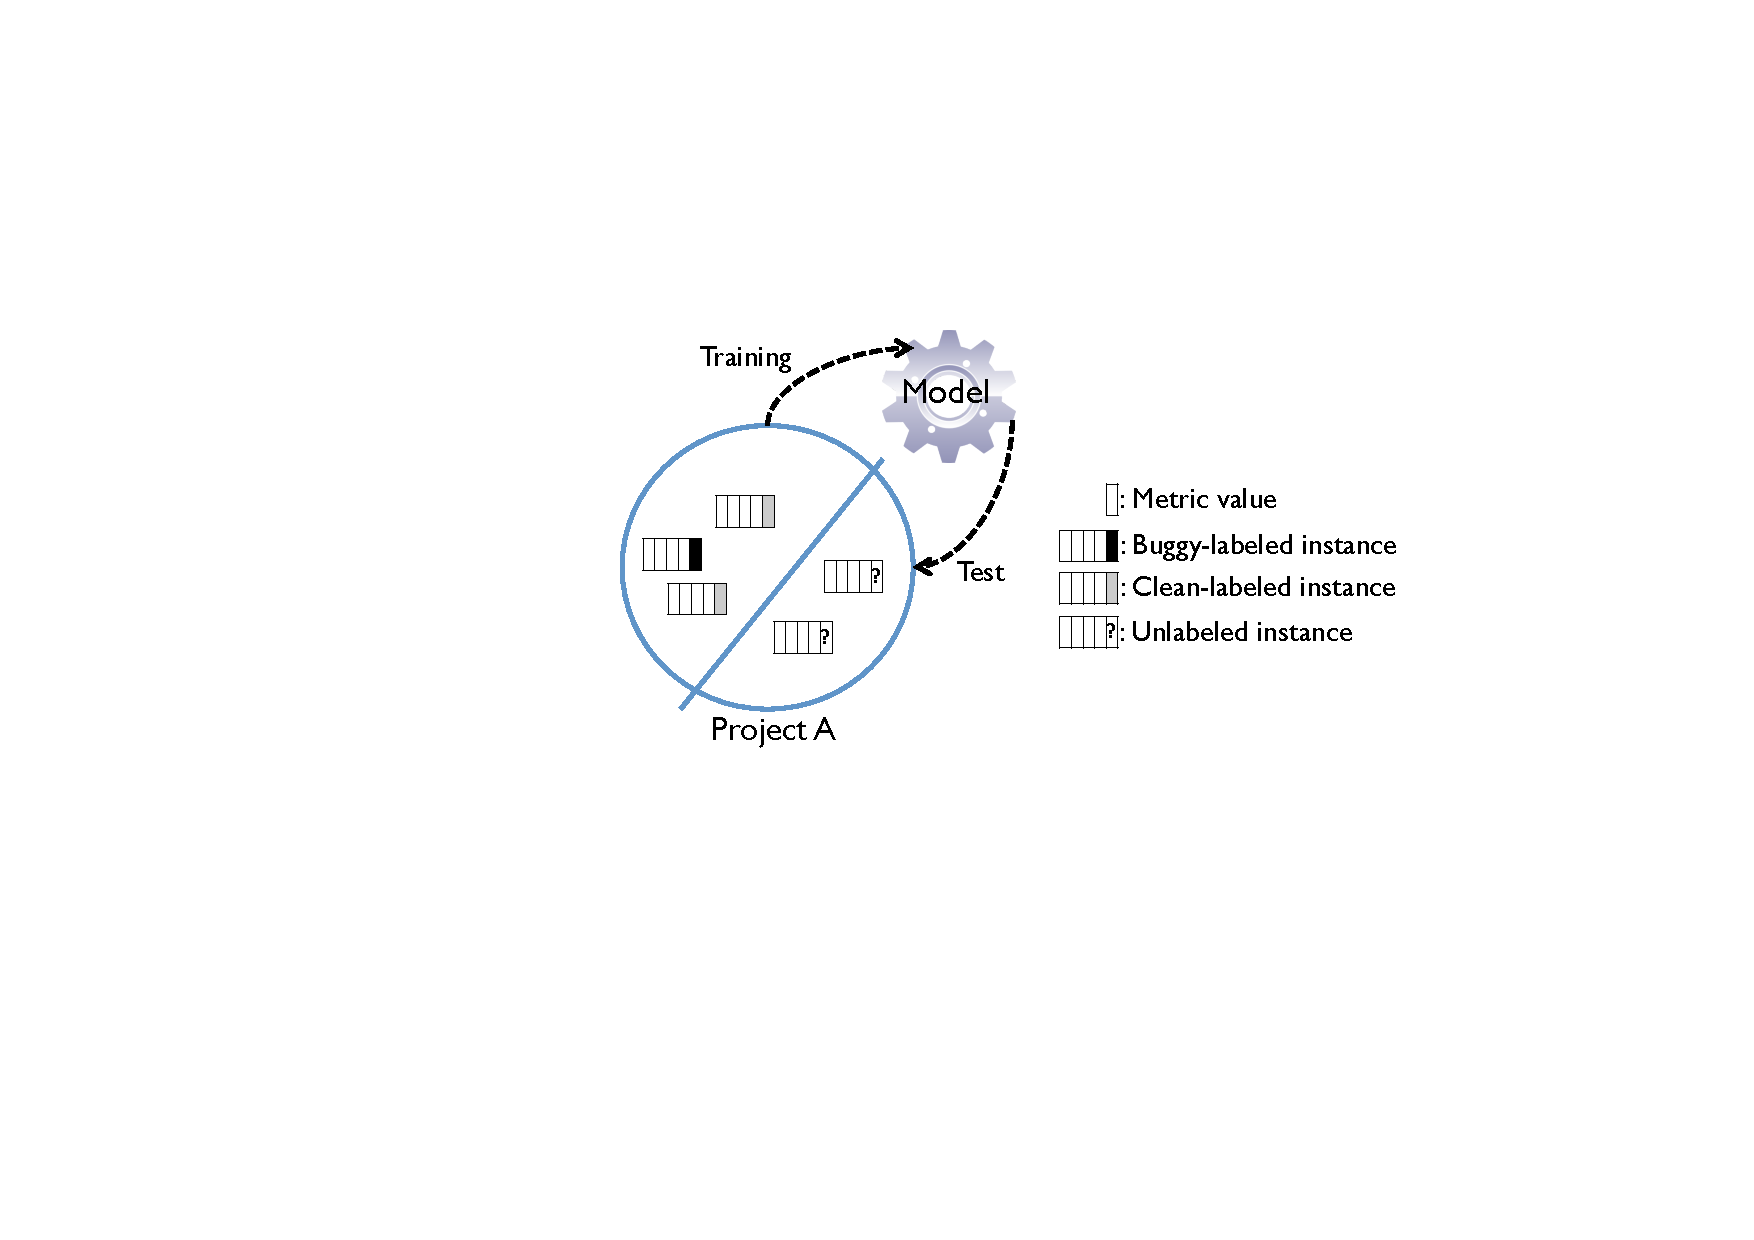
\includegraphics[scale=0.5]{Figures/intro/p_within.pdf}
  	\caption{Within-Project Defect Prediction \tiny{(WPDP)}}
   	\label{fig:subfig1}
 \end{subfigure}
 
 \begin{subfigure}{0.8\linewidth}
 	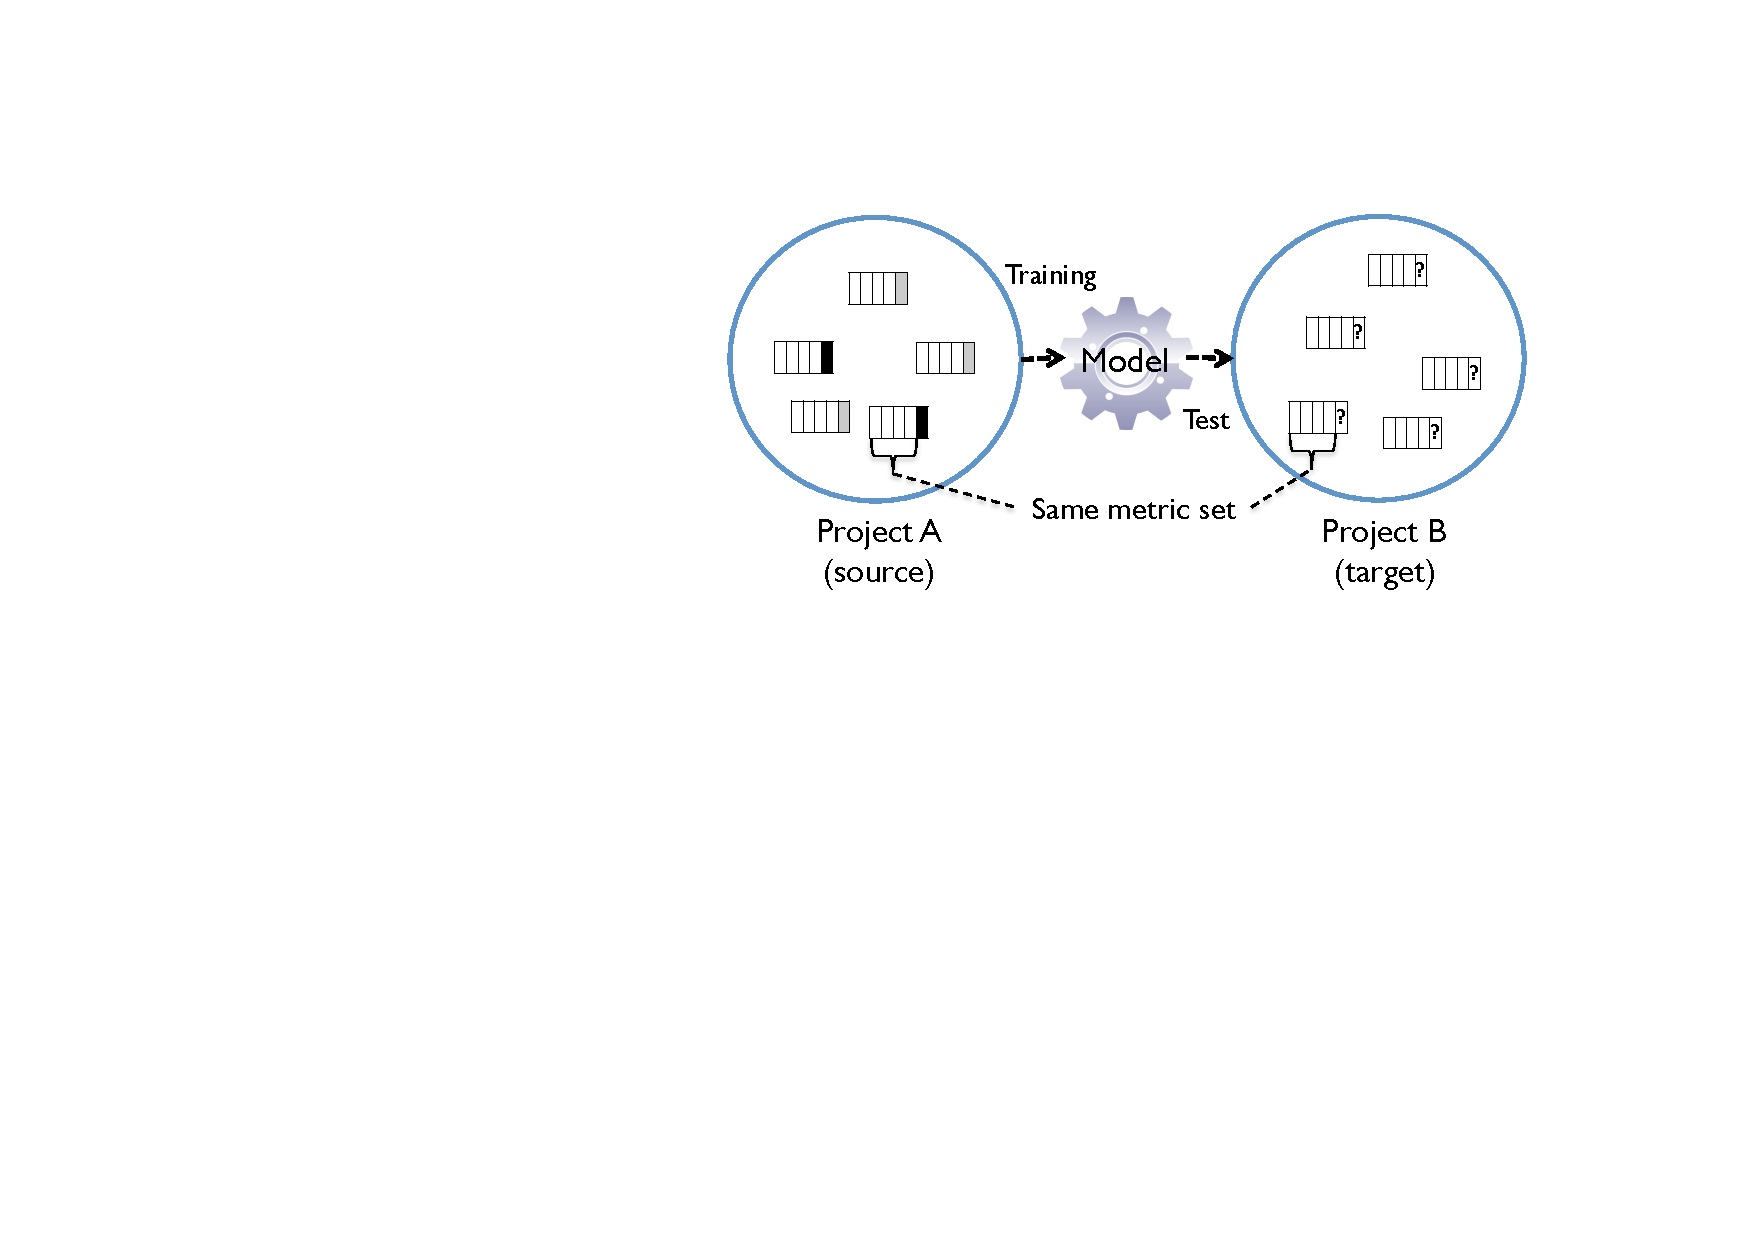
\includegraphics[scale=0.5]{Figures/intro/p_cross.pdf}
  	\caption{Cross-Project Defect Prediction \tiny{(CPDP)}}
   	\label{fig:subfig2}
 \end{subfigure}
 
 \begin{subfigure}{0.8\linewidth}
 	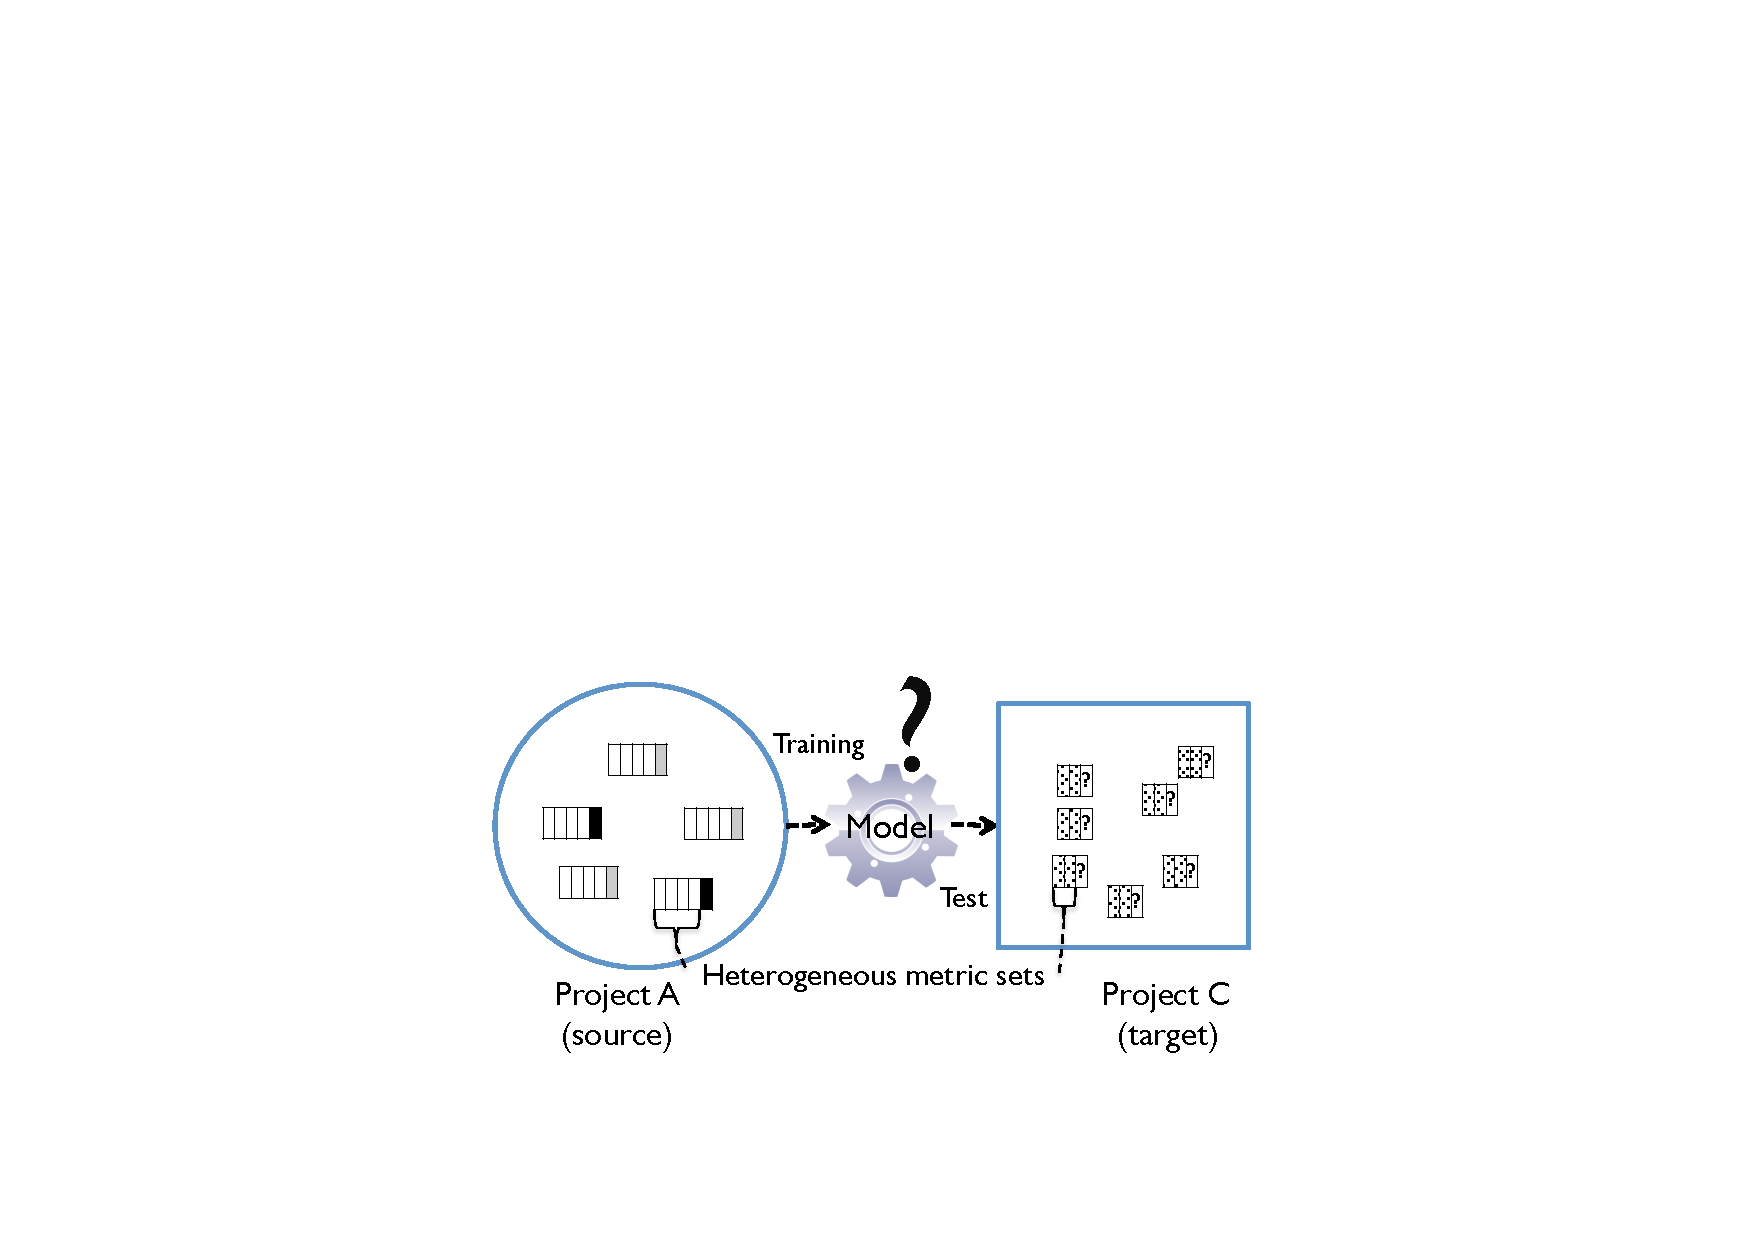
\includegraphics[scale=0.5]{Figures/intro/p_crossdomain.pdf}
  	\caption{Heterogeneous Defect Prediction \tiny{(HDP)}}
   	\label{fig:subfig3}
 \end{subfigure}
 
 \label{fig:type_of_predictions}
 \caption{%
  %Caption of subfigures \subref{fig:subfig1}, 
  %\subref{fig:subfig2} and \subref{fig:subfig3}
  Various Defect Prediction Scenarios
  }
\end{figure}

\subsection{Research Questions}
To systematically evaluate HDP models, we set
two research questions.
\squishlist
  \item RQ1: Is heterogeneous defect prediction comparable to WPDP and existing CPDP approaches for heterogeneous metric sets?
   \item RQ2: What are the  lower  bounds  of  the  size  of source and target  datasets  for  effective HDP?
%   \item[RQ2:] Are cross-domain defect predictions from non-defect to
%   defect datasets comparable to within-predictions?
%  \item[RQ3:] What is the prediction coverage of cross-domain defect
%  prediction?
\squishend
% 
% Since we designed four feature matching analyzers, we identify the
% best co-occurrence analyzers among the five analyzers introduced in
% Section~\ref{sec:analyzers} (RQ1).

\subsection{Contributions}
Our experimental results on RQ1 (in Section~6) shows that HDP models are feasible and their prediction
performance is promising. About 50\% -- 74\% of HDP predictions
are better or comparable to predictions in baseline approaches with statistical
significance.
 
A natural response to the RQ1 results is to ask RQ2; i.e. how early is such transfer
feasible?  Section~7 shown some curious empirical results (from our
work, as well as prior work by researchers in medicine) that show a few hundred examples are enough-- this result is curious since we would have thought that
heterogeneous transfer would complicate move information across projects;
thus {\em increasing} the quantity of data needed for effective transfer.

The results of Section~7 are so curious that is natural to ask are they just a quirk of our data, or do they represent a more general case? To answer this question, and to assess the external validity of the Section~7 results, Section~8 of this paper builds and explores a mathematical model of defect prediction.
That analysis concludes that the Section~7 are actually representive of the general case; i.e. transfer should be possible after a mere few hundred examples. 


% To our knowledge, this is a first study on defect prediction using
% datasets with different feature spaces. We hope this study will suggest a
% promising next step for defect prediction research.

Our contributions are summarized as follows:
\squishlist
  \item Proposing the heterogeneous defect prediction models.
  \item Conducting extensive and large-scale experiments to evaluate
  the heterogeneous defect prediction models.
  \item Empirically validating the lower bounds of the size of source and target datasets for effective heterogeneous defect prediction.
  \item Theoretically demonstrating that the above empirical results are actually
  the general and expected results.
\squishend


\subsection{Extensions from Prior Publication}

We extend the previous conference paper of the same name~\cite{Nam15HDP} in the following ways. First, we motivate this study in the view of transfer learning in software engineering (SE). Thus, we discuss how transfer learning can be helpful to understand the nature of generality in SE and why we focus on defect prediction in terms of transfer learning (Section~\ref{sec:Motivation}). Second, we address new research question about the effective sizes of source and target datasets when conducting HDP.  In Section~\ref{sec:sizelimit} and~\ref{sect:xplain}, we show experimental and theoretical validation to investigate the effective sizes of project datasets for HDP. Third, we discuss more related work with recent studies. In Section~\ref{sec:Background}, we discuss metric sets used in CPDP and how our HDP is similar to and different from recent studies about CPDP using heterogeneous metric sets.
%Fourth, we conduct the effect size analysis using Cliff's $\delta$ to investigate the magnitude of performance improvement by HDP in Section~\ref{sec:Result}.

% This paper is organized as follows. Section~\ref{sec:Background} explains
% the background of our study. % for our framework for cross-domain defect
% % prediction.
% Section~\ref{sec:Approach} presents our HDP model in detail.
% Section~\ref{sec:Evaluation} describes the design of our empirical study. Our
% evaluation results are reported in Section~\ref{sec:Result}. In
% Section~\ref{sec:Discussion}, we discuss insights of our results as well as
% threats to validity. Section~\ref{sec:Conclusion} summarizes and concludes our
% study.



\section{Related Work}
\label{sec:Background}
%\subsection{Cross-project Defect Prediction}
The CPDP approaches have been studied by many researchers
of late~\cite{Canfora13,Ma12,Nam13,Panichella14,Rahman12,Ryu14,Ryu15,Turhan09,Zhang15,Zimmermann09}. Since the performance
of CPDP is usually very poor~\cite{Zimmermann09}, researchers have proposed various techniques to
improve CPDP~\cite{Canfora13,Ma12,Nam13,Panichella14,Ryu14,Ryu15,Turhan09,Watanabe08}. In this section, we discuss CPDP studies in terms of metric sets.

% In the previous studies, cross-prediction was
% applied on datasets with the same metric set or researchers simply used
% following ways to overcome the limitation about different metric sets:
% % ~\sung{I think you need to organize previous work based on this. 
% % Say, A did something. B did something. However, they applied on datasets with the same metric sets.
% % C did something. D did something. Howerver, they used common metric among existing project datasets.
% % \ldots
% % } 
% \squishlist
% 	\item Collecting the same metric set for projects used in an empirical study.
% 	\item Using common metrics among existing project datasets.
% 	\item Conducting cross-prediction within a project group consisting of
% 	existing projects having the same metric set.
% \squishend
  
\subsection{CPDP Using Same/common Metric Sets}
Watanabe et al. proposed the metric compensation approach for
CPDP~\cite{Watanabe08}. The metric compensation transforms a target dataset
similar to a source dataset by using the average metric
values~\cite{Watanabe08}.
To evaluate the performance of the metric compensation, Watanabe et al. collected
two defect datasets with the same metric set (8 object-oriented
metrics) from two software projects and then conducted
CPDP~\cite{Watanabe08}.

Rahman et al. evaluated the CPDP performance in terms of
cost-effectiveness and confirmed that the prediction performance of CPDP is
comparable to WPDP~\cite{Rahman12}. For the empirical study, Rahman et al.
collected 9 datasets with the same process metric set~\cite{Rahman12}.

Fukushima et al. conducted an empirical study of just-in-time defect prediction
in the CPDP setting~\cite{Fukushima14}. They used 16
datasets with the same metric set~\cite{Fukushima14}. The 11 datasets were
provided by Kamei et al. but 5 projects were newly collected with the same metric
set of the 11 datasets~\cite{Fukushima14,Kamei13}.

However, collecting datasets with the
same metric set might limit CPDP. For example, if
existing defect datasets contain object-oriented metrics such as CK
metrics~\cite{Basili96}, collecting the same object-oriented metrics is
impossible for projects that are written in non-object-oriented languages.

Turhan et al. proposed the nearest-neighbour (NN) filter to improve the
performance of CPDP~\cite{Turhan09}. The basic idea of the NN
filter is that prediction models are built by source instances that are
nearest-neighbours of target instances~\cite{Turhan09}. To conduct
CPDP, Turhan et al. used 10 NASA and SOFTLAB datasets in the
PROMISE repository~\cite{promise12,Turhan09}.
%With the NN filter, cross-prediction results improved from 0.26 to 0.35 in
%terms of average f-measure. However, within-prediction results were still the
% best (0.37)~\cite{Turhan09}.

Ma et al. proposed Transfer Naive Bayes (TNB)~\cite{Ma12}. The TNB builds a
prediction model by weighting source instances similar to target
instances~\cite{Ma12}. Using the same datasets used by Turhan et al., Ma et al.
evaluated the TNB models for CPDP~\cite{Ma12,Turhan09}.
% The cross-prediction performance of TNB
% (0.39) outperformed that of the NN filter (0.35) in terms of average f-measure~\cite{Ma12}.

Since the datasets used in the empirical studies of Turhan et al. and Ma et al.
have heterogeneous metric sets, they conducted CPDP using the common
metrics~\cite{Ma12,Turhan09}. There is another CPDP study with the top-K
common metric subset~\cite{He14subset}. However, as explained in
Section~\ref{sec:Introduction}, CPDP using common metrics is
worse than WPDP~\cite{He14subset,Turhan09}.
%   The NASA and SOFTLAB datasets have different
% metric sets (21 to 39 metrics)~\cite{Turhan09}. Among them, only 17 common
% metrics were used in their empirical studies.



Nam et al. adapted a state-of-the-art
transfer learning technique called Transfer Component Analysis (TCA) and
proposed TCA+~\cite{Nam13}. They used 8
datasets in two groups, ReLink and AEEEM, with 26 and 61 metrics
respectively~\cite{Nam13}.
% 
% He et al. conducted the empirical study for defect prediction
% using a simplified metric set~\cite{He14subset}. They conducted CPDP on 34
% datasets with the same metric set (20 code metrics) and showed CPDP

However, Nam et al. could not conduct CPDP between ReLink and AEEEM because they
have heterogeneous metric sets.
Since the project pool with the same metric set is very limited, conducting
CPDP using a project group with the same metric set can be
limited as well. For example, at most 18\% of defect datasets in the
PROMISE repository have the same metric set~\cite{promise12}. In other words,
we cannot directly conduct CPDP for the 18\% of the defect datasets by
using the remaining (82\%) datasets in the PROMISE
repository~\cite{promise12}.


There are recent CPDP studies using datasets with the same metric sets or using common metric sets~\cite{Canfora13,promise12,Panichella14,Zhang15,Ryu14,Ryu15}.
%Panichella. Canfora Ryu, Zhang(comsac)
Canfora et al., Panichella et al., and Zhang et al.
used ten Java projects only with the same metric set from the PROMISE
repository~\cite{Canfora13,promise12,Panichella14,Zhang15}.
Ryu et al. proposed the value-cognitive boosting and transfer cost-sensitive boosting approaches for CPDP~\cite{Ryu14,Ryu15}. Ryu et al. used common metrics in NASA and SOFTLAB datasets~\cite{Ryu14} or Jureczko datasets with the same metric set from the PROMISE repository~\cite{Ryu15}. These recent studies for CPDP did not discuss about the heterogeneity of metrics across project datasets.
% ~\sung{say how many \% of PROMISE projects have the same dataset.}
% although there are lots of existing datasets available.

% Cross-prediction with TCA+ showed comparable results to within-prediction in average f-measure on 8 open source projects~\cite{Nam13}.

% Fukushima et al. conducted an empirical study of just-in-time defect prediction
% under cross-project settings on 11 open source projects with the same metric set~\cite{Fukushima14}. 
% They observed cross-prediction models can be
% improved in terms of AUC by selecting a source dataset similar to a target
% dataset~\cite{Fukushima14}.


Zhang et al. proposed the universal model for CPDP~\cite{Zhang14}.
%Since the individual project may have its specific
%defect characteristic, the universal model may not work for all
%projects~\cite{Zhang14}. To resolve this limitation, Zhang et al. proposed
%context-aware rank transformations that change metric values ranged from 1 to
% 10 across all projects~\cite{Zhang14}. In this way, 
The universal model is
built using 1398 projects from SourceForge and Google code and leads to
comparable prediction results to WPDP in their experimental
setting~\cite{Zhang14}.

However, the universal defect prediction model may be difficult to apply for the
projects with heterogeneous metric sets since the universal
model uses 26 metrics including code metrics, object-oriented metrics, and
process metrics. In other words, the model can only be applicable for
target datasets with the same 26 metrics. In the case where the target project
has not been developed in object-oriented languages, a universal model built
using object-oriented metrics cannot be used for the target dataset.
%  or need to costly build a new universal model with the same
% metric set of the target dataset.

\subsection{CPDP Using Heterogeneous Metric Sets}
He et al. addressed the limitations due to
heterogeneous metric sets in CPDP studies listed
above~\cite{He14}.
Their approach, CPDP-IFS, used distribution
characteristic vectors of an instance as metrics.
The prediction performance of their best approach is comparable to or
helpful in improving regular CPDP models~\cite{He14}.

However, the approach by He et al. is not compared with WPDP~\cite{He14}.
Although their best approach is helpful to improve regular CPDP models, the
evaluation might be weak since the prediction performance of a regular CPDP is
usually very poor~\cite{Zimmermann09}. In addition, He et al. conducted
experiments on only 11 projects in 3 dataset groups~\cite{He14}.

Jing et al. proposed heterogeneous cross-company defect prediction based on the extended canonical correlation analysis (CCA+)~\cite{Jing15} to address the limitations of heterogeneous metric sets. Their approach adds dummy metrics with zero values for non-existing metrics in source or target datasets and then transforms both source and target datasets to make their distributions similar. CCA+ was evaluated on 14 projects in four dataset groups.
%One of issues of CCA+ is that it was not properly evaluated on cross-company dataset groups. For example, ReLink datasets are not from the same company but they just have same metric sets.

% In our previous study, we used two groups of datasets, ReLink and
% AEEEM~\cite{Nam13}. 
We propose HDP to address the above
limitations caused by projects with heterogeneous metric sets.
Contrary to the study by He et al.~\cite{He14}, we compare HDP to
WPDP, and HDP achieved better or comparable prediction performance to WPDP in
about 68\% of predictions.
Comparing to the experiments for CCA+~\cite{Jing15} on 14 projects, we conducted more extensive experiments on 28 projects in 5 dataset groups. In addition, CCA+ transforms original source and target datasets so that it is difficult to directly explain the meaning of metric values generated by CCA+~\cite{Jing15}. However, HDP keeps the original metrics and builds models with the small subset of selected and matched metrics between source and target datasets in that it can make prediction models simpler and easier to explain~\cite{Nam15HDP,Shihab14}. In
Section~\ref{sec:Approach}, we explain our approach in detail.

% In this section, we explain transfer learning on different domains.
% Transfer learning is one of the recent very active research topics in the
% machine learning community~\cite{Pan10}. Transfer learning can reduce expensive
% costs incurred while collecting and labeling training data by transferring
% knowledge from existing data and models~\cite{Pan10}.
% 
% To define transfer learning formally, Pan et al. gave the definition of a
% domain; ``a domain, $D$, consists of two components: a feature space $\chi$ and
% a marginal distribution $P(X)$, where $X=\{x_1,...,x_n\}\in
% \chi$''~\cite{Pan10}. According to this definition, a domain can be
% represented as follows: $D=\{\chi,P(X)\}$. When we say two domains are different, it
% represents different feature spaces, $\chi$, or different distributions, $P(X)$.
% 
% Most transfer learning studies focused on different distributions by
% assuming feature spaces are the same across datasets, but less focused on
% different feature spaces~\cite{Pan10}.
% Since our study aims to resolve the issue on defect prediction on
% datasets with different feature spaces, the term `different
% domains' stands for `different feature spaces of datasets' throughout the paper.
% 
% 
% Dai et al.~\cite{Dai08} proposed Translated Learning to address transfer
% learning on different feature spaces.
% The core approach used in translated learning is to identify co-occurrence features, which are
% linked between source and target features to migrate knowledge of source data to
% models for target data~\cite{Dai08}. Yang et al.~\cite{Yang09} introduced
% heterogeneous transfer learning for image clustering by using text
% data, which have a different feature space to image data. Zhu et
% al.~\cite{Zhu11} proposed heterogeneous transfer learning for image
% classification using text data that has different feature spaces. However, all
% these studies utilize tags given to images on web sites to link/bridge difference feature sets so that it is
% difficult to directly apply their approaches for our cross-domain defect
% prediction.
% % Translated learning is an independent
% % algorithm from existing machine learning algorithms such as Decision tree,
% % Random Forest, Logistic Regression and etc., which are widely used for defect prediction.
% 
% Inspired by translated and heterogeneous transfer learning, we design
% our approaches to identify co-occurrence features between source and target
% datasets for the cross-domain defect prediction. Our approaches are based on
% statistical information and existing approaches that might be used to measure
% similarity between two features.
% %working together with
% %existing machine learning algorithms for defect prediction.
% In Section~\ref{sec:analyzers}, we describe in detail how to identify
% co-occurrence features for our cross-domain defect prediction.


% \subsubsection{Random Analyzer}
% We defined random analyzer, where we match srouce and target feautres randomly
% to evaluate if the proposed analyzers work better than the random analyzer.


%
\section{Motivation}
\label{sec:Motivation}

\subsection{Why Explore Transfer Learning?}
One reason to explore transfer learning
is to study the nature of
generality in SE. Professional
societies assume such generalities exist when they
offer lists of supposedly general ``best practices'':
\squishlist
\item For example, the  IEEE 1012 standard for software
  verification~\cite{1012} proposes numerous methods for assessing software quality;
\item
 Endres and Rombach catalog
dozens of lessons of software
engineering~\cite{endres03} such as McCabe's Law (functions with a ``cyclomatic complexity'' greater
than ten are more error prone);
\item Further, many other
widely-cited researchers do the same such as Jones~\cite{jones10} and
Glass~\cite{glass02} who list (for exmple)
Brooks' Law (adding programmers to a late project makes it later).
% Boehm~\cite{hoehm00b}.
\item
  More generally, Budgen and Kitchenham seek to
reorganize SE research using general conclusions
drawn from a larger number of
studies~\cite{budgen06,budgen09}.
\squishend

Given the constant pace of change within SE, can we trust
those supposed generalities?
Numerous {\em local learning} results show that we
should mistrust general conclusions (made over a
wide population of projects) since they may not hold
for projects~\cite{me12d,betten14}. Posnett et al.~\cite{posnett11}
discuss {\em ecological inference} in software
engineering, which is the concept that what holds
for the entire population also holds for each
individual. They learn models at different levels
of aggregation (modules, packages, and files) and show
that models working at one level of aggregation
can be sub-optimal at others.  For example, Yang et
al.~\cite{yang11}, Bettenburg et
al.~\cite{betten14}, and Menzies et al.~\cite{me12d}
all explore the generation of models using {\em all}
data versus {\em local} samples that are more specific
to particular test cases. These papers report that
better models (sometimes with much lower variance in
their predictions) are generated from local
information.
These results have an unsettling effect on anyone
struggling to propose policies for an organization.
If all prior conclusions can change for the new
project, or some small part of a project, how can
any manager ever hope to propose and defend IT
policies (e.g., when should some module be inspected,
when should it be refactored, where to focus
expensive testing procedures, etc.)?

If we cannot {\em generalize} to all projects and all parts
of current projects, perhaps a more achievable goal is to {\em stabilize} the pace of conclusion change.
While it may be
a fool's errand and wait for eternal and global SE
conclusions, one possible approach is for organizations
to declare $N$ prior projects as {\em reference projects},
from which lessons learned will be transferred to new projects.
In practice, using such reference sets requires three processes:
\begin{enumerate}
\item Finding the reference sets (this paper shows that finding
  them may not require extensive and protracted data collection, at least for defect prediction).
  \item Recognizing when to update the reference set. In practice,
  this could be as simple as noting when predictions start failing for new projects---at which time, we would loop to the point 1).
\item Transferring
  lessons from the reference set to new projects.
\end{enumerate}
In the case where all the datasets use the same metrics, this is a relatively
simple task. Krishna et al.~\cite{krishna16} have found such reference projects just by training of
a project X then testing on a project Y (and the reference set are the project Xs with highest scores).
Once found, these reference sets can generate policies of an organization that are
stable just as long as the reference set is not updated.

In this paper, we do not address the pace of change in the reference set
(that is left for future work).
Rather, we focus on the point 3): transferring lessons from
the reference set to new projects in the case of heterogeneous data sets. To support this third point,
we need to resolve the problem
  that this paper addresses, i.e., data expressed in different terminology
  cannot transfer till there is enough data to match old projects to new projects.




\subsection{Why Explore Defect Prediction?}

There are many lessons we {\em might} try to transfer between projects
about staffing policies, testing methods, language choices, etc. While
all those matters are important and are worthy of research, this section
discusses why we focus on defect prediction.

Human programmers are clever, but flawed. Coding  adds functionality, but also defects.
Hence, software sometimes crashes (perhaps at the most awkward or dangerous moment) or delivers
the wrong functionality. For a very long list of software-related errors,
see  Peter Neumann's ``Risk Digest'' at http://catless.ncl.ac.uk/Risks.

Since programming inherently
introduces defects into  programs, it is important to test them before they're used.
Testing is expensive.
Software assessment budgets are finite
while assessment effectiveness increases
exponentially with assessment effort.
For example, for  black-box testing methods,
a {\em linear} increase
in the confidence $C$ of finding  defects
can take {\em exponentially} more effort.\footnote{A randomly selected
input to a program will find a fault with probability $p$.
After $N$ random black-box tests, the chances of the inputs
not revealing any fault
is $(1-p)^N$. Hence, the chances $C$ of seeing the fault is $1-(1-p)^N$
which can be rearranged to
 $N(C,p)=log(1 -
C)/log(1-p)$. For example, $N(0.90,10^{-3})=2301$
but $N(0.98,10^{-3})=3901$; i.e., nearly double the number of tests.}
Exponential costs quickly exhaust finite resources so
standard practice is to apply the best
available  methods on code sections that seem most critical.
But any method that focuses on parts of the code
can blind us to defects in other areas. Some  {\em lightweight sampling policy} should be used to explore the rest of the system.
This sampling policy will always be incomplete.
Nevertheless, it is the only option when
resources prevent a complete assessment of everything.

One such lightweight sampling policy is defect predictors learned from software metrics such as static code attributes.
For example, given static code descriptors for each module, plus a count of the number of issues raised during inspect (or at runtime),
data miners can learn where the probability of software defects is highest.


The rest of this section argues that such defect predictors are   {\em easy to
use}, {\em widely-used}, and {\em useful} to use.

{\em Easy to use:} Various software metrics such as static code attributes and process metrics can be automatically collected, even for very large systems, from software repositories~\cite{Basili96,Halstead77,McCabe76,nagappan05,Rahman13}.
Other methods, like  manual code reviews, are far slower and far more labor-intensive.
For example, depending on the review methods, 8 to 20 LOC/minute can be
inspected and this effort repeats for all members of the review team,
which can be as large as four or six people~\cite{me02f}.

{\em Widely used:}  Researchers and industrial practitioners  use the software metrics to guide software
quality predictions.
 Defect prediction models have been reported
  at large industrial companies such as Google~\cite{lewis13}, Microsoft~\cite{Nagappan06}, AT\&T~\cite{Ostrand05}, and Samsung~\cite{Kim15remi}.
Verification and validation (V\&V) textbooks
\cite{rakitin01} advise using the software metrics
to decide which modules are worth manual inspections.


{\em Useful:}
Defect predictors often  find the location of  70\% (or more)
of the defects in code~\cite{me07b}.
Defect predictors have some level of generality:
predictors learned at NASA~\cite{me07b} have also been found useful elsewhere
(e.g., in Turkey~\cite{tosun10,tosun09}).
The success of this method in  predictors in finding bugs is markedly
higher than other currently-used
industrial
methods such as manual code reviews. For example,
a  panel at {\em IEEE Metrics
2002}~\cite{shu02} concluded that manual software  reviews can find ${\approx} 60\%$
of defects.
In another work,
Raffo documents the typical defect detection capability of
industrial review methods:   around 50\%
 for full Fagan inspections~\cite{fagan76} to
21\% for less-structured inspections.
In some sense, defect prediction might not be necessary for small software projects.
However, software projects seldom grow by small fractions in practice. For example, a project team may suddenly merge a large branch into a master branch in a version control system or add a large third-part library. In addition, a small project could be just one of many other projects in a software company. In this case, the small project also should be considered for limited resource allocation in terms of software quality control by the company. For this reason, defect prediction could be useful even for the small software projects in practice.

Not only do defect predictors perform well compared to manual methods,
they also are competitive with certain automatic methods.
A recent study at ICSE'14, Rahman et al.~\cite{rahman14:icse} compared
(a) static code analysis tools FindBugs, Jlint, and Pmd and (b) defect predictors
(which they called ``statistical defect prediction'') built using logistic regression.
They found  no significant differences in the cost-effectiveness
of these  approaches. Given this equivalence, it is significant to note that
defect prediction can be quickly adapted to new languages by building lightweight
parsers to extract high-level software metrics. The same is not true for static code analyzers---these need extensive modification before they can be used on new
languages.

Having offered general high-level notes on defect prediction,
the next section describes in detail the related work on this topic.

\section{Approach}
\label{sec:Approach}
% We name our technique for CPDP on datasets having
% different metric sets as ``cross-domain defect prediction.'' In this study, we
% define {\em a domain} as the development environment of a software project. The
% reason for different metric sets is due to different development environment.
% For example, we cannot extract the object-oriented metrics from the software
% projects that are not developed in the object-oriented languages. In addition,
% metric values may have different distributions in different development
% environments. 
% %  In the machine
% % learning literature, ``different domains'' indicate different feature spaces
% In other words, defect prediction datasets collected from different
% projects developed by various development environments can have different metric sets
% and distributions (i.e. different domains)~\cite{promise12}.
% Thus, our proposed approaches focus on resolving
% the differences between projects from the various domains to improve prediction
% performance.

\begin{figure}[t]
	\centering
	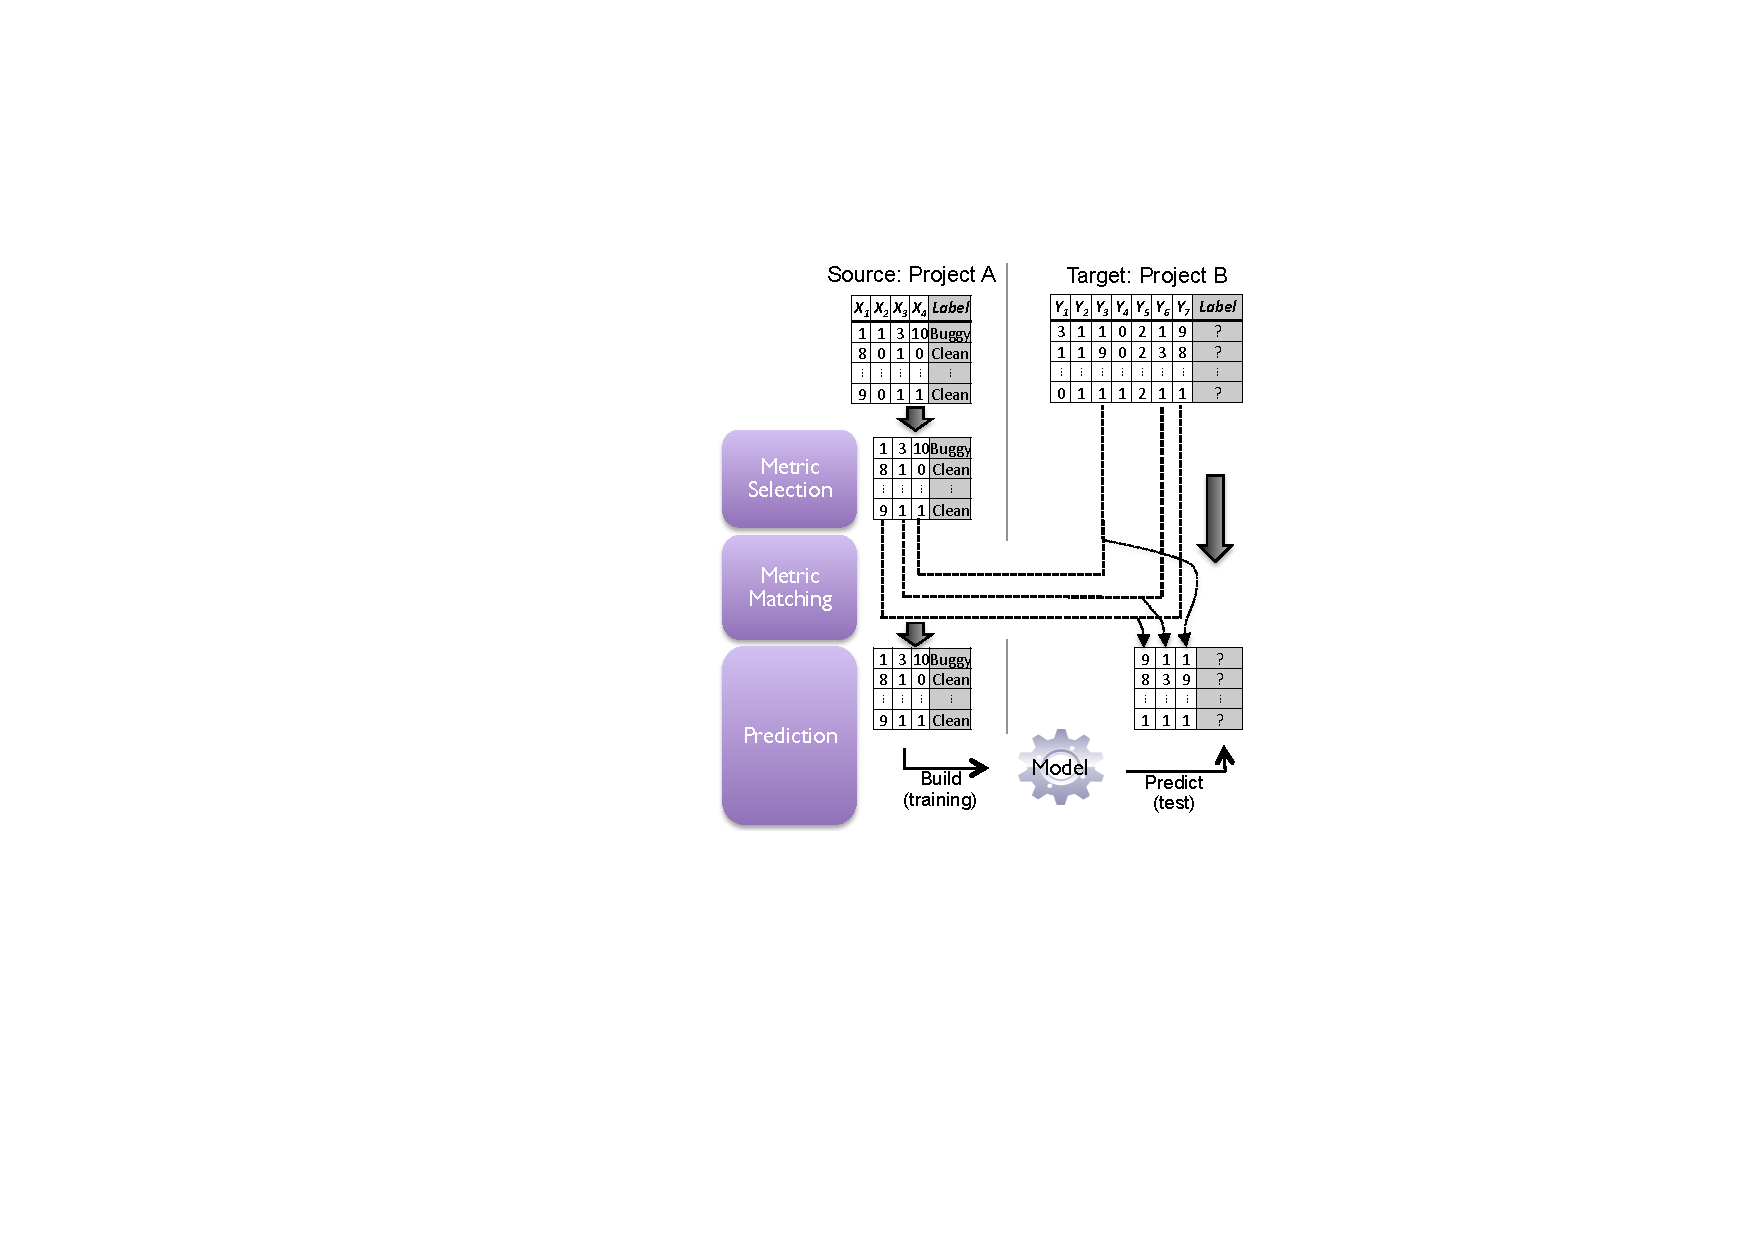
\includegraphics[width=0.925\linewidth]{Figures/framework.pdf}
	\caption{Heterogeneous defect prediction}
	\label{fig:framework}
\end{figure}

Figure~\ref{fig:framework} shows the overview of HDP based on metric selection
and metric matching. In the figure, we have two datasets, Source and Target,
with heterogeneous metric sets. Each row and column of a dataset represents an
instance and a metric, respectively, and the last column represents instance
labels. As shown in the figure, the metric sets in the source and target datasets are not identical ($X_1$ to $X_4$ and $Y_1$ to
$Y_7$ respectively).

When given source and target datasets with heterogeneous metric sets, for metric
selection we first apply a feature selection technique to the source. Feature
selection is a common approach used in machine learning for selecting a subset
of features by removing redundant and irrelevant features~\cite{Guyon03}.
% Since
% software metrics can be considered as features in the machine learning sense,
%by using feature selection techniques.
% As discussed in Section~\ref{sec:Background}, using only common metrics between
% source and target defect datasets to build a prediction model limits the
% prediction performance since informative metrics may not be included in the
% common metric set. To address this issue, 
We apply widely used feature selection
techniques for metric selection of a source dataset as in
Section~\ref{sec:metricselection}~\cite{Gao11,Shivaji13}.
% In addition, applying
%feature selection can be helpful to build a better defect prediction
%model~\cite{Shivaji13,Catal09,CHALLAGULLA08}.

After that, metrics based on their similarity such as distribution
or correlation between the source and target metrics are matched up. In
Figure~\ref{fig:framework}, three target metrics are matched with the
same number of source metrics.

After these processes, we finally
arrive at a matched source and target metric set. With the final
source dataset, HDP builds a model and predicts labels of
target instances.

In the following subsections, we explain the metric selection and matching in
detail.
  
%   \item {\bf Filtering out source features whose median value of buggy
%   instances are lower than that of clean instances}: The intuition of this
%   strategy is based on the unique characteristic of defect prediction datasets,
%   i.e. defect prediction metrics are positively correlated. In other
%   words, typical defect prediction metrics (features) measure the complexity of
%   the source code and development process so that there is a tendency that
%   {\em a higher complexity causes more
%   bug-proneness}~\cite{DAmbros12,Menzies08,Rahman13}. For example, if a
%   source code file has more {\em LOC}, one of complexity measures, then the file may have a higher chance
%   of being bug-prone. This is a typical rationale for defect prediction metrics.
%   However, some features in datasets may not follow this rationale; the lower
%   feature (metric) value, the higher bug-proneness. We regard them as noisy
%   features.~\sung{I don't agree with this. As long as they are correlated it
% is fine. For example, \# of comments. Say more comments leads to less bugs.
% But it's OK. Perhaps, what you did here is another feature selection? You remove non positively correlated features? What would be the results without this process?} Thus, to filter out noisy features, we remove source features whose   median value is lower than that of clean instances. In   Section~\ref{sec:filter}, we describe how to filter out these noisy features
%   in detail.
% \squishend


% Figure~\ref{fig:framework} gives the cross-domain defect
% prediction overview.
% The cross-domain defect prediction consists of four components: label adjuster,
% feature selector, co-occurrence analyzer, and cross-prediction runner.
% 
% The label adjuster makes label names between source and target datasets the same
% if they are different. For example, NASA and SOFTLAB defect datasets in the PROMISE
% repository have different buggy (clean) labels, that is, ``Y'' (``N'') and
% ``true'' (``false''), respectively~\cite{promise12}. We convert these different
% label values; ``Y'' and ``true'' as ``buggy'' and ``N'' and ``false'' as ``clean''.

\subsection{Metric Selection in Source Datasets}\label{sect:fss}
\label{sec:metricselection}
For metric selection, we used various feature selection
approaches widely used in defect prediction such as gain ratio, chi-square,
relief-F, and significance attribute evaluation~\cite{Gao11,Shivaji13}.
According to benchmark studies about various feature selection approaches, a
single best feature selection approach for all prediction models does not
exist~\cite{Catal09,Hall03,Liu02}. For this reason, we conduct experiments
under different feature selection approaches. When applying feature selection
approaches, we select top 15\% of metrics as suggested by Gao et
al.~\cite{Gao11}. In addition, we compare the prediction results with or without
metric selection in the experiments.

% The key idea of CFS
%is to select features that highly correlate with class labels but not correlate
% with other features within the same dataset~\cite{Hall98}.  However, we chose CFS since it is fast and widely used in benchmark
%studies~\cite{Menzies07,Catal09,Hall03,Liu02,CHALLAGULLA08}.
%  Hall
% proposed the CfsSubsetEval algorithm by combining a correlation measure and a heuristic
% search technique~\cite{Hall98}.



% It is possible to use other feature selection
% approaches~\cite{Shivaji13}. However, we used the CfsSubsetEval in our
% experimental setting for easy replication since 
% the CfsSubsetEval is a Weka's default feature selection
% algorithm~\cite{Weka}.~\sung{This is very weak argument. As long as other algorithms are available, they can replicate. Provide other reasons. Perhaps, this algorithm is simple?fast? many others are using this?}

\subsection{Matching Source and Target Metrics}
%  based on
% distribution similarity}
\label{sec:analyzers}

To match source and target metrics, we measure the similarity of each source and
target metric pair by using several existing methods such as percentiles,
Kolmogorov-Smirnov Test, and Spearman's correlation
coefficient~\cite{Massey51,Spearman10}.
We define the following three analyzers
for metric matching:
\vspace{-0.2em}
\squishlist
	\item Percentile based matching (PAnalyzer)
	\item Kolmogorov-Smirnov Test based matching (KSAnalyzer)
	\item Spearman's correlation based matching (SCoAnalyzer)
	%\item Popularity index based matching (PiAnalyzer)
\squishend

% \begin{figure}[t]
% 	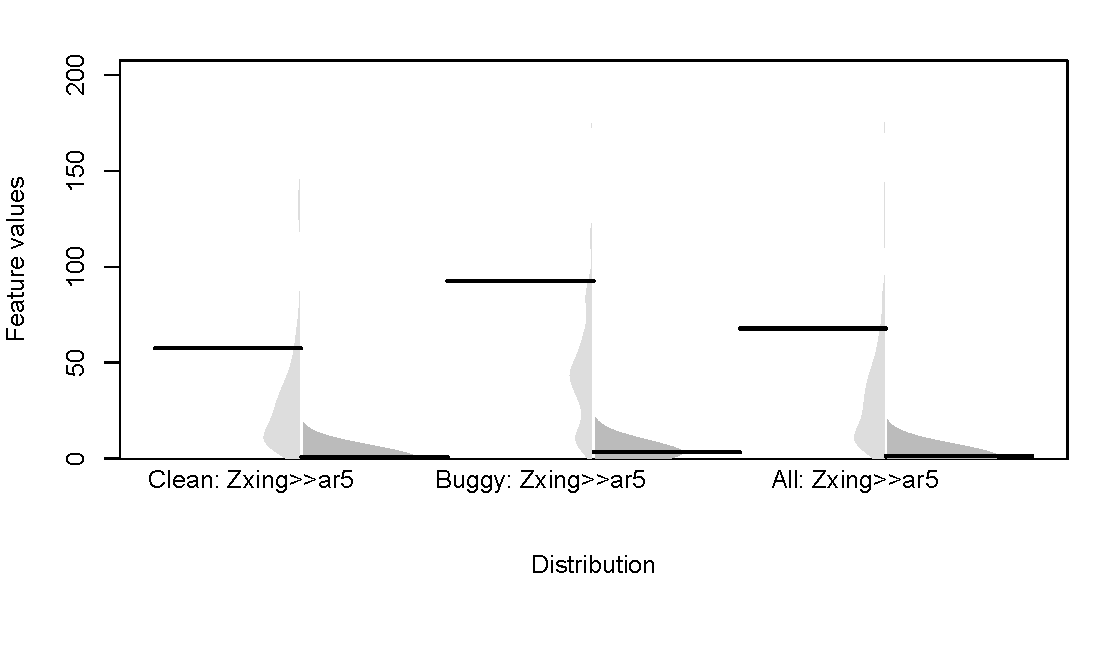
\includegraphics[width=\linewidth]{Figures/Result/beanplot_manual_matching.pdf}
% 	\caption{Feature value distribution of a common feature, `{\em lines of code
% 	and comments}', between datasets, Zxing and ar5. The three plots shows feature
% 	value distributions for clean, buggy, and all instances respectively. A solid
% 	horizontal line represents an average feature value for each plot.}
% 	\label{fig:common_feature}
% \end{figure}
% 
% % To build efficient machine learning models, the distribution of both
% %   training and test data should be same~\cite{Pan10}.However,
% %   datasets from different domains most likely have different distributions.
% 
% Since researchers in previous studies of cross-project defect prediction focused
% on making different features similar or selecting similar instances, similarity
% between source and target datasets is an important factor for
% cross-prediction~\cite{Nam13,Ma12,Turhan09,Watanabe08}. How
% Figure~\ref{fig:common_feature} shows distributions of a feature, `{\em lines of code and comments}', in two datasets, Zxing and ar5. In the figure, the light grey areas represent the feature value distribution of Zxing and the dark
% grey areas are for ar5. Three sets of plots show feature distributions of clean,
% buggy, and all (both buggy and clean) instances. As in
% Figure~\ref{fig:common_feature}, feature distributions between Zxing and ar5 are
% very different although it is the same metric, `{\em lines of code and
% comments}'. For this reason, we avoid using common features between two datasets.
% Instead, we just match features between
% source and target datasets based on their similarities, and the
% matched features for defect prediction.
% In Section~\ref{sec:analyzers}, we explain four
% feature matching approaches.
% \item 

%\subsection{Cross-domain Defect Prediction Model}
%\label{sec:framework}


% In case that a dataset
% has nominal, ordinal, or cardinal values as labels, we should transform the
% values into binary class labels. For example, if a dataset have ten cardinal
% label values from 1 to 10, we can set a cutoff value for a buggy label. Assuming
% the cutoff value for a buggy label is 5, we can label instances with the values
% below 5 or same as 5 as buggy, otherwise as clean.
% Label adjusting is a very preliminary step to build a cross-domain prediction
% model.

\begin{figure}[t]
	\centering
	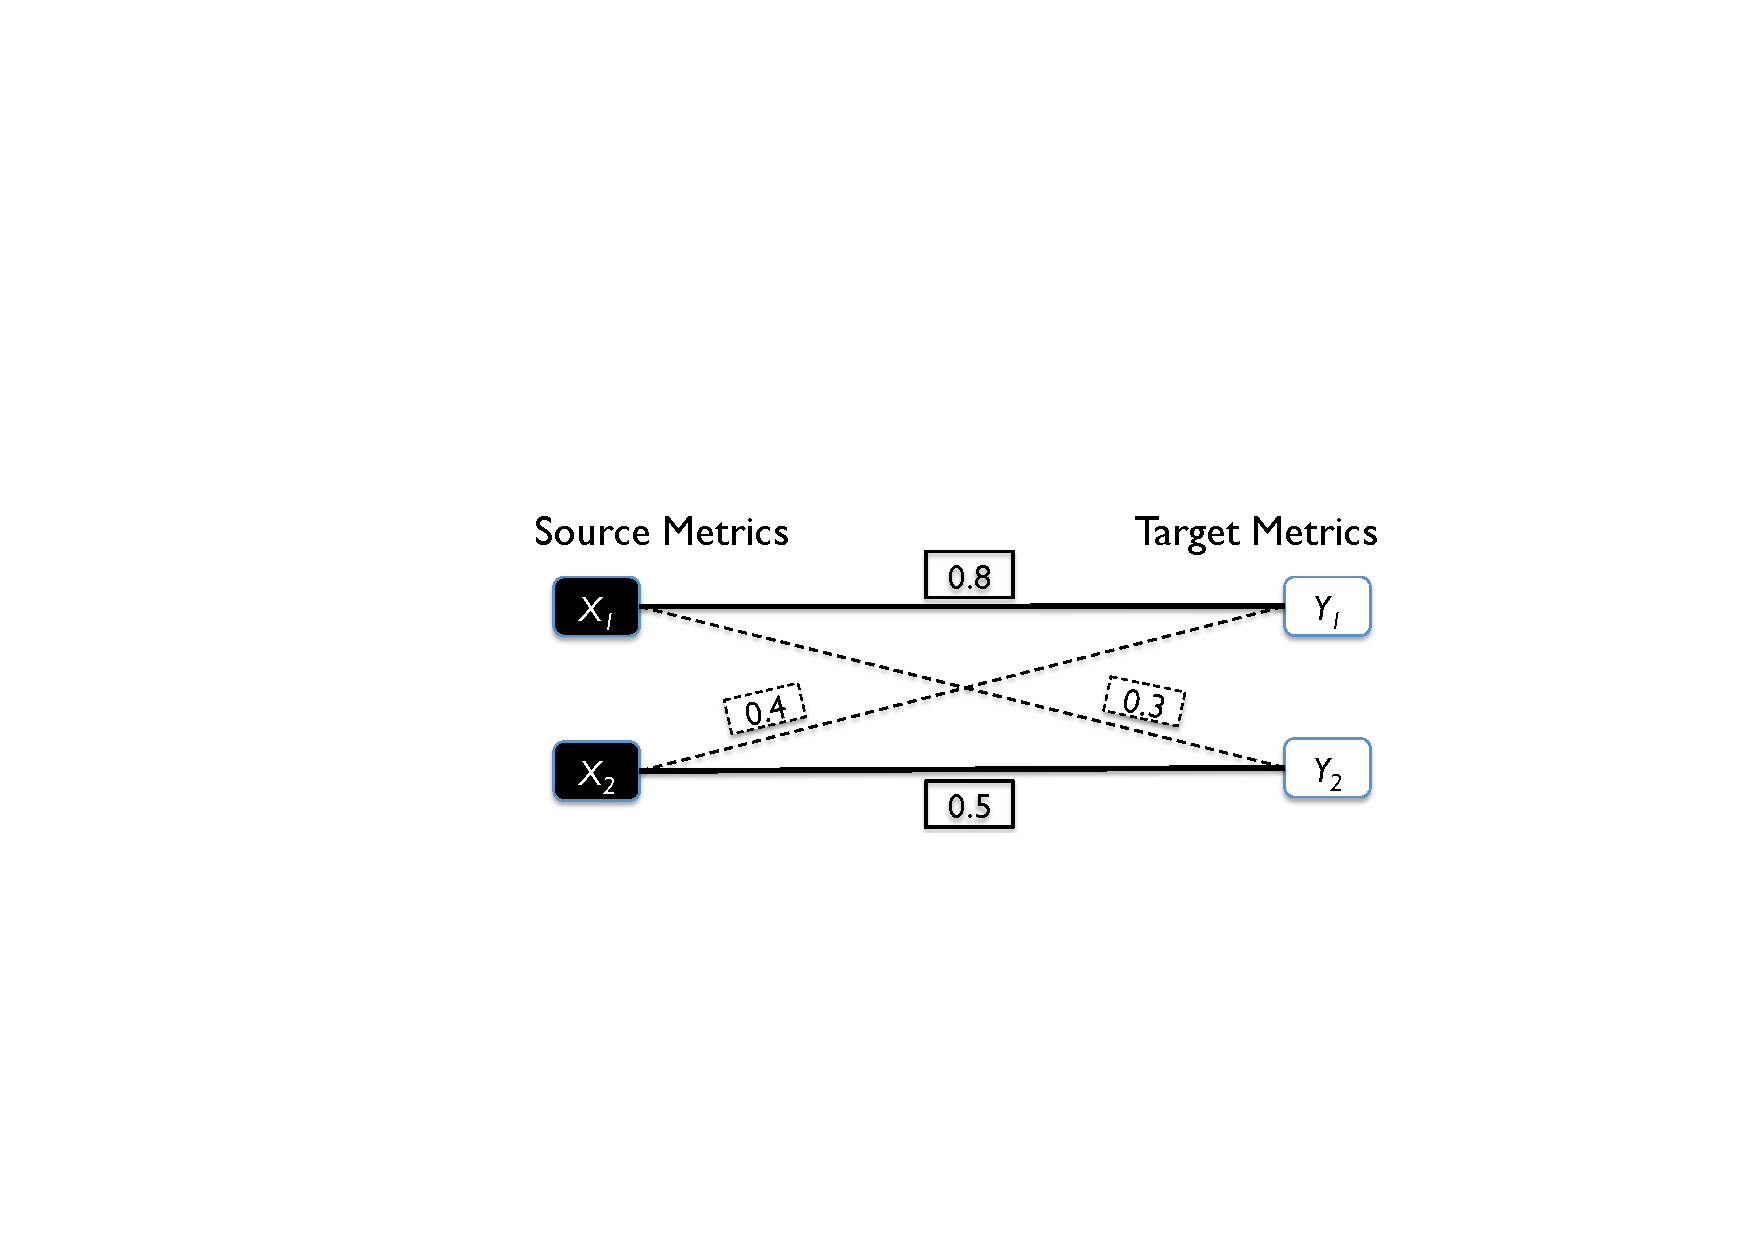
\includegraphics[width=\linewidth]{Figures/matching.pdf}
	\caption{An example of metric matching between source and target
	datasets.}
	\label{fig:matching}
\end{figure}

The key idea of these analyzers is computing matching
scores for all pairs between the source and target metrics.
Figure~\ref{fig:matching} shows a sample
matching. There are two source metrics ($X_1$ and $X_2$) and
two target metrics ($Y_1$ and $Y_2$). Thus, there are four possible matching
pairs, ($X_1$,$Y_1$), ($X_1$,$Y_2$), ($X_2$,$Y_1$), and ($X_2$,$Y_2$). The
numbers in rectangles between matched source and target metrics in
Figure~\ref{fig:matching} represent matching scores computed by an analyzer. For example,
the matching score between the metrics, $X_1$ and $Y_1$, is 0.8.

From all pairs between the source and target metrics, we remove poorly matched
metrics whose matching score is not greater than a specific cutoff threshold.
For example, if the matching score cutoff threshold is 0.3, we include only the
matched metrics whose matching score is greater than 0.3. In
Figure~\ref{fig:matching}, the edge ($X_1$,$Y_2$) in matched metrics will be
excluded when the cutoff threshold is 0.3. Thus, all the candidate matching
pairs we can consider include the edges ($X_1$,$Y_1$), ($X_2$,$Y_2$), and
($X_2$,$Y_1$) in this example.
In Section~\ref{sec:Evaluation}, we design our empirical study under different
matching score cutoff thresholds to investigate their impact on prediction.

We may not have any matched metrics based on the cutoff threshold. In this
case, we cannot conduct defect prediction. In
Figure~\ref{fig:matching}, if the cutoff threshold is 0.9, none of the matched
metrics are considered for HDP so we cannot build a prediction model for the target
dataset. For this reason, we investigate target prediction coverage (i.e.,
what percentage of target datasets could be predicted?) in
our experiments.

After applying the cutoff threshold, we
used {\em the maximum weighted bipartite matching}~\cite{Matouek06} technique to
select a group of matched metrics, whose sum of matching scores is highest,
without duplicated metrics.
%We can form groups of matched features without redundant features.
In Figure~\ref{fig:matching}, after applying the cutoff threshold of 0.30, we
can form two groups of matched metrics without duplicated metrics. The first
group consists of the edges, ($X_1$,$Y_1$) and ($X_2$,$Y_2$), and another group
consists of the edge ($X_2$,$Y_1$). In each group, there are no duplicated
metrics. The sum of matching scores in the first group is 1.3 (=0.8+0.5) and that of the second
group is 0.4.
The first group has a greater sum (1.3) of matching scores than the
second one (0.4). Thus, we select the first matching group as the set of
matched metrics for the given source and target metrics with the cutoff
threshold of 0.30 in this example.
%that can be solved
% by a linear program in polynomial time~\cite{Matouek06}.
 
% Based on the co-occurrence features, we can
% generate new source and target datasets with only the co-occurrence features.
% For example, as shown in Figure~\ref{fig:framework}, the datasets of Project A
% and B have three (after feature selection) and eight features respectively and
% two sets of features (dashed lines) are identified as co-occurrence features. With
% these co-occurrence features, we can generate new source and target datasets
% with a two-feature set as in Figure~\ref{fig:framework}. We designed various
% co-occurrence analyzers, which are explained in Section~\ref{sec:analyzers}.
% 


% as
% explained in Section~\ref{sec:Background}. Among them, we use
% ASAnalyzer with Filters investigated in Section~\ref{sec:ASAnalyzer}. 

% The cross-prediction runner conducts actual cross-domain defect prediction. The
% runner builds a prediction model by using a new source dataset and predicts
% the defects on a new target dataset. To our knowledge, cross-domain defect
% prediction is the first study on defect prediction using datasets with different
% feature spaces.


% \subsection{Feature Matching Analyzers} %Identifying co-occurrence features}
% \label{sec:analyzers}
% To identify co-occurrence features between source and target datasets, we
% design five co-occurrence feature analyzers as follows:
% \squishlist
% 	\item Average and Standard deviation analyzer (ASAnalyzer)
% 	\item T-test analyzer (TAnalyzer) 
% 	\item Pearson's correlation analyzer
% (PCoAnalyzer)
% 	\item Spearman's correlation analyzer (SCoAnalyzer) 
% 	\item Popularity index analyzer (PiAnalyzer) 
% \squishend

% Before applying analyzers, all feature values
% of datasets are normalized between 0 and 1 to avoid no individual feature has
% greater influence than others~\cite{Kocaguneli13}.

Each analyzer for the metric matching scores is described in the following subsections.

\subsubsection{PAnalyzer}
PAnalyzer simply compares 9 percentiles (10th, 20th,\ldots, 90th) of ordered
values between source and target metrics.

First, we compute the difference of $n$-th
percentiles in source and target metric values by the following
equation:
\begin{equation}
P_{ij}(n)=\frac{sp_{ij}(n)}{bp_{ij}(n)}
\end{equation}
, where $P_{ij}(n)$ is the comparison function for $n$-th percentiles
of $i$-th source and $j$-th target metrics, and $sp_{ij}(n)$ and $bp_{ij}(n)$
are smaller and bigger percentile values respectively at $n$-th percentiles
of $i$-th source and $j$-th target metrics. For example, if the 10th
percentile of the source metric values is 20 and that of target metric values is
15, the difference is 0.75 ($P_{ij}(10)=15/20=0.75$).

Using this percentile comparison function, a matching score between source
and target metrics is calculated by the following equation:
\begin{equation}
M_{ij}=\frac{\sum\limits_{k=1}^9
P_{ij}(10\times{k})}{9}\end{equation}
, where $M_{ij}$ is a matching score between $i$-th source and $j$-th
target metrics. The best matching score of this equation is 1.0
when the values of the source and target metrics of all 9 percentiles are the
same.

\subsubsection{KSAnalyzer}
KSAnalyzer uses a p-value from the Kolmogorov-Smirnov Test (KS-test)
as a matching score between source and target metrics. The KS-test is a
non-parametric two sample test that can be applicable when we cannot be sure
about the normality of two samples and/or the same
variance~\cite{Lilliefors67,Massey51}. Since metrics in some defect datasets
used in our empirical study have exponential distributions~\cite{Menzies07} and
metrics in other datasets have unknown distributions and variances, the KS-test
is a suitable statistical test to compute p-values for these datasets. In statistical testing, a p-value shows the
probability of whether two samples are significantly different or not. We used
the {\em KolmogorovSmirnovTest} implemented in the {\em Apache commons math}
library.


The matching score is:
\begin{equation}M_{ij}=p_{ij}\end{equation}
, where $p_{ij}$ is a p-value from the KS-test of $i$-th source and $j$-th
target metrics. A p-value tends to be zero when two metrics are significantly
different.

\subsubsection{SCoAnalyzer}
In SCoAnalyzer, we used the Spearman's
rank correlation coefficient as a matching score for source and target
metrics~\cite{Spearman10}.
Spearman's rank correlation measures how two samples
are correlated~\cite{Spearman10}. To compute the coefficient, we used the
{\em SpearmansCorrelation} in the {\em Apache commons math} library. Since the
size of metric vectors should be the same to compute the coefficient, we
randomly select metric values from a metric vector that is of a greater size
than another metric vector. For example, if the sizes of the source and target metric
vectors are 110 and 100 respectively, we randomly select 100 metric values from the
source metric to agree to the size between the source and target metrics. All
metric values are sorted before computing the coefficient.

The matching score is as follows:
\begin{equation}M_{ij}=c_{ij}\end{equation}
, where $c_{ij}$ is a Spearman's rank correlation coefficient between $i$-th
source and $j$-th target metrics.

% \subsubsection{Popularity Index (PiAnalyzer)}
% We adopted the
% concept of popularity index to identify similar source and target
% metrics~\cite{Kocaguneli13}.
% The popularity index was proposed by Kocaguneli et al. to discard redundant
% metrics and outlier instances for effort estimation~\cite{Kocaguneli13}.
% Popularity index represents how many times a metric or an instance is a nearest
% neighbor of other metrics or instances~\cite{Kocaguneli13}.
% 
% To match source and target
% metrics based on the popularity index, we proceed with the following steps:
% \squishlist
%   \item{Step 1:} Select and sort source and target instances by popularity
%   index.\footnote{Please, refer to the study of Kocaguneli et al.
% for details of the popularity index~\cite{Kocaguneli13}.}
%   This selection process makes the number of instances same in both source and
%   target datasets.
%   \item {Step 2:} Compute a matching score for each pair of source and target
%   metrics in the datasets consisting of instances from Step 1. The matching
%   score is:
% 		\begin{equation}M_{ij}=1-norm(E_{ij})\end{equation}
% 	, where $E_{ij}$ is a Euclidean distance between $i$-th source and $j$-th
% 	target metrics and $norm(x)$ is the normalization function to make $x$ range
% 	from zero to one. The matching score tends to be one when the distance between $i$-th source and $j$-th
% 	target metrics, $E_{ij}$, is closest.
% 	\item {Step 3:} Find a nearest neighbor of each source metric by using
% 	sorted matching scores from Step 2.
% \squishend
% After executing Step 3, we can match metrics between the
% source and target based on the popularity index.

% \begin{table}[t]
% \small
% \centering
% \caption{Comparison of Co-occurrence analyzers in terms of average AUC for
% 600 cross predictions from 28 defect datasets. (The matching score cutoff is
% 0.00. This means we use all matched features for training and test models.)}
% \label{tab:DiffAnalyzers}
% %\setlength{\tabcolsep}{5pt}
% %\setlength{\extrarowheight}{1.5pt}
% \begin{tabular}{|c|c|}
% \hline
% Analyzer	& Average AUC	\\\hline \hline
% ASAnalyzer	& 0.58	\\\hline
% TAnalyzer	& 0.58	\\\hline
% PCoAnalyzer	& 0.52	\\\hline
% SCoAnalyzer	& 0.51	\\\hline
% PiAnalyzer	& 0.57	\\\hline
% \end{tabular}
% \end{table}

\subsection{Building Prediction Models}

After applying metric selection and matching, we can finally build a
prediction model using a source dataset with selected and matched metrics. Then,
as a regular defect prediction model, we can predict defects on a target dataset
with the matched metrics.

\section{Experimental Setup}
\label{sec:Evaluation}
This section presents the details of our experimental study such as benchmark datasets, experimental design, and evaluation measures.
%In RQ1, we validate
% prediction models built by defect datasets. In addition, we were interested
% in verifying if our framework can build prediction models from non-defect
% datasets. Thus, in RQ2, we check prediction performance of models built by
% different types of non-defect datasets: software engineering (SE) and non-SE datasets.
% We conducted experiments using 28 defect datasets in 5 groups with different
% metric sets.


% The RQ3 is to verify whether our cross-domain prediction models can conduct
% cross-prediction for all target projects. Prediction coverage~\sung{Should we mention this in the approach? If we don't have any matching features based on your threshold, we cannot predict? Then, say, we investigate this in experiments.} represents how
% many target projects could be predicted by using our cross-domain models. If
% there are no feasible~\sung{Need to explain in detail in Approach.} prediction combinations for a certain target project, it
% might be difficult to use a cross-domain prediction model in practice.
%In previous studies on cross-project defect prediction,
%feasibility rate of cross prediction combinations were quite low (about
%3-5\%)~\cite{He12,Zimmermann09}.
% Thus, we address RQ3 by measuring prediction coverage.
\subsection{Benchmark Datasets}

\begin{table}[t]
%\scriptsize
\centering
\caption{The 34 defect datasets from five groups.}
\label{tab:datasets}
%\setlength{\tabcolsep}{5pt}
%\setlength{\extrarowheight}{1.5pt}
\begin{tabular}{|@{}c@{}|@{}c@{}|c|c|@{}c@{}|@{}c@{}|}
\hline
	\multirow{2}{*}{\textbf{Group}}
	&\multirow{2}{*}{\textbf{Dataset}}
	&\multicolumn{2}{c|}{\textbf{\# of instances}}
	&\multirow{2}{*}{\textbf{\specialcell{\# of\\metrics}}}
	&\multirow{2}{*}{\textbf{\specialcell{Prediction \\ Granularity}}}
	\\ \cline{3-4}
	
	&
	&\textbf{All}
	&\textbf{Buggy(\%)}
	&
	&
	\\ \hline \hline
\multirow{5}{*}{\specialcell{AEEEM~\\\cite{DAmbros12,Nam13}}}
	&	EQ
	&\centering324
	&	129 (39.81\%)
	& \multirow{5}{*}{61}
	& \multirow{5}{*}{Class}
	\\ %\cline{4-5}

	&	JDT
	&\centering997
	& 206 (20.66\%)
	& &
	\\ 

	&	LC	
	&\centering691
	& 64 (9.26\%)
	& &
	\\ 
	
	&	ML	
	&\centering1862
	& 245 (13.16\%)
	& &
	\\ 
	
	&	PDE
	&\centering1492
	& 209 (14.01\%)
	& &
	\\ \hline
	
\multirow{3}{*}{\specialcell{ReLink\\\cite{Wu11}}}
	&	Apache
	&\centering194
	&	98 (50.52\%)
	& \multirow{3}{*}{26}
	& \multirow{3}{*}{File}
	\\ %\cline{4-5}

	&	Safe
	&\centering56
	& 22 (39.29\%)
	& &
	\\ 
	
	&	ZXing
	&\centering399
	& 118 (29.57\%)
	& &
	\\ \hline
% \multirow{3}{*}{MIM~\cite{Lee11}}
% 	&	MIMEtc
% 	&\centering1042
% 	&	57(5.40\%)
% 	& \multirow{3}{*}{113}
% 	\\ %\cline{4-5}
% 
% 	&	MIMMylyn
% 	&\centering1061
% 	& 152(14.30\%)
% 	& 
% 	\\ 
% 	
% 	&	MIMTeam
% 	&\centering239
% 	& 85(35.50\%)
% 	& 
% 	\\ \hline
	
\multirow{10}{*}{\specialcell{MORPH\\\cite{Peters12}}}
	&	ant-1.3
	&\centering125
	&	20 (16.00\%)
	& \multirow{10}{*}{20}
	& \multirow{10}{*}{Class}
	\\ %\cline{4-5}

	&	arc
	&\centering234
	& 27 (11.54\%)
	& &
	\\ 
	
	&	camel-1.0
	&\centering339
	& 13 (3.83\%)
	& &
	\\
	
	&	poi-1.5
	&\centering237
	& 141 (59.49\%)
	& &
	\\ 
	
	&	redaktor
	&\centering176
	& 27 (15.34\%)
	& &
	\\ 
	
	&	skarbonka
	&\centering45
	& 9 (20.00\%)
	& & 
	\\ 
	
	&	tomcat
	&\centering858
	& 77 (8.97\%)
	& &
	\\ 
	
	&	velocity-1.4
	&\centering196
	& 147 (75.00\%)
	& &
	\\ 
	
	&	xalan-2.4
	&\centering723
	& 110 (15.21\%)
	& &
	\\ 
	
	&	xerces-1.2
	&\centering440
	& 71 (16.14\%)
	& &
	\\ \hline

\multirow{11}{*}{\specialcell{NASA\\\cite{promise12,Shepperd13}}}
	&	cm1
	&\centering344
	&	42 (12.21\%)
	& \multirow{5}{*}{37}
	& \multirow{11}{*}{Function}
	\\ %\cline{4-5}

	&	mw1
	&\centering264
	& 27 (10.23\%)
	& &
	\\

	&	pc1
	&\centering759
	& 61 (8.04\%)
	& &
	\\

	&	pc3
	&\centering1125
	& 140 (12.44\%)
	& &
	\\

	&	pc4
	&\centering1399
	& 178 (12.72\%)
	& &
	\\ \cline{2-5}

	&	jm1
	&\centering9593
	& 1759 (18.34\%)
	& 21 &
	\\ \cline{2-5}

	&	pc2
	&\centering1585
	& 16 (1.01\%)
	& 36 &
	\\ \cline{2-5}

	&	pc5
	&\centering17001
	& 503 (2.96\%)
	& 38 &
	\\ 

	&	mc1
	&\centering9277
	& 68 (0.73\%)
	& 38 &
	\\ \cline{2-5}

	&	mc2
	&\centering127
	& 44 (34.65\%)
	& 39 &
	\\

	&	kc3
	&\centering200
	& 36 (18.00\%)
	& 39 &
	\\ \hline
	
\multirow{5}{*}{\specialcell{SOFTLAB\\\cite{Turhan09}}}
	&	ar1
	&\centering121
	&	9 (7.44\%)
	& \multirow{5}{*}{29}
	& \multirow{5}{*}{\specialcell{Function}}
	\\ %\cline{4-5}

	&	ar3
	&\centering63
	& 8 (12.70\%)
	& &
	\\ 

	&	ar4
	&\centering107
	& 20 (18.69\%)
	& &
	\\ 
	
	&	ar5	
	&\centering36
	& 8 (22.22\%)
	& &
	\\ 
	
	&	ar6
	&\centering101
	& 15 (14.85\%)
	& &
	\\ \hline	

\end{tabular}
\end{table}

We collected publicly available datasets from previous
studies~\cite{DAmbros12,Nam13,Peters12,Turhan09,Wu11}.
Table~\ref{tab:datasets} lists all dataset groups used in our experiments. Each
dataset group has a heterogeneous metric set as shown in the table.
Prediction Granularity in the last column of the table means the prediction
granularity of instances. Since we focus on the distribution or correlation of
metric values when matching metrics, it is beneficial to be able to
apply the HDP approach on datasets even in different granularity levels.
% Table~\ref{tab:SE_datasets} and~\ref{tab:non-SE_datasets} list
% non-defect (SE and non-SE) datasets, which were used only for training
% prediction models in our study.

% \begin{figure}[t]
% 	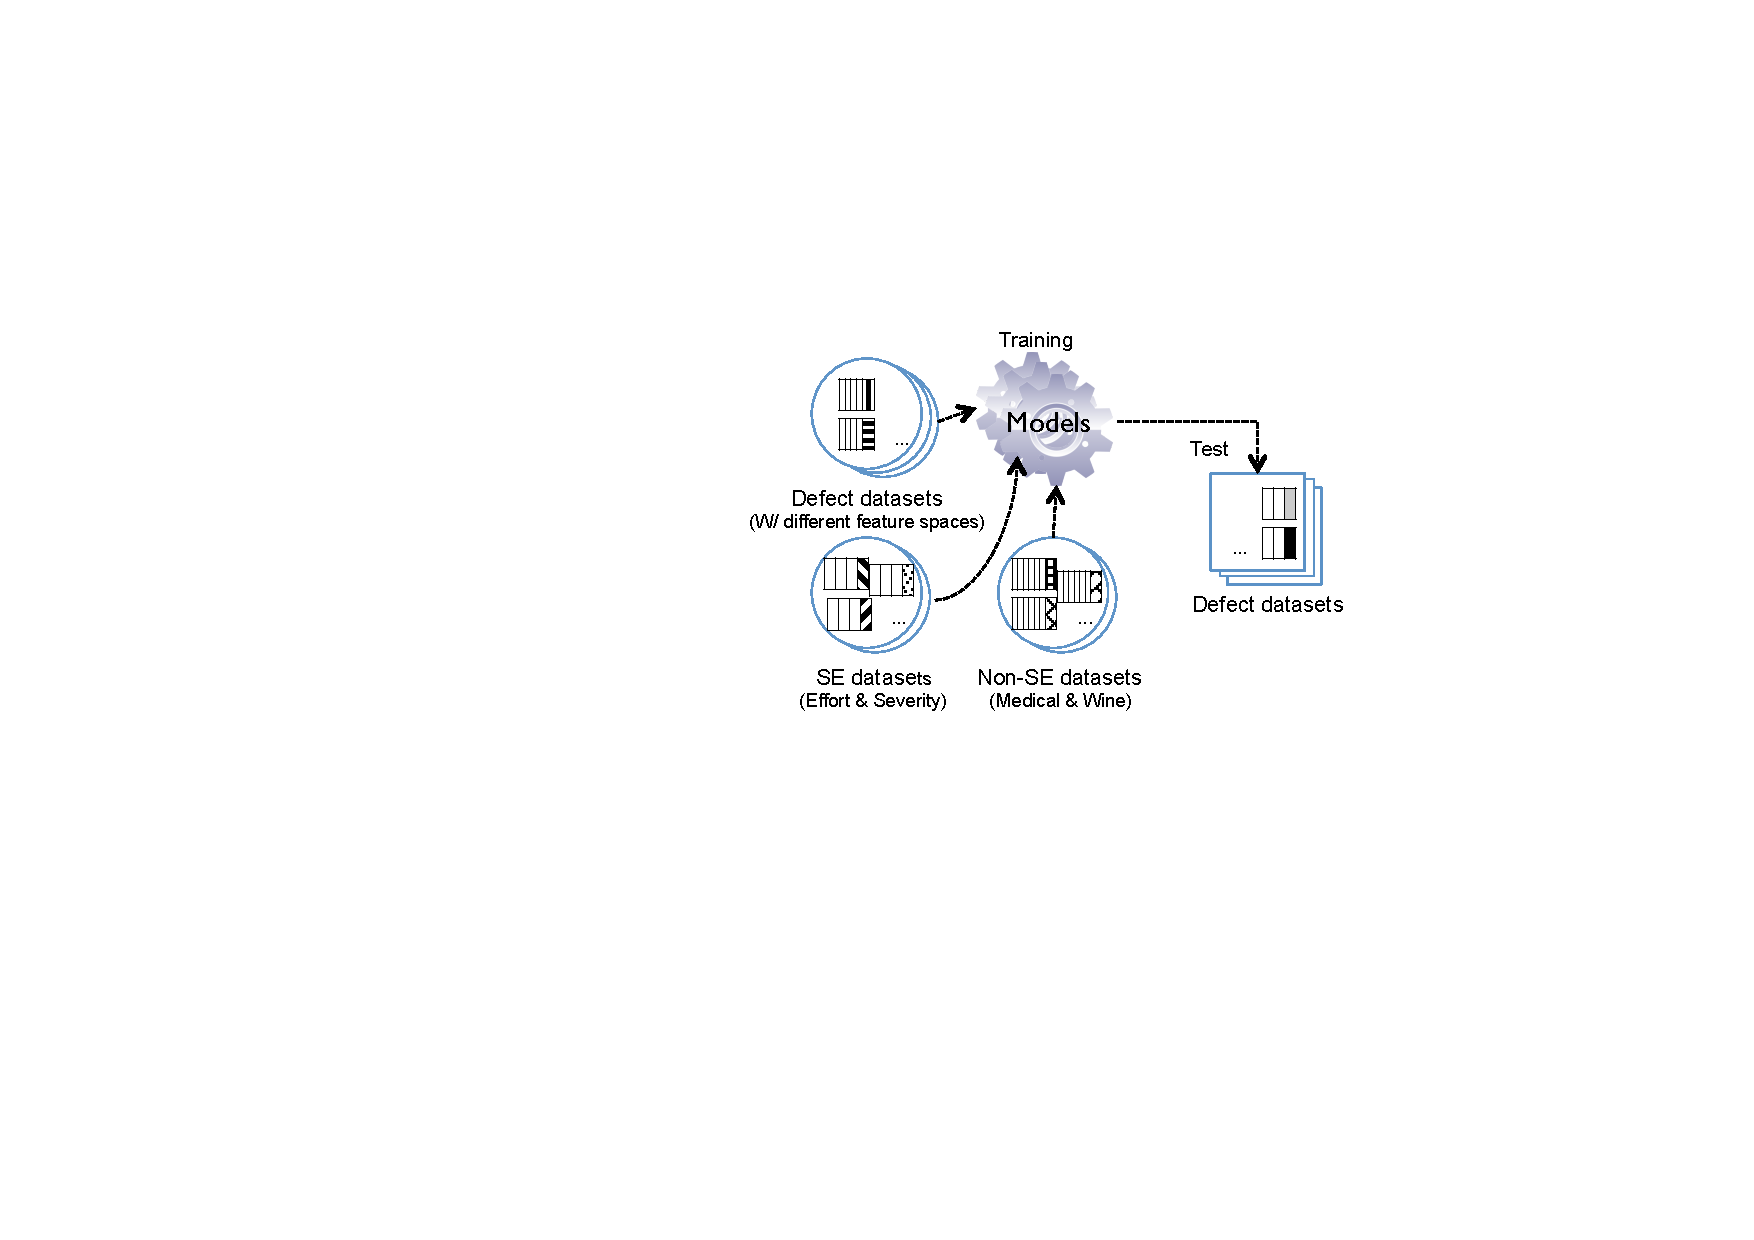
\includegraphics[width=\linewidth]{Figures/overview.pdf}
% 	\caption{Overview of cross-domain defect prediction across benchmark datasets.}
% 	\label{fig:overview}
% \end{figure}
% 
% Figure~\ref{fig:overview} describes the overview of our cross-domain defect
% prediction across benchmark datasets. We validated our framework using
% models built by defect, SE, or non-SE for testing defect datasets.

We used five groups with 34 defect datasets: AEEEM, ReLink, MORPH, NASA,
and SOFTLAB.

AEEEM was used to benchmark different defect
prediction models~\cite{DAmbros12} and to evaluate CPDP
techniques~\cite{He14,Nam13}.
Each AEEEM dataset consists of 61 metrics including object-oriented (OO) metrics,
previous-defect metrics, entropy metrics of change and code, and churn-of-source-code
metrics~\cite{DAmbros12}.

Datasets in ReLink were used by Wu et
al.~\cite{Wu11} to improve the defect prediction performance by increasing the quality of the
defect data and have 26 code complexity metrics extracted by the Understand
tool~\cite{Understand}.

The MORPH group contains defect datasets of several open source projects used in
the study about the dataset privacy issue for defect prediction~\cite{Peters12}.
The 20 metrics used in MORPH are McCabe's cyclomatic metrics, CK metrics, and
other OO metrics~\cite{Peters12}.

NASA and SOFTLAB contain proprietary
datasets from NASA and a Turkish software company, respectively~\cite{Turhan09}.
We used 11 NASA datasets in the PROMISE
repository~\cite{promise12,Shepperd13}. Some NASA datasets have different metric sets as shown in Table~\ref{tab:datasets}. We used cleaned NASA datasets (DS$'$ version)~\cite{Shepperd13}.
For the SOFTLAB group, we used all SOFTLAB datasets in the PROMISE
repository~\cite{promise12}. The metrics used in both NASA and SOFTLAB groups
are Halstead and McCabe's cyclomatic metrics but NASA has additional
 complexity metrics such as {\em parameter count} and {\em percentage of comments}~\cite{promise12}.

Predicting defects is conducted across different dataset
groups.
For example, we build a prediction model by Apache in ReLink and tested the
model on velocity-1.4 in MORPH
(Apache$\Rightarrow$velocity-1.4).\footnote{Hereafter a rightward arrow
($\Rightarrow$) denotes a prediction combination.} Since some NASA datasets do not have the same metric sets, we also conducted cross prediction between some NASA datasets that have different metric sets, e.g, (cm1$\Rightarrow$jm1).

We did not conduct defect prediction across projects where datasets have the same metric set since the focus of our study is on prediction
across datasets with heterogeneous metric sets.
% We represent this prediction combination as EQ$\Rightarrow$Apache. We use the same representation,
% SOURCE$\Rightarrow$Target, for other prediction combinations across the paper.
In total, we have 962 possible prediction combinations from these 34 datasets. Since we select top 15\% of metrics for metric selection as explained in Section~\ref{sec:metricselection}, the number of selected metrics varies from 3 (MORPH) to 9 (AEEEM)~\cite{Gao11}.

% \begin{table}[t]
% \small
% \centering
% \caption{Non-defect  SE datasets to build prediction models. Task column stands for
% original tasks of datasets. Tasks can be multiclass classification (M) or regression (R).}
% \label{tab:SE_datasets}
% %\setlength{\tabcolsep}{5pt}
% %\setlength{\extrarowheight}{1.5pt}
% \begin{tabular}{|@{ }c@{ }|@{ }c@{ }|@{ }c@{ }|@{ }c@{ }|@{ }c@{ }|@{
% }c@{ }|}
% \hline
% 	\multirow{2}{*}{\textbf{Type}}
% 	&\multirow{2}{*}{\textbf{Dataset}}
% 	&\multicolumn{2}{c|}{\textbf{\# of instances}}
% 	&\multirow{2}{*}{\textbf{\specialcell{\# of\\features}}}
% 	&\multirow{2}{*}{\textbf{Task}}
% 	\\ \cline{3-4}
% 	&
% 	& All
% 	& Buggy(\%)
% 	&
% 	&
% 	\\ \hline \hline
% Effort
% 	&	albrecht
% 	&\centering24
% 	&	12(50.00\%)
% 	& 7
% 	& R
% 	\\ \hline
% 	
% Severity
% 	&	pitsB
% 	&\centering987
% 	& 964(97.67\%)
% 	& 1682
% 	& M
% 	\\ \hline
% % Medical
% % 	& Cancer	
% % 	&\centering253
% % 	& 162(64.03\%)
% % 	& 15154
% % 	& B 
% % 	\\ 	\hline
% % Wine
% % 	& Quality
% % 	&\centering4898
% % 	& 1640(33.48\%)
% % 	& 11
% % 	& M
% % 	\\ \hline
% \end{tabular}
% \end{table}
% 
% For SE datasets, we used two datasets, Effort~\cite{Kocaguneli13}
% and Severity~\cite{Menzies08}, as shown in Table~\ref{tab:SE_datasets}.
% We chose one representative dataset, which has the most number of instances in
% each referenced paper. These datasets are used only for training a model.
% Effort and Severity datasets were collected for software engineering studies,
% effort estimation~\cite{Kocaguneli13} and severity assessment of software defect
% reports~\cite{Menzies08}, respectively.
% 
% \begin{table}[t]
% \small
% \centering
% \caption{Non-SE datasets to build prediction models. Task column stands for
% original tasks of datasets. Tasks can be binary classification (B) or multiclass classification (M).}
% \label{tab:non-SE_datasets}
% %\setlength{\tabcolsep}{5pt}
% %\setlength{\extrarowheight}{1.5pt}
% \begin{tabular}{|@{ }c@{ }|@{ }c@{ }|@{ }c@{ }|@{ }c@{ }|@{ }c@{ }|@{ }c@{ }|@{
% }c@{ }|}
% \hline
% 	\multirow{2}{*}{\textbf{Type}}
% 	&\multirow{2}{*}{\textbf{Dataset}}
% 	&\multicolumn{2}{c|}{\textbf{\# of instances}}
% 	&\multirow{2}{*}{\textbf{\specialcell{\# of\\features}}}
% 	&\multirow{2}{*}{\textbf{Task}}
% 	\\ \cline{3-4}
% 	&
% 	& All
% 	& Buggy(\%)
% 	&
% 	&
% 	\\ \hline \hline
% 
% Medical
% 	& Cancer
% 	&\centering569
% 	& 212(37.26\%)
% 	& 30
% 	& B
% 	\\ 	\hline
% Wine
% 	& Quality
% 	&\centering4898
% 	& 1640(33.48\%)
% 	& 11
% 	& M
% 	\\ \hline
% \end{tabular}
% \end{table}
% 
% We used Medical~\cite{Street93}, and
% Wine~\cite{Cortez09} datasets for non-SE datasets.
% Medical and Wine datasets are from totally different areas.
% %The Medical dataset has inherently different characteristics but
% However, the prediction task of Medical dataset, predicting a medical `defect'
% (breast cancer), is similar to that of software defect prediction.
% Wine dataset was to predict the quality of wines. Using these datasets from
% different research areas would be interesting to evaluate our approach as well.
% 
% We build prediction models by each SE or non-SE dataset and test the models on
% all defect datasets. In total, we have 112 prediction combinations for
% SE and non-SE$\Rightarrow$defect.
% 
% We categorized non-defect datasets into three tasks:
% binary classification (B), multi-class classification (M), or regression (R).
% For a dataset of the B task, we can directly use class labels by matching them into buggy or clean to build
% prediction models. For example, two classes of the Medical dataset, Malignant
% and Benign, can be matched into buggy and clean, respectively.
% 
% Datasets of the M task have more than two class labels (nominal or ordinal
% values). Datasets of the R task have cardinal values. To build binary
% classification models for defect prediction in the M and R tasks, we should
% divide instances into two groups based on their values.
% The Effort dataset is labeled by the required development hours to finish a
% software project. As we assume fixing defects may require more development
% effort, we label Effort instances as clean when an instance has less than the
% median value of required development hours, otherwise as buggy.
% Severity dataset has five labels from NASA's severity scores (Severity 1 to 5).
% Issues with Severity 1 to 3 ``prevent or adversely affect the accomplishment of an essential
% capability''~\cite{Menzies08} while ones of Severity 4 and 5 do not. Thus, we
% labeled instances with Severity 1 to 3 as buggy and others as clean. The Wine
% dataset has the quality scores from 0 (low quality) to 10 (high quality). We
% marked Wine instances as clean when the quality score is more than 5, otherwise
% as buggy.

\subsection{Cutoff Thresholds for Matching Scores}

To build HDP models, we apply
various cutoff thresholds for matching scores to observe how prediction
performance varies according to different cutoff values. Matched metrics
by analyzers have their own matching scores as explained in
Section~\ref{sec:Approach}. We apply different cutoff values (0.05 and 0.10,
0.20,\ldots,0.90) for the HDP models. If a
matching score cutoff is 0.50, we remove matched metrics with the
matching score $\leq$ 0.50 and build a prediction model with matched metrics
with the score $>$ 0.50. The number of matched metrics varies by each prediction
combination. For example, when using KSAnalyzer with the cutoff of 0.05, the
number of matched metrics is four in cm1$\Rightarrow$ar5 while that is one in
ar6$\Rightarrow$pc3. The average number of matched metrics also varies by
analyzers and cutoff values; 4 (PAnalyzer), 2 (KSAnalyzer), and 5 (SCoAnalyzer)
in the cutoff of 0.05 but 1 (PAnalyzer), 1 (KSAnalyzer), and 4 (SCoAnalyzer) in
the cutoff of 0.90 on average.

\subsection{Baselines}

We compare HDP to three baselines: WPDP (Baseline1), CPDP using common
metrics (CPDP-CM) between source and target datasets (Baseline2), and CPDP-IFS
(Baseline3).

We first compare HDP to WPDP. Comparing HDP
to WPDP will provide empirical evidence of whether our
HDP models are applicable in practice.

% In addition, we compare cross-prediction results of our analyzers
% to those using common fetures. The random analyzer randomly matches source and
% target features. If cross-predictions by our analyzers can outperform those by
% the random analyzer, it implies that matching source and target features by
% co-occurrence analyzers is a meaningful way to realize cross-domain defect
% prediction.

We conduct CPDP using only common metrics (CPDP-CM) between
source and target datasets as in previous CPDP
studies~\cite{He14,Ma12,Turhan09}.
For example, AEEEM and MORPH have OO metrics as common metrics so we use them to build prediction
models for datasets between AEEEM and MORPH. Since
using common metrics has been adopted to address the limitation on heterogeneous
metric sets in previous CPDP studies~\cite{He14,Ma12,Turhan09}, we set CPDP-CM
as a baseline to evaluate our HDP models.
The number of common metrics varies across the dataset groups as ranged from 1 to 38. Between
AEEEM and ReLink, only one common metric exists, {\em LOC} (ck\_oo\_numberOfLinesOfCode : CountLineCode).
Some NASA datasets that have different metric sets, e.g., pc5 vs. mc2, have 38 common metrics. On average, the number of common
metrics in our datasets is about 12. We put all the common metrics between the five dataset groups in the online appendix: {\em https://lifove.github.io/hdp\#cm}.

We include CPDP-IFS proposed by He et al. as a
baseline~\cite{He14}. CPDP-IFS enables defect prediction on
projects with heterogeneous metric sets (Imbalanced Feature Sets) by using the
16 distribution characteristics of values of each instance such as mode, median,
mean, harmonic mean, minimum, maximum, range, variation ratio, first quartile,
third quartile, interquartile range, variance, standard
deviation, coefficient of variance, skewness, and kurtosis~\cite{He14}.
The 16 distribution characteristics are used as features to build a prediction model~\cite{He14}.
% Using common features for cross-predictions on datasets with different feature
% sets was used in previous cross-project/company defect prediction studies by Nam et al. and Turhan et al.~\cite{Nam13,Turhan09}.
% Comparing cross-results by manual feature matching using common features to
% those of our co-occurrence analyzers can provide guidelines for what makes good
% cross-predictions.



%In other words, matching scores computed by ScoAnalyzer and PiAnalyzer
%may not be helpful to judge how much matched features are similar or not.

%The average number of common features are five
% Since we apply feature selection for all source datasets before applying
% analyzers, other analyzers with the cutoff, 0.00, have the same number of
% matched features (2-6) on average. However, in the cutoff, 0.05, the average
% number of features is 1, 2, or 3.

% Random analyzer randomly identifies co-occurrence features for all possible
% matches so that the average number of matched features is about 20-26. In the
% case of manual feature matching, we found common features (4-10) across datasets
% and the matched features of each prediction combination are size, OO, Halstead,
% and/or cyclomatic metrics.



\subsection{Experimental Design}
\label{sec:expdesign}
%To evaluate our HDP models, we conducted
%extensive and large-scale experiments.
% We designed our experiments as follows:
% \squishlist
%   \item Evaluate our approach using ASAnalyzer with filters.
%   \item Repeat both within- and cross-predictions 1000 times for randomness of .
% \squishend

% We chose five machine learning algorithms widely used in defect prediction
% literature: J48 decision tree, Random forest, Naive Bayes, Bayesian network,
% Logistic regression, and Platt's SMO algorithm for Support Vector Machine (SVM).
% By the extensive experiments, we can confirm the best machine learning
% algorithm suggested from the previous defect prediction studies and get several
% insights to select a proper machine learning algorithm for cross-domain defect
% prediction as well. For the six algorithms, we used Weka
For the machine learning algorithm, we use seven widely used classifiers such as Simple logistic, Logistic regression, Random Forest, Bayesian Network, Support vector machine, J48 decision tree, and Logistic model tree~\cite{DAmbros12,Ghotra15,Lee11,Lessmann08,Nam13,Song11,Ghotra15}.
For these classifiers, we use Weka implementation with default
options~\cite{Weka}.

For WPDP, it is necessary to split datasets into training and test
sets. We use the two-fold cross validation (CV), which is widely used in the evaluation of
defect prediction models~\cite{Klas2010,Nam13,Pinzger2008}. In the two-fold CV, we use one half of the instances for training a model and the rest for
test (round 1). Then, we use the two splits (folds) in a reverse way, where we
use the previous test set for training and the previous training set for test
(round 2). We repeat these two rounds 500 times, i.e. 1000 tests, since there
is a randomness in selecting instances for each split~\cite{Arcuri11}. When conducting the two-fold CV, the stratified CV that keeps the buggy rate of the two folds same as that of the original datasets is applied as we used the default options in Weka~\cite{Weka}.

For CPDP-CM, CPDP-IFS, and HDP, we build a 
prediction model by using a source dataset and test the model on the same test
splits used in WPDP. Since there are 1000 different test
splits for a within-project prediction, the CPDP-CM, CPDP-IFS, and HDP models
are tested on 1000 different test splits as well.

These settings for comparing HDP to the baselines are for RQ1. The experimental settings for RQ2 is described in Section~\ref{sec:sizelimit} in detail.

% We use ASAnalyzer with Filters as a co-occurrence analyzer and 0.90 cutoff
% for our framework since this analyzer and cutoff leads to the best
% performance as shown in the preliminary results (Table~\ref{tab:DiffCutOffs}).
\subsection{Measures}
\label{sec:measure}
To evaluate the prediction performance, we use the area under the receiver
operating characteristic curve (AUC). Evaluation measures such as precision is highly affected by prediction thresholds and higher defective ratios (class imbalance) of datasets~\cite{Tantithamthavorn16}.
However, the AUC is known as a useful measure for comparing
different models and is widely used because AUC is unaffected by class imbalance
as well as being independent from the cutoff probability (prediction
threshold) that is used to decide whether an instance should be classified as
positive or negative~\cite{Giger12,Lessmann08,Rahman12,Song11,Tantithamthavorn16}.
Mende confirmed that it is difficult to compare the defect prediction
performance reported in the defect prediction literature since prediction
results come from the different cutoffs of prediction thresholds~\cite{Mende10}.
However, the receiver operating characteristic curve is drawn by both the true
positive rate (recall) and the false positive rate on  various prediction
threshold values.
The higher AUC represents better prediction performance and the AUC of 0.5 means
the performance of a random predictor~\cite{Rahman12}.

To measure the effect size of AUC results among baselines and HDP, we compute Cliff's $\delta$ that is a non-parametric effect size measure~\cite{romano06}. As Romano et al. suggested, we evaluate the magnitude of the effect size as follows: negligible ($|\delta|<$ 0.147), small ($|\delta|<$ 0.33), medium ($|\delta|<$ 0.474), and large (0.474 $\leq|\delta|$)~\cite{romano06}.

To compare HDP by our approach to baselines, we also use the
Win/Tie/Loss evaluation, which is used for performance comparison between
different experimental settings in many studies~\cite{Kocaguneli13,Li12,
Valentini03}. As we repeat the experiments 1000 times for a target project
dataset, we
conduct the Wilcoxon signed-rank test (p$<$0.05) for all AUC values in
baselines and HDP~\cite{Wilcoxon45}.
If an HDP model for the target dataset outperforms a corresponding
baseline result after the statistical test, we mark this HDP model as a `Win'.
In a similar way, we mark an HDP model as a `Loss' when the results of
a baseline are better than those of our HDP approach with statistical
significance.
If there is no difference between a baseline and HDP with statistical
significance, we mark this case as a `Tie'. Then, we count the number of
wins, ties, and losses for HDP models. By using the Win/Tie/Loss
evaluation, we can investigate how many HDP predictions it will take to improve
baseline approaches.




\begin{figure*}[t]
	\centering
% 	\vspace{0.5mm}
	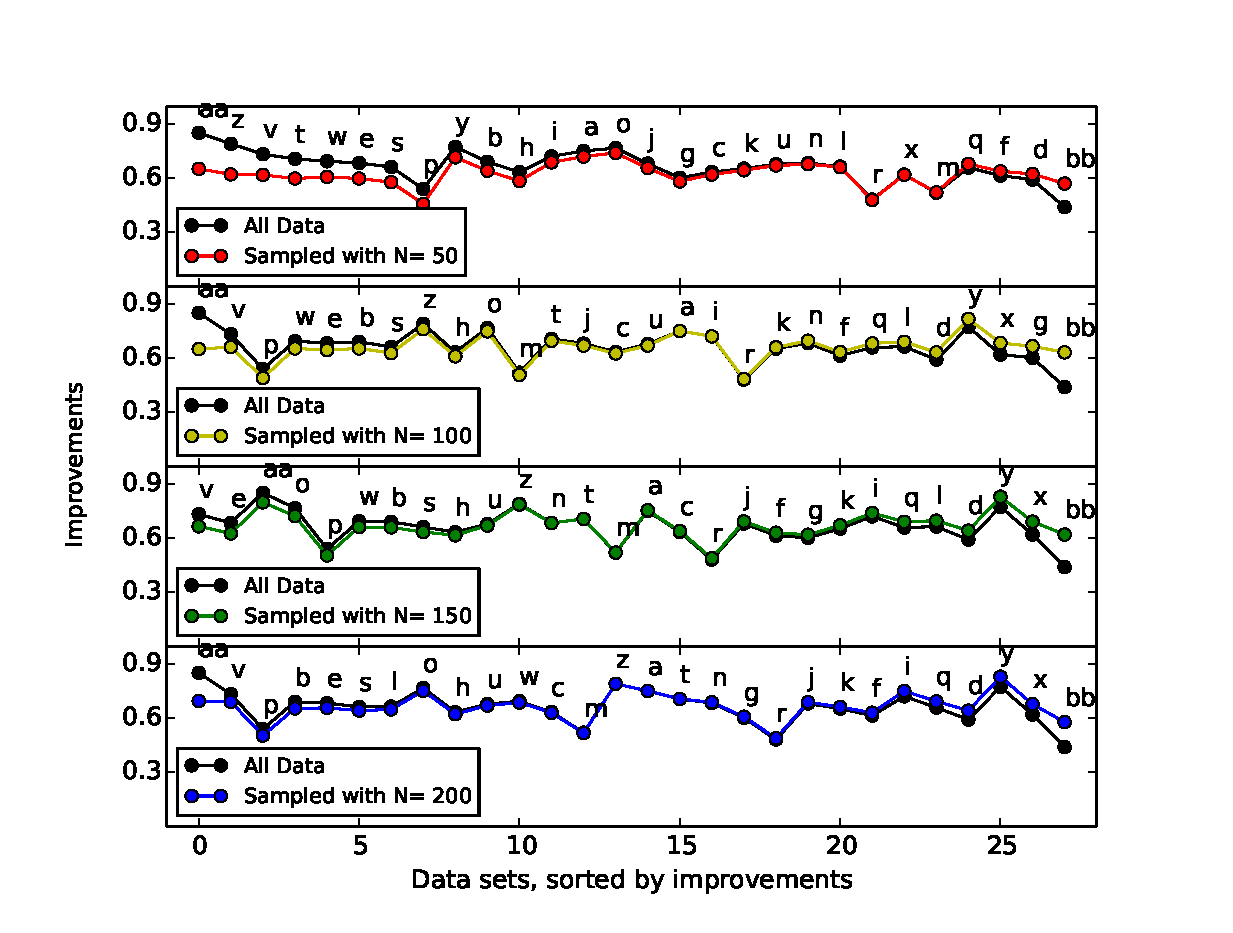
\includegraphics[width=.66\linewidth]{Figures/raleigh/sample_random.eps}
	\caption{Improvements of using sampled data over all data with sampled size N = \{50, 100, 150, 200\}. The Right side show  using small dataset is better than using all data. We label the data in table \ref{tab:datasets} from a to z, and continue from A to H, the last two datasets ar5 and ar6 as G and H.}
	\label{fig:small_data}
\end{figure*}

\section{Size Limits (lower bounds) for Effective Transfer Learning}
\label{sec:sizelimit}

In this section, we investigate the lower bounds of the effective sizes of source and target datasets for HDP models to address RQ2.

{\bf RQ2: What are the  lower  bounds  of  the  size  of source and target  datasets  for  effective HDP?}

Since HDP compares the distributions of source metrics to those of target metrics, it is important to seek the empirical evidence for the effective sizes of source and target datasets to match source and target metrics. We first present the results of the empirical study for RQ2 in this section and validate the generality of its results in Section~\ref{sect:xplain}.

Like prior work \cite{Nam13,
  Ma12, Rahman12, Ryu14,
  Zhang14}, the basic HDP method we
proposed above uses {\em all} the instances in potential source and target projects to perform metric to select the best matched metrics and then build
defect prediction learners.
Collecting {\em all} that data from source and target projects need much more work and also
for the target project, it requires waiting for it to finish before
transferring its learned lessons. This begs the question ``how early can we transfer?''.
That is, how {\em few} historical data and target projects do we need before transfer can be effective? In this section, we conduct an empirical study to answer these questions related to RQ2.

To investigate the size limits for effective transfer learning in the setting of CPDP across datasets with heterogeneous metric sets, we focus on the HDP approach. There are other approaches such as CPDP-IFS~\cite{He14} and CCA+~\cite{Jing15}. In Section~\ref{sec:Result}, we observed that HDP outperforms CPDP-IFS. In addition, CCA+ was evaluated in somewhat different context, i.e., cross-company defect prediction and with 14 projects which are far less than 34 projects used in our experiments for HDP. In addition, the implementation of CCA+ is not publicly available yet and more complex than HDP. For this reason, we conducted our empirical study for RQ2 based on HDP.




\subsection{Using Small Datasets is Feasible}

Recall from the above,
HDP uses  datasets  in a two step process.
To test the impact of having access to {\em less} data,
we  add an instance sampling process before performing metric matching:
instead of using all the instances from
candidate source and target datasets, those datasets will
be randomly sampled (without replacement) to generate smaller datasets of
size $N \in \{50, 100, 150, 200\}$.

The reason we choose those $N$ values as follows. On one hand, by looking at the size of datasets used in the
above experiment, we observed that minimum size is ar5 with $36$ instances and maximum size is pc5 with $17001$ instances.
The median and mean value of dataset size are $1505$ and $325$, respectively. Then $200$ is less than both of
them, which is reasonably small.
On the other hand, we use these numbers to show using small datasets is feasible compared to
the original. We're not claiming they're the best~(optimal) small numbers. For most datasets considered in this experiment, $N$ with these values is a
small data size compared to the original data size (e.g., we use $N \in \{50, 100, 150, 200\}$ whereas our datasets vary in size from 332 to 17001  median
to maximum number of rows).

When sampling the original data, {\it if
the number of instances in the original dataset is
smaller than $N$, all those instances will be
included}. For example, $N=200$ means we sampled both source and target data with size of $200$. If the dataset has less than $200$ instances, such as ar3, we use all
the instances and no oversampling is applied. With those sampled $N=200$ data, we perform metric matching to build a learner
and finally predict labels of all original data in the target project. We sample the data without replacement
to avoid duplicate data.

The results for this HDP-with-limited-data experiment is shown in \fig{small_data}
(we display median AUC results from 20 repeats, using  Logistic Regression
as the default learner).
% \lin{It's unclear to me. So metric matching on the 50, 100, etc.? What is third initial sampling? Add a backward reference to it? One caveat: I focused on reading the abstract, Section 3, 7, and 8, and I only skimmed over the rest of the paper, so maybe I missed it. But in general it is still good to add a backward reference.}\wei{I didn't get the question, "what is third initial sampling?", which third?}
% Since {\it Apahce commons math} library takes quite long time to conduct KS-test as mentioned, we replace it with Scipy, a python package, to speed up our experiment. \footnote{As shown in the table, the difference between those two KS-test results is acceptable}.
In that figure:
\squishlist
\item
  The {\em black} line show the results using {\em all} data;
\item
  The {\em colourful} lines show results of transferring from {\em some} small $N$ number of samples (instead of {\em all})
  in the source and target datasets during metric matching and learner building;
\item
  The letters show the unique ID of each dataset.
\squishend
% \begin{figure*}[t]
% 	\centering
% % 	\vspace{0.5mm}
% 	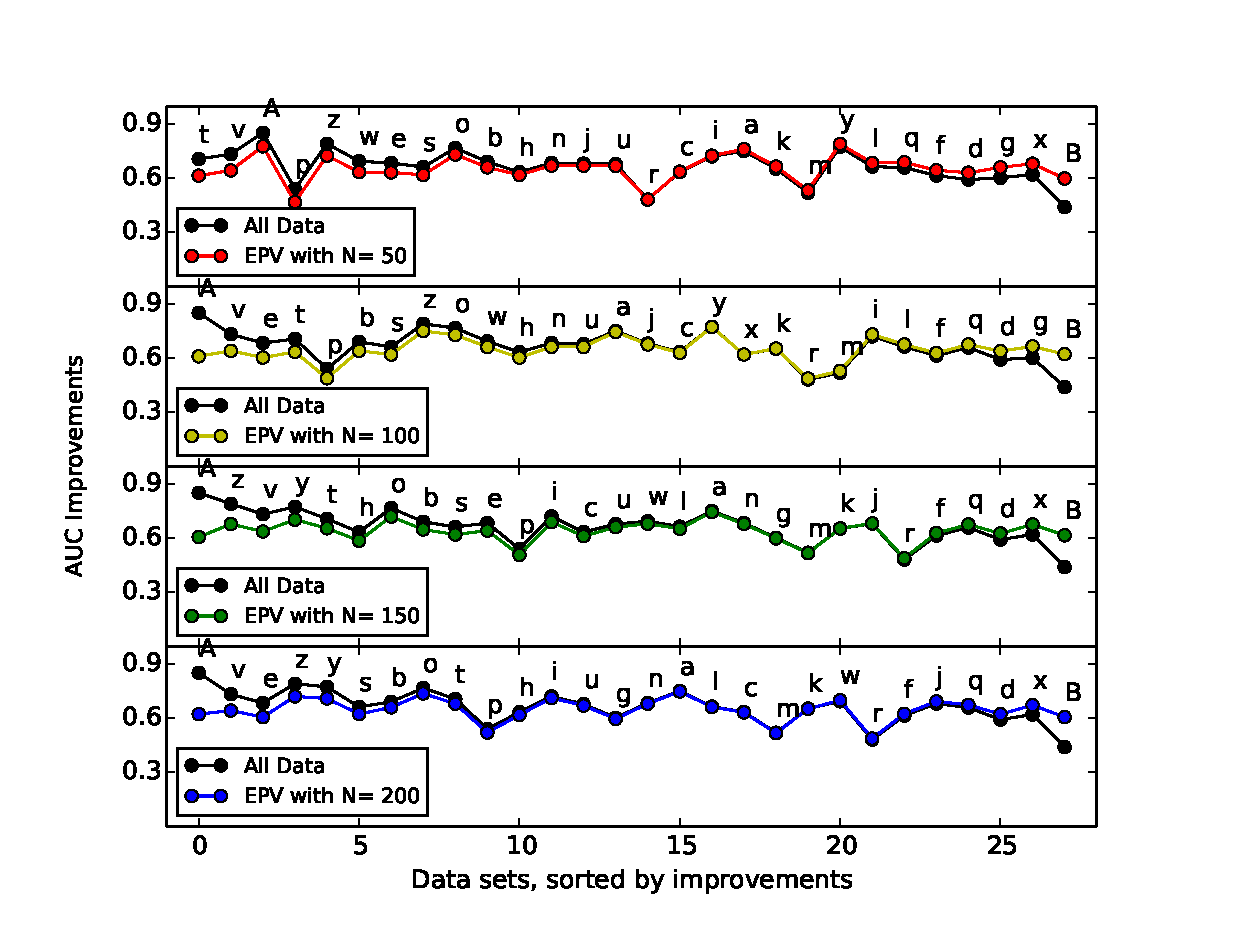
\includegraphics[width=0.66\linewidth]{Figures/raleigh/sample_epv.eps}
% 	\caption{Improvements of using sampled data N  = \{50, 100, 150, 200\} with EPV constraints. The Right side show  using small dataset with EPV is better than using all data. We label the data in table \ref{tab:datasets} from a to z, and continue from A to H, the last two datasets ar5 and ar6 as G and H.}
% 	\label{fig:small_epv}
% \end{figure*}
The datasets are ordered left to right by the difference to the black line (where we transfer using {\em
  all} the source data):
\squishlist
\item
  On the left, the black line is
  {\em above} the red line; i.e., for those datasets, we do {\em better} using
  {\em all} data than using {\em some}.
  \item
On the right, the black line is {\em below} the red
line; i.e., for those datasets, we do {\em worse}
using {\em all} data than using {\em some}.
\squishend
Note that the gap between the red and black line
shrinks as we use more data and after $N=100$, the
net gap space is almost zero.  When $N=200$, in $28/34$
datasets,
it is hard to distinguish
the blue and black curves of \fig{small_data}.
That is, we conclude
that using more
than a small sample size
(like $N=200$) would
not improve defect prediction.






% \subsection{20 Defective Examples  are Enough}


% The results of the last section are very encouraging---a small number of source
% and target examples are enough for effective transfer learning. Naturally,
% we were suspicious of this result (since it was ``almost too good to be true'').
% Accordingly, we explored the literature and found that:
% \squishlist
%     \item Evidence that this ``a few examples are enough'' has been seen in other domains~\cite{peduzzi1996simulation};
%     \item Further, we found new methods to reduce the cost of sampling this dataset, even further.
% \squishend
% Working in the domain cardiology,
%   Peduzzi et al.~\cite{peduzzi1996simulation}
%   report 10 ``events'' per variable (EPV) are enough to maximize the predictive performance
%   of  Logistic Regression (the learner used in this study). Translated into our terminology,
%   that study would predict that  10 defective data per independent variable should
%   suffice for effective learning. Of course, learners require defective and {\em non-defective}
%   examples so to $M$ defective examples, we add $(N-M)$ non-defective examples more.

%   To apply the method of Peduzzi et al., we first instrumented HDP to determine how many
%   independent variables were picked during {\em metric  selection}. In our previous experiments when using all source and target data to do feature/metric matching, we observed that the counts of matched features are as follows: $\{1:158, 2:78, 3:38, 4:9, 5:1\}$, where keys and values represent number of matched features, the corresponding counts of cross prediction combinations, respectively. Our read of this distribution is that the average number of matched features is about $2$. That means usually those 2 features from source and target projects can be used to build the learner. Hence, applying  Peduzzi et al.'s rule (EPV = $10$,  in our case, \# of events = $10$, \# of variables = $2$), we picked $2\times 10=20$ %\lin{why *10?}\wei{EPV=10, mentioned in the last paragraph. }
%   randomly selected defective data, then randomly added $(N-M)$ non-defective data for
%   $N\in \{50,100,150,200\}$ for the source data. For the target dataset, since we do not
%   know the data labels, we simply sampled $N$ for target data in metric matching.

%   (Aside: note that this is different to the above experiment since, before, the more $N$ examples
%   we selected, the more {\em defective} instances we would use. Now, in this experiment, we will also
%   use a fixed $M=20$ number of defective files and classes.).

%   The results are shown in \fig{small_epv}. Like before:
% \squishlist
%   \item These are median AUC results from 20 repeats;
% \item
%   The {\em black/colourful} lines show the results using {\em all/some} of  data from
%   the source and target datasets during metric matching and learner building, respectively
%   (but now, the {\em some} never contains more than $M=20$ defective instances);
% \item
%   The datasets are ordered left to right according
%   the performance difference between using
%   {\em all} or {\em some} of the data;
%   \item
%      On the left/right ,  we do {\em better/worse} using
%   {\em all} data than using {\em some}.
% \squishend
%   We observe that between $N=50$ and $N=200$, the performance delta
%   does not change by much. Also, if we compare $N=200$ between \fig{small_data}
%   and \fig{small_epv}, there is no large disadvantage of using just
%   $M=20$ defective instances.

%   Note that such a very small sample would be quick to collect: since training data is already available even before we start our target (new) project, we can easily sample $N$ data with $M=20$ defective classes/files for each candidate training data. After writing (say) a few
%   hundred classes for the target project, it's also easy to randomly sample $N$ from target project---at which point that data is a candidate for transfer learning.

\vspace{-0.5em}
\section{Result in AUC}
\label{sec:Result}
In this section, we report the experimental results of the HDP approach by
significance attribute selection for metric selection and KSAnalyzer with the cutoff threshold of 0.05.

Among different
metric selections, significance attribute selection led to the best
prediction performance overall. In terms of analyzers, KSAnalyzer led
to the best prediction performance.
Since the KSAnalyzer is based on the p-value of a statistical test, we chose
a cutoff of 0.05 which is a commonly accepted significance level in the
statistical test~\cite{Corder09}.

\vspace{-0.2em}
%----------------------------------------------------------
\subsection{Comparison Result with Baselines} % KSAnalyzer with the cutoff of %
% 0.05}
%----------------------------------------------------------

\begin{table}[!t]
%\footnotesize
%\small
\scriptsize
\centering
\caption{Comparison results among WPDP, CPDP-CM, CPDP-IFS,
and HDP by KSAnalyzer with the cutoff of 0.05 in a median AUC.
%  Outperforming results with statistical
%  significance (Wilcoxon signed-rank test, p$<$0.05) between within and cross by
%  the proposed approach and between cross using common features and those by the
%  proposed approach are bold-faced and underlined respectively.
}
\label{tab:result_overview}
%\setlength{\tabcolsep}{5pt}
%\setlength{\extrarowheight}{1.5pt}
\begin{tabular}{|@{ }c@{ }||@{ }c@{ }|@{ }c@{ }|@{ }c@{ }||@{ }c@{ }|}
%\begin{tabular}{|c||c|c|c||c|}
\hline
{\bf Target}
& \specialcell{{\bf WPDP}\\{(Baseline1)}} 
&\specialcell{{\bf CPDP-CM}\\{(Baseline2)}}
&\specialcell{{\bf CPDP-IFS}\\{(Baseline3)}}
&\specialcell{{\bf HDP}\\{\bf KSAnalyzer}\\{cutoff=0.05}}
\\
\hline \hline

EQ			&0.583	& 0.776	&0.461  &0.783		\\ \hline
JDT			&0.795	& 0.781 	&0.543	&0.767	 \\ \hline
LC			&0.575	& 0.636 &0.584	&0.655		\\ \hline
ML			&{\bf 0.734}	& 0.651 &0.557	&0.692*		\\ \hline
PDE			&0.684	& 0.682 &0.566	&0.717	 	\\ \hline \hline

Apache		&0.714	& 0.689  &0.635	&\underline{0.717}*		\\ \hline
Safe			&0.706	& 0.749  &0.616	&{\bf \underline{0.818}}*	 	\\ \hline
Zxing		&0.605	& 0.619  &0.530	&{\bf \underline{0.650}}*		\\ \hline \hline

ant-1.3		&0.609	& 0.590	&0.500	&0.835	 \\ \hline
arc			&0.670	& 0.611 &0.523	&0.701		\\ \hline
camel-1.0	&0.550	& 0.590	&0.500	&0.639	\\ \hline
poi-1.5		&0.707	& 0.676 &0.606	&0.701		\\ \hline
redaktor		&0.744	& 0.500 &0.500	&0.537		\\ \hline
skarbonka	&0.569	& 0.736 &0.528	&{\bf 0.694}*	 	\\ \hline
tomcat		&0.778	& 0.746 &0.640	&0.818		\\ \hline
velocity-1.4	& 0.725	& 0.609 &0.500	&0.391		\\ \hline
xalan-2.4	&0.755	& 0.658 &0.499	&0.751		\\ \hline
xerces-1.2	&0.624	& 0.453 &0.500	&0.489		\\ \hline \hline

cm1			&0.653	& 0.622 &0.551	&{\bf \underline{0.717}}*	 \\ \hline
mw1			&0.612	& 0.584 &0.614	& 0.727		\\ \hline
pc1			&0.787	& 0.675 &0.564	&0.752*		\\ \hline
pc3			&{\bf 0.794}	& 0.665 &0.500	&\underline{0.738}*		\\ \hline
pc4			&{\bf 0.900}	& 0.773 &0.589	&0.682*	 \\ \hline \hline

ar1		&0.582	& 0.464  &0.500	&{\bf \underline{0.734}}*		\\ \hline
ar3		&0.574	& 0.862 &0.682	&{\bf 0.823}*	 	\\ \hline
ar4		&0.657	& 0.588 &0.575	&{\bf \underline{0.816}}*	 \\ \hline
ar5		&0.804	& 0.875	&0.585	&0.911*	\\ \hline
ar6		&0.654	& 0.611 &0.527	&\underline{0.640}		\\ \hline \hline \hline

{\bf {\em All}} & 0.657 & 0.636 &0.555	& \underline{\bf 0.724}*  \\ \hline


\end{tabular}
\end{table}

% 
% \begin{figure*}[t]
% 	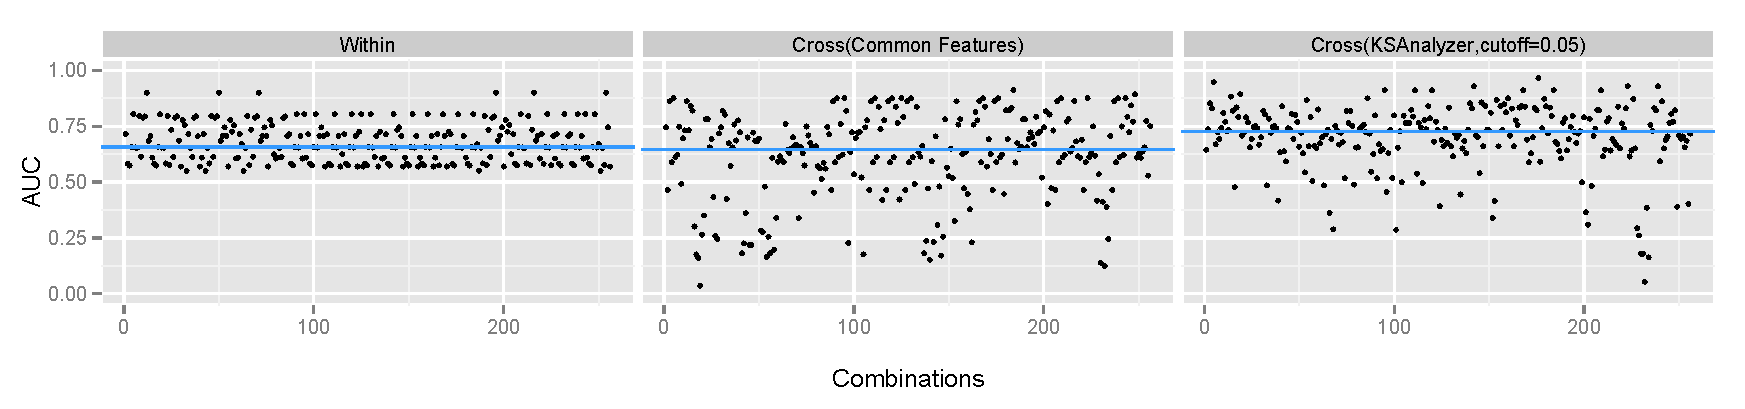
\includegraphics[width=\linewidth]{Figures/Result/auc_compare.pdf}
% 	\caption{Prediction performance variance among within-prediction,
% 	cross-prediction using common metrics, and cross-prediction by KSAnalyzer with
% 	the cutoff of 0.05 in terms of AUC. The number of prediction combinations is 256.}
% 	\label{fig:compare_results_on_defect}
% \end{figure*}


Table~\ref{tab:result_overview} shows the prediction performance (a median AUC)
of baselines and HDP by KSAnalyzer with the cutoff of 0.05,
for each target as well as all targets (the last row in the table). Baseline1 represents
the WPDP results of a target project and Baseline2 shows
the CPDP results using common metrics (CPDP-CM) between source and target
projects. Baseline3 shows the results of CPDP-IFS proposed by He et
al.~\cite{He14}. The last column shows the HDP results by KSAnalyzer with the
cutoff of 0.05. If there are better results between Baseline1 and our approach with statistical significance (Wilcoxon signed-rank
test~\cite{Wilcoxon45}, p$<$0.05), the better AUC values are in
bold font as shown in Table~\ref{tab:result_overview}.
Between Baseline2 and our approach, better AUC values with
statistical significance are underlined in
the table. Between Baseline3 and our approach, better AUC values with
statistical significance are shown with an asterisk (*).

%From Table~\ref{tab:result_overview}, 
We observed the following results about RQ1:
\squishlist
	\item In 25 out of 28 targets, HDP by KSAnalyzer with the cutoff of
	0.05 leads to better or comparable results against WPDP with statistical
	significance. (The WPDP results in only ML, pc3, and pc4 are in bold font.)
	\item HDP by KSAnalyzer with the cutoff of 0.05 outperforms
	WPDP with statistical significance when considering
	results from all targets ({\em All} in the last row in the table) together in
	our experimental settings.
\squishend  

The following results are related to RQ2:
\squishlist 	
	\item HDP by KSAnalyzer with the cutoff of 0.05
	leads to better or comparable results to CPDP-CM
	with statistical significance. (no underlines in CPDP-CM of
	Table~\ref{tab:result_overview})
	\item HDP by KSAnalyzer with the cutoff of 0.05 outperforms
	CPDP-CM with statistical significance
	when considering results from {\em All} targets in our experimental
	settings.
\squishend  

In terms of RQ3, we observed the following results:
\squishlist 	
	\item HDP by KSAnalyzer with the cutoff of 0.05
	leads to better or comparable results to CPDP-IFS with
	statistical significance. (no asterisks in CPDP-IFS of
	Table~\ref{tab:result_overview})
	\item HDP by KSAnalyzer with the cutoff of 0.05 outperforms
	CPDP-IFS with statistical significance
	when considering results from {\em All} targets in our experimental
	settings.
\squishend  
% Figure~\ref{fig:compare_results_on_defect} shows how the prediction performance
% of within- and cross-prediction varies. In
% Figure~\ref{fig:compare_results_on_defect}, each dot represents a prediction
% combination, e.g, EQ$\Rightarrow$Apache. In total, 222 dots (prediction
% combinations) are shown in each plot of the figure. The solid line in
% the figure represents the overall prediction performance, i.e. the median AUC
% values for prediction combinations.
% 
% Cross-results using common
% metrics show unstable results with large variance as in
% Figure~\ref{fig:compare_results_on_defect} where many prediction results are
% plotted under the AUC of 0.5.
% In addition, the median AUC (0.636) in cross-results using common metrics is
% slightly worse than that (0.657) in within-results. 
% 
% In cross-prediction by KSAnalyzer, some results are also plotted under the
% AUC of 0.5 because some cross-results by KSAnalyzer in the
% projects such as velocity-1.4 and xerces-1.2 have relatively low AUCs
% as shown in Table~\ref{tab:result_overview}.
% 
% However, note that the results by KSAnalyzer
% led to the best prediction performance in the median AUC and the variance of
% the results is smaller than cross-results using common metrics in
% Figure~\ref{fig:compare_results_on_defect}. The cross-result (0.724) of
% KSAanalyzer with the cutoff of 0.05 outperforms the within-result
% (0.657) and cross-result using common metrics (0.636) with statistical
% significance.

% We also compare
% cross-prediction results of AS, random analyzer, and manual matching as well. As we observe, the cross-result of AS outperforms that of both random analyzer and manual matching.

% \begin{table*}[t]
% \small
% \centering
% \caption{Within and cross-prediction results in median AUCs on various cutoff
% values. (W.=Within, C.=Cross) Better results between within- and
% cross-predictions are bold-faced (Mann-Whitney U-test, p$<$0.05).}
% \label{tab:DiffCutOffs}
% %\setlength{\tabcolsep}{5pt}
% %\setlength{\extrarowheight}{1.5pt}
% \begin{tabular}{|@{ }c@{ }||@{ }c@{ }|@{ }c@{ }|@{ }c@{ }||@{ }c@{
% }|@{ }c@{ }|@{ }c@{ }||@{ }c@{ }|@{ }c@{ }|@{ }c@{ }||@{ }c@{ }|@{ }c@{ }|@{
% }c@{ }|}
% \hline
% \multirow{2}{*}{{\bf Cutoffs}}	& \multicolumn{3}{c||}{{\bf PAnalyzer}} &
% \multicolumn{3}{c||}{{\bf KSAnalyzer}} &
% \multicolumn{3}{c||}{{\bf SCoAnalyzer}} &
% \multicolumn{3}{c|}{{\bf PiAnalyzer}} \\\cline{2-13}
% 	& {\bf W. AUC} & {\bf C. AUC} & {\bf \# comb.}
% 	& {\bf W. AUC} & {\bf C. AUC} & {\bf \# comb.}
% 	& {\bf W. AUC} & {\bf C. AUC} & {\bf \# comb.}
% 	& {\bf W. AUC} & {\bf C. AUC} & {\bf \# comb.} \\\hline
% \hline
% 0.00 & {\bf 0.683} & 0.641 & 600 & 0.664 & 0.686 & 548 & {\bf 0.683} & 0.601 &
% 600 & {\bf 0.683} & 0.612 & 600\\ \hline 0.05 & {\bf 0.683} & 0.658 & 600 & 0.649 & {\bf 0.729} & 249 & {\bf 0.683} & 0.601 & 600 & {\bf 0.683} & 0.612 & 600\\ \hline
% 0.10 & {\bf 0.683} & 0.660 & 600 & 0.647 & {\bf 0.740} & 202 & {\bf 0.683} & 0.601 & 600 & {\bf 0.683} & 0.612 & 600\\ \hline
% 0.20 & {\bf 0.683} & 0.668 & 587 & 0.657 & {\bf 0.746} & 144 & {\bf 0.683} & 0.601 & 600 & {\bf 0.683} & 0.611 & 600\\ \hline
% 0.30 & 0.683 & 0.674 & 571 & 0.683 & {\bf 0.762} & 104 & {\bf 0.683} & 0.601 & 600 & {\bf 0.683} & 0.612 & 600\\ \hline
% 0.40 & 0.683 & 0.671 & 564 & 0.649 & {\bf 0.762} & 81 & {\bf 0.683} & 0.601 & 600 & {\bf 0.683} & 0.612 & 600\\ \hline
% 0.50 & 0.683 & 0.676 & 535 & 0.683 & {\bf 0.819} & 57 & {\bf 0.683} & 0.601 & 600 & {\bf 0.683} & 0.612 & 600\\ \hline
% 0.60 & 0.683 & 0.689 & 520 & 0.699 & {\bf 0.837} & 43 & {\bf 0.683} & 0.603 & 600 & {\bf 0.683} & 0.611 & 600\\ \hline
% 0.70 & 0.683 & {\bf 0.700} & 474 & 0.699 & {\bf 0.837} & 33 & {\bf 0.683} & 0.598 & 600 & {\bf 0.683} & 0.612 & 600\\ \hline
% 0.80 & 0.683 & 0.696 & 352 & 0.699 & {\bf 0.840} & 17 & {\bf 0.683} & 0.599 &
% 599 & {\bf 0.683} & 0.612 & 600\\ \hline
% 0.90 & 0.649 & {\bf 0.706} & 95 & 0.649 & {\bf 0.840} & 11 & {\bf 0.683} & 0.600 & 593 & {\bf 0.683} & 0.615 & 597\\\hline
% \end{tabular}
% \end{table*}

% 1. Say what we want to show in this section/table.
% 2. How did you get the results?
% 3. Explain results (in Tables and Figures). Explain what you are
% showing (how to read table/figures) and list some facts using a few
% examples.
% 4. Overall summary/interpretation. What do results mean?
% 5. implications? (so what?)
% 6. One line summary about the finding

% %----------------------------------------------------------
% \subsection{Within vs. Cross-domain prediction}
% %----------------------------------------------------------
% 
% We report cross-prediction results to investigate four analyzers
% introduced in Section~\ref{sec:analyzers}. In
% addition, we show the prediction performance with various matching score
% cutoffs.
% 
% Table~\ref{tab:DiffCutOffs} shows the median AUC and the number of
% cross-prediction combinations in various analyzers and cutoff values. We
% conducted Mann-Whitney U-test between within- and cross-prediction results with
% the 95\% significant level (p$<$0.05). Outperforming results with statistical
% significance is bold-faced in the table. If none of AUC values between within-
% and cross-results is not bold-faced, we cannot conclude that there are outperforming
% results between within- and cross-predictions.
% 
% In the case of PAnalyzer and
% KSAnalyzer as in Table~\ref{tab:DiffCutOffs}, the median AUCs of
% cross-predictions increase by about 0.06 and 0.16 respectively
% when the cutoffs increase from 0.00 to 0.90.
% The number of combinations decreases a lot from 600 to 95 and 11 respectively
% when the cutoff is 0.90. However, other analyzers such as SCoAnalyzer, and
% PiAnalyzer show marginal changes.
% 
% The noticeable result in KSAnalyzer is that the median AUC (0.729) of
% cross-prediction with the relatively low cutoff, 0.05, outperforms that (0.664) of
% within-prediction and is better than the best cross-result (0.706) in PAnalyzer.
% In addition, all cross-prediction results by KSAnalyzer except for the cutoff of
% 0.00 outperform within-results in terms of AUC with statistical
% significance. Since KSAnalyzer considers
% equality of probability distributions between source and target features, it
% could match features with similar distribution between source and target
% datasets.
% 
% In case of PAnalyzer, from the cutoff of 0.06, cross-results show comparable or
% outperforming results to within-predictions with statistical significance
% (p$<$0.05) and AUC values increase as a matching score cutoff increases. This
% implies comparing 10 percentiles between source and target features can evaluate
% similarity of them well. However, PAnalyzer is a too
% simple approach to lead to better prediction performance than KSAnalyzer.
% 
% SCoAnalyzer and PiAnalyzer are
% always worse than within-predictions. A possible
% reason is that these two analyzers do not directly compare distributions
% between source and target features.
% These results imply that the similarity of distribution between source and
% target features is a very important factor for building a better cross
% prediction model.
% 
% %PAnalyzer shows similar results to ASAnalyzer since TAnalyzer also considers
% %the means between source and target features using the p-value of t-test.
% 
% The AUC values tend to improve when the cutoff gets higher in PAnalyzer and
% KSAnalyzer. This is because some predictions are
% automatically filtered out since poorly matched features, whose matching score
% is not greater than a cutoff, are ignored. For example, the number of
% combinations in KSAnalyzer with the cutoff of 0.90 is 11. In other words,
% cross-predictions in the 589 out of 600 combinations were not conducted
% since the matching scores of matched features in those 584 combinations are not
% greater than 0.90 so that all matched features in the 584 combinations were
% ignored. 
% 
% \begin{result}
% RQ1: Cross-domain defect predictions outperform within-prediction when using
% KSAnalyzer with the cutoff$\geq$0.05 in our experimental settings.
% \end{result}
% % Prediction models trained by using
% % matched features with low matching scores may lead to poor prediction results.
% % For example, poorly matched features with a matching score, 0.05, also can be used to train a
% % prediction model even though they are poorly matched. 
% 
% 
% % The result in Table~\ref{tab:DiffCutOffs} shows the
% % importance of feature distribution similarity for better prediction models.
% 
% %----------------------------------------------------------
% \subsection{Cross-domain vs. Cross-project using common features}
% %----------------------------------------------------------
% 
% In this section, we compare results from KSAnalyzer to those based on common
% features since KSAnalyzer shows the best cross-prediction performance among
% other analyzers.
% 
% Table~\ref{tab:compareWithComFeat} shows the
% comparison results between cross-predictions using KSAnalyzer and those using
% common features. The coverage column in the table represents how many target projects
% were predicted when using KSAnalyzer. The AUC values from the results using
% common features is computed by the same prediction combinations conducted in
% KSAnalyzer. To compare the results between cross-results using KSAnalyzer and
% common features, we conducted Mann-Whitney U-test with 95\% siginicnace level.
% 
% In most cutoffs except 0.80 and 0.90, results from KSAnalyzer outperform those
% using common features. For example, the AUC (0.729) in KSAnalyzer with the
% cutoff of 0.05 outperform that (0.650) using common features with statistical
% significance. In addition all target projects were predicted by source
% projects, i.e. the coverage is 100\%.
% 
% As we explained in Section~\ref{sec:Background}, although we use common features
% for cross-predictions, the distribution of each common feature between source
% and target datasets can be different.
% Since KSAnalyzer matches source and target features based on similar
% distribution, it could lead to better cross-results than those using common features.
% 
% \begin{result}
% RQ2: Cross-domain defect predictions outperform cross-predictions based on
% common features when using KSAnalyzer with the cutoffs, 0.05 and 0.10, with
% 100\% target coverage in our experimental settings.
% \end{result}
% 
% %  Cross-results from KSAnalyzer outperformed within-results
% % with statistical significance (p-value is 0.002 and 0.03 respectively). However, cross-results from PCoAnalyzer did not outperform within-results. In the cases of PCoAnalyzer and SCoAnalyzer, within-results outperformed cross-results. In all analyzers, cross-results outperformed random analyzer and manual analyzer. For example, cross-results by PiAnalyzer (0.645) significantly outperformed those of the random analyzer (0.553) and manual
% % feature matching (0.609).
% 
% % An interesting observation is that results from the random
% % analyzer in ASAnalyzer and TAnalyzer are comparable even to those of manual
% % feature matching. A possible explanation is that using common features by
% % manual feature matching may exclude some informative features necessary for
% % building a good prediction model. This implies cross-domain defect prediction
% % models based on identifying co-occurrence features by our analyzers can enable
% % better cross-predictions on datasets with different feature sets.
% 
% % In addition, target project prediction coverage is 100\% in all analyzers as
% % seen in Table~\ref{tab:compareWithComFeat}. It is particularly noticeable that
% % there is both a significant performance improvement and 100\% target coverage in
% % ASAnalyzer with the cutoff of 0.9 even though 284 prediction combinations were
% % filtered out. This means analyzers can filter out predictions with poorly
% % matched features very well while keeping 100\% target coverage.
% % 
% % 
% % In summary, cross-results by analyzers based on mean and/or standard deviation
% % characterized by distribution outperform within-results.
% % In particular, ASAnalyzer with the cutoff of 0.9 is the best analyzer among all
% % analyzers and cutoffs in our experimental setting (RQ1). In the following
% % sections, we report detailed cross-prediction results of ASAnalyzer with the cutoff of
% % 0.9.
% 
% 
% \begin{table}[t]
% \small
% \centering
% \caption{Comparison between Cross-predictions by KSAnalyzer and common features.
% Outperforming results with statistical significance (Mann-Whitney
% U-test, p$<$0.05) is bold-faced.}
% \label{tab:compareWithComFeat}
% \begin{tabular}{|@{ }c@{ }||@{ }c@{ }|@{ }c@{ }||@{ }c@{ }|}
% \hline
% 
% % \multirow{2}{*}{\specialcell{{\bf Source}\\{\bf group}}}	&
% % \multirow{2}{*}{{\bf Within}} &
% % \multicolumn{3}{c|}{{\bf Cross}}	&
% % \multirow{2}{*}{\specialcell{{\bf Target}\\{\bf coverage}}}
% 
% {\bf Cutoffs} & {\bf \specialcell{{Median AUC}\\{ (by
% KSAnalyzer)}} } & {\bf \specialcell{{Median AUC}\\{ (by
% common features)}}} & {\bf Coverage} \\
% \hline \hline
% %0.00 & {\bf 0.686} & 0.643 & 100\%	\\\hline
% 0.05  & {\bf 0.729} & 0.650 & 100\% \\   \hline
% 0.10  & {\bf 0.740} & 0.655 & 100\% \\   \hline
% 0.20  & {\bf 0.746} & 0.678 & 96\% \\   \hline
% 0.30  & {\bf 0.762} & 0.684 & 93\% \\   \hline
% 0.40  & {\bf 0.762} & 0.674 & 82\% \\   \hline
% 0.50  & {\bf 0.819} & 0.699 & 68\% \\   \hline
% 0.60  & {\bf 0.837} & 0.717 & 57\% \\   \hline
% 0.70  & {\bf 0.837} & 0.727 & 50\% \\   \hline
% 0.80  & 0.840 & 0.760 & 32\% \\   \hline
% 0.90  & 0.840 & 0.760 & 25\% \\   \hline
% %{\bf Non-defect All} &{\bf 0.67}	&{\bf 0.73}	&{\bf 0.61} &  \\ \hline
% 
% \end{tabular}
% \end{table}
% 
% %----------------------------------------------------------
% %\subsection{Within- vs. Cross-prediction Results}
% %----------------------------------------------------------
% 
% 
% % \begin{table}[t]
% % \small
% % \centering
% % \caption{Average AUCs of Within and Cross-prediction results ASAnalyzer with
% % Filters and Random Analyzer) on defect$\Rightarrow$defect datasets.}
% % \label{tab:compare}
% % \begin{tabular}{|c|c|c|c|}
% % \hline
% % 
% % \multirow{2}{*}{Measure}	& \multirow{2}{*}{Within}	& \multicolumn{2}{c|}{Cross}\\
% % 
% % \cline{3-4}
% % 		& 	& AS with Filters & Random  \\ \hline
% % Avg. AUC & 0.68	& 0.72 & 0.60	\\ \hline
% % \end{tabular}
% % \end{table}
% 

\subsection{Target Prediction Coverage}

Target prediction coverage shows how many target projects can be
predicted by the HDP models. If there are no feasible prediction
combinations for a target because of there being no matched metrics
between source and target datasets, it might be difficult to use an HDP model in
practice.

\begin{table}[t]
%\small
\scriptsize
\centering
\caption{Median AUCs of baselines and
HDP in KSAnalyzer (cutoff=0.05) by each source group.
% Cross-results by analyzer are compared to
% those of using common features as well. Outperforming results with statistical
% significance (Wilcoxon signed-rank test, p$<$0.05) between within and cross by
% the proposed approach and between cross using common features and those by the
% proposed approach are bold-faced and underlined respectively.
}
\label{tab:compare}
\begin{tabular}{|@{ }c@{ }||@{ }c@{ }|@{ }c@{ }|@{ }c@{ }|@{ }c@{ }||@{ }c@{ }|}
%\begin{tabular}{|c|D|D|D|D||c|}
\hline

% \multirow{2}{*}{\specialcell{{\bf Source}\\{\bf group}}}	&
% \multirow{2}{*}{{\bf Within}} &
% \multicolumn{3}{c|}{{\bf Cross}}	&
% \multirow{2}{*}{\specialcell{{\bf Target}\\{\bf coverage}}}
{\bf Source}
& \specialcell{{WPDP}\\{(Baseline1)}}
& \specialcell{{CPDP-CM}\\{(Baseline2)}}
& \specialcell{{CPDP-IFS}\\{(Baseline3)}}
& \specialcell{{HDP}\\{KS,0.05}} 
& \specialcell{{Target}\\{Coverage}\\{of HDP}} \\ \hline \hline
AEEEM & 0.654	& 0.736 &0.528	& {\bf 0.739}* & 48\%\\
\hline
%& 80\\  \hline
ReLink & 0.654	& 0.665 &0.500	& 0.702* & 88\% \\ \hline		%& 37\\ \hline
MORPH & 0.657	& 0.667 &0.590	& {\bf \underline{0.736}}* & 100\% \\ \hline	 %&
% 100\\
% \hline
NASA & 0.654	& 0.527	&0.500	& \underline{{\bf 0.734}}* &  52\% \\ \hline		%&
% 70\\
% \hline
SOFTLAB & 0.695	& 0.612	&0.554	& \underline{0.708}* & 100\% \\ \hline%\hline	%&
% 29\\
% \hline\hline
%\bf{\emph{All}} &  0.657 & 0.636 & \underline{\bf 0.724} & 100\%\\	%& 316\\
%\hline

%{\bf Non-defect All} &{\bf 0.67}	&{\bf 0.73}	&{\bf 0.61} &  \\ \hline


\end{tabular}
\end{table}
For target prediction coverage, we analysed our HDP results by KSAnalyzer with
the cutoff of 0.05 by each source group. For example, after applying
metric selection and matching, we can build a prediction model by using EQ in
AEEEM and predict each of 23 target projects in four other dataset
groups. However, because of the cutoff value, some predictions may not be
feasible. For example, EQ$\Rightarrow$Apache was not feasible because there are
no matched metrics whose matching scores are greater than 0.05.
Instead, another source dataset, JDT, in AEEEM has
matched metrics to Apache. In this case, we consider
the source group, AEEEM, covered Apache. In other words, if
any dataset in a source group can be used to build an HDP model for a target, we
count the target prediction is as covered.

Table~\ref{tab:compare} shows the median AUCs and
prediction target coverage. The median AUCs were computed by the AUC
values of the feasible HDP predictions and their corresponding predictions of
WPDP, CPDP-CM, and CPDP-IFS. We conducted the Wilcoxon
signed-rank test on results between WPDP and baselines~\cite{Wilcoxon45}. Like
Table~\ref{tab:result_overview}, better results between baselines and our
approach with statistical significance are in bold font, underlined, and/or with
asterisks.% in Table~\ref{tab:compare} accordingly.

First of all, in each source group, we could observe HDP outperforms or is
comparable to WPDP with statistical significance.
For example, target projects were predicted by some projects in ReLink and
the median AUC for HDP by KSAnalyzer is 0.702 while that of
WPDP is 0.654. In addition,
HDP by KSAnalyzer also
outperforms or had a comparable prediction performance against CPDP-CM.
There are no better results in CPDP-CM
than those in HDP by KSAnalyzer with statistical significance (no
underlined results in third column in Table~\ref{tab:compare}). In addition, HDP
by KSAbalyzer outperforms CPDP-IFS in all source groups.

The target prediction coverage in the MORPH and SOFTLAB groups yielded 100\% as
shown in Table~\ref{tab:compare}. This implies our HDP models may conduct defect
prediction with high target coverage even using datasets which only appear in
one source group. AEEEM, ReLink, and NASA groups have 48\%, 88\%, and 52\% respectively
since some prediction combinations do not have matched metrics because of low matching scores ($\leq$0.05).
Thus, some prediction combinations
using matched metrics with low matching scores can be automatically excluded. In
this sense, our HDP approach follows a similar concept to the two-phase
prediction model~\cite{Kim13}: (1) checking prediction feasibility between
source and target datasets, and (2) predicting defects.


% Overall, we could achieve 100\% target coverage by using
%  datasets in four other groups with outperforming performance to baselines as
%  in `\emph{All}' of Table~\ref{tab:compare}.
% In addition, using datasets in an individual group such as MORPH or SOFTLAB, we
% could also conduct HDP for other projects with outperforming or
% comparable performance to baselines in our experimental settings.

% \begin{figure*}[t]
% 	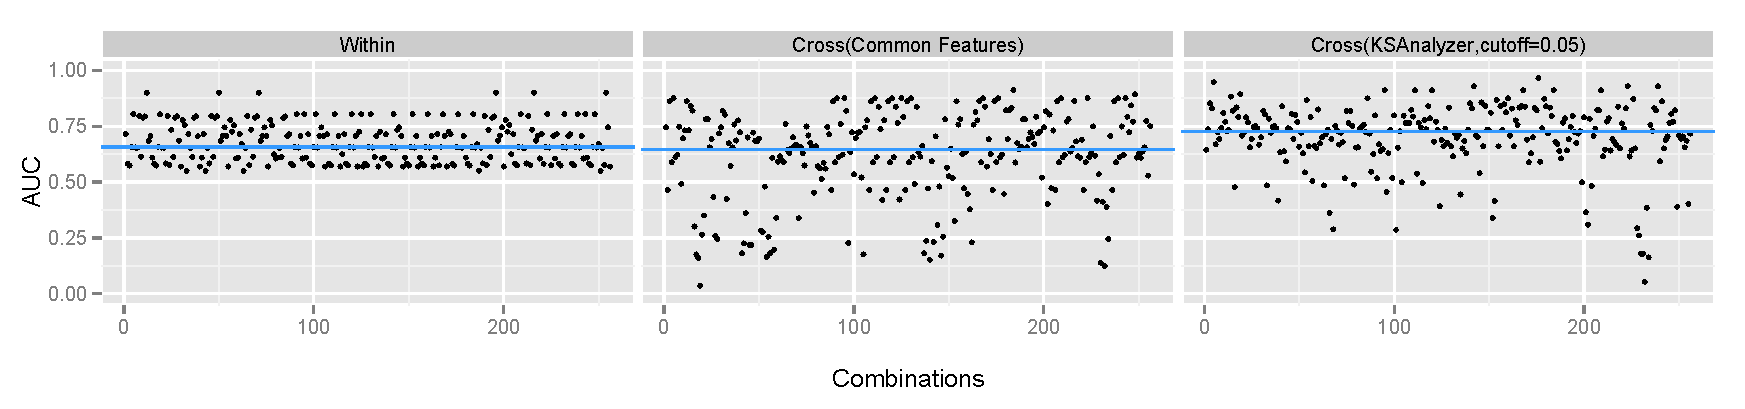
\includegraphics[width=\linewidth]{Figures/Result/auc_compare.pdf}
% 	\caption{Prediction performance comparison among within-results, cross-results
% 	by ASAnalyzer, random analyzer, and manual matching in terms of median AUC values.}
% 	\label{fig:compare_results_on_defect}
% \end{figure*}
% 
% In addition, the median AUC value of all predictions using all defect source
% groups (Defect All in Table~\ref{tab:compare}) is
% 0.701, which is a promising result since the median AUC values in
% within-predictions and cross-predictions by random analyzer and manual matching
% are 0.676, 0.599, and 0.609, respectively. In the case of AEEEM, the median AUC
% of manual feature matching is fairly high (0.673). However, the median AUC of
% within-prediction (0.675) outperforms that of manual feature matching with
% statistical significance (p=0.000).
% 
% Figure~\ref{fig:compare_results_on_defect} shows how each prediction performance
% of within- and cross-predictions varies. The solid line in
% Figure~\ref{fig:compare_results_on_defect} represents the overall prediction
% performance and the mean of all the median AUC values of the targets. Comparing
% the cross-results of AS to within-prediction results, we observed the
% cross-result is better than the within-result. We also compare cross-prediction
% results of AS, random analyzer, and manual matching as well. As we observe, the
% cross-result of AS outperforms that of both random analyzer and manual matching.
% 
% We conducted t-test (p<0.05) for those overall median AUC values between
% within-predictions and cross-predictions of AS. The cross-result of
% AS outperforms the within-result with statistical significance (p=0.002)
% and outperforms those of random analyzer and manual feature matching (p=0.000).
% Thus, we can confirm RQ2; cross-predictions by ASAnalyzer with the cutoff of
% 0.9 outperform to within-predictions in terms of median AUC in our
% experimental setting.


%\begin{result}
%Therefore, we can
%conclude that our cross-domain prediction model can predict defects in targets
%with high coverage
%\end{result}

%--------------------------------------------------------------
% \subsection{Within vs. Cross in non-defect$\Rightarrow$defect}
%--------------------------------------------------------------

% \begin{table}[t]
% \small
% \centering
% \caption{Average AUCs of Within and Cross-prediction results ASAnalyzer with
% Filters and Random Analyzer) by each
% source group in non-defect$\Rightarrow$defect.}
% \label{tab:compare_non_defect}
% \begin{tabular}{|c|c|c|c|c|}
% \hline
% 
% \multirow{2}{*}{\specialcell{{\bf Source}\\{\bf group}}}	&
% \multirow{2}{*}{{\bf Within}}	& \multicolumn{2}{c|}{{\bf Cross}}	&
% \multirow{2}{*}{\specialcell{{\bf Target}\\{\bf coverage}}}
% \\
% 
% \cline{3-4}
% 		& 	& \specialcell{{\bf ASw/F}} & {\bf Random} & \\ \hline
% 
% Effort & 0.63	& 0.84 & 0.73	& 11\% (3/28)\\ \hline
% Severity & N/A  & N/A	& N/A	& 0\% (0/28)\\ \hline
% {\bf SE all}  & {\bf0.63}	& {\bf 0.84} & {\bf 0.73}		& {\bf 11\%} (3/28)\\
% \hline \hline \hline
% Medical	& 0.69	& 0.71	& 0.58	& 32\% (9/28)\\ \hline
% Wine	& 0.57	& 0.55	& 0.57	& 4\% (1/28)\\ \hline \hline
% {\bf non-SE All} & {\bf 0.68}	& {\bf 0.70} & {\bf 0.58}	& {\bf 36\%} (10/28)\\
% \hline
% 
% %{\bf Non-defect All} &{\bf 0.67}	&{\bf 0.73}	&{\bf 0.61} &  \\ \hline
% \end{tabular}
% \end{table}

% Table~\ref{tab:compare_non_defect} shows cross-prediction results in
% non-defect$\Rightarrow$defect in terms of average AUC by each source group.
% Cross-results outperform within-results in non-defect$\Rightarrow$defect as
% well. We conducted the paired t-test for predictions in
% non-defect$\Rightarrow$defect. From the paired t-test, we could conclude that
% cross-results of ASAnalyzer with Filters were comparable to within-results.
% However, we observed very low prediction coverage; 3\% by SE and
% 36\% by non-SE. Thus, we may not generalize this observation, (In
% Section~\ref{sec:prediction_coverage}, we discuss prediction coverage in detail.)
% 
% Random analyzer in Effort in
% Table~\ref{tab:compare_non_defect} outperforms within-predictions in terms of
% average AUC. Note that its within-result is fairly low (0.63). In addition,
% Random analyzer result did not outperform the within-result with statistical significance
% (p=0.18).
% 
% 
% \begin{figure}[t]
% 	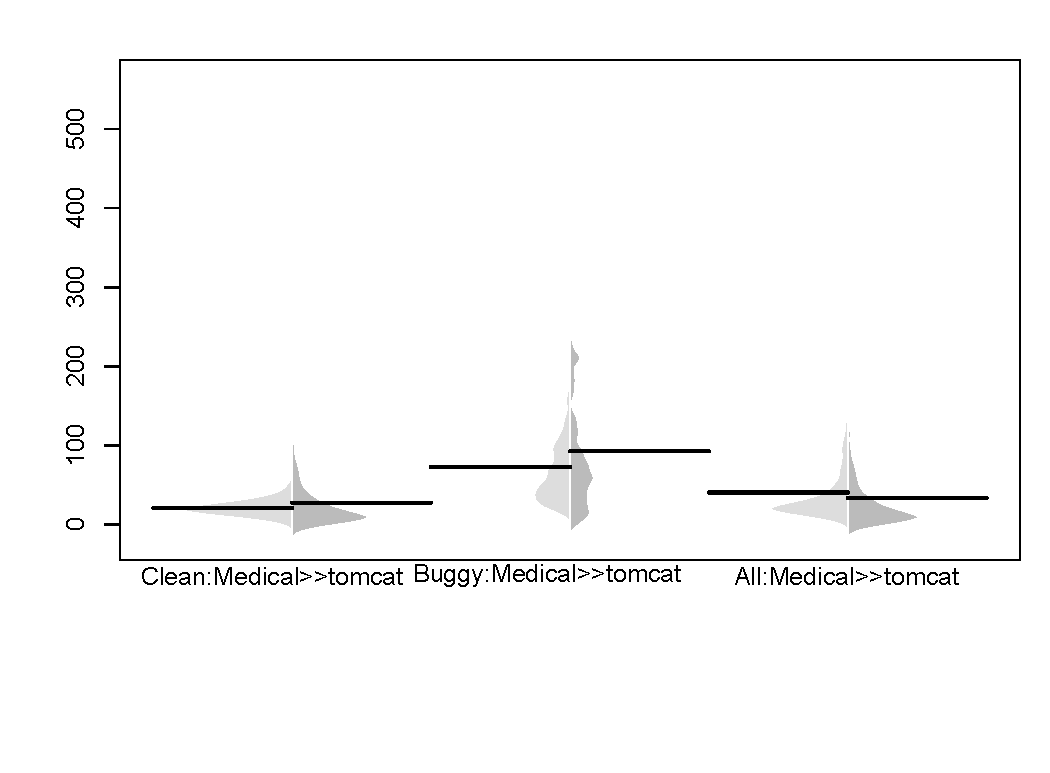
\includegraphics[width=\linewidth]{Figures/Result/medical_dist.pdf}
% 	\caption{Feature distribution of an matched feature from the prediction
% 	combination, Medical(area\_se)$\Rightarrow$Tomcat(rfc), of AUC=0.82.}
% 	\label{fig:medical_dist}
% \end{figure}
% 
% 
% We observed interesting results in Medical. Nine
% out of 28 targets in non-SE$\Rightarrow$defect predictions were covered by
% models from the Medical dataset. An example matched feature is standard error of
% nuclear area of cells (area\_se) of Medical and response for class
% (rfc, to measure coupling) of pc3 in NASA. The area\_se feature represents how
% much irregular the areas of cells are. The higher value of area\_se indicates the higher
% malignancy~\cite{Street93}. This characteristic of the feature, area\_se, is
% similar to that of typical features in defect datasets, as shown in
% Figure~\ref{fig:medical_dist}. We can clearly observe similar distribution
% between the matched features. In addition, original task of the Medical dataset
% was binary classification like software defect prediction in our experimental
% setting. This leads to a bit higher prediction coverage than SE datasets.
% 
% % However, models built by the Wine dataset covered only one target, ar1. This
% % poor coverage of Wine is also due to different characteristics of features from
% % that of typical features used in defect datasets.
% In Wine, ASAnalyzer with Filters is even worse than Random analyzer. In
% addition, models built by the Wine dataset covered only one target.
% Possible explanation is that features in Wine may have different characteristics
% from those in defect datasets and prediction task of Wine is multi-class
% classification rather than binary classification. This may lead
% to different results comparing to that of defect$\Rightarrow$defect.
% 
% For RQ2, we conducted paired t-test for non-defect$\Rightarrow$defect in terms
% of average AUC. Actually, cross-predictions were comparable to
% within-predictions with statistical significant (p=0.15). However, it is hard to
% generalize our result since prediction coverage is very low to conclude RQ2.

% \subsection{Prediction Coverage}
% \label{sec:prediction_coverage}
% 
% % Thus, we could confirm RQ1 in terms of
% % average AUC in our experimental setting. However, we could not confirm RQ3 since
% % prediction coverage of non-defect$\Rightarrow$defect predictions, were too low to compare results.
% 
% 
% \begin{table}[t]
% \small
% \centering
% \caption{Prediction Coverage of ASAnalyzer with Filters (cutoff>0.9) on
% defect$\Rightarrow$defect vs. non-defect$\Rightarrow$defect datasets in terms of
% average AUC.}
% \label{tab:prediction_coverage}
% %\setlength{\tabcolsep}{5pt}
% %\setlength{\extrarowheight}{1.5pt}
% \begin{tabular}{|c|@{ }c@{ }||@{ }c@{ }|@{ }c@{ }|}
% \hline
% \multirow{2}{*}{Target}	& \multirow{2}{*}{defect$\Rightarrow$defect} &
% \multicolumn{2}{c|}{non-defect$\Rightarrow$defect} \\ \cline{3-4}
% & 	& SE$\Rightarrow$defect &
% non-SE$\Rightarrow$defect \\\hline \hline
% EQ			&\cmark	&-&-	\\ \hline
% JDT			&\cmark	&-&\cmark	\\ \hline
% LC			&\cmark	&-&-\\ \hline
% ML			&\cmark	&-&-	\\ \hline
% PDE			&\cmark	&-&-	\\ \hline \hline
% 
% Apache		&\cmark	&-&-	\\ \hline
% Zxing		&\cmark	&-&\cmark	\\ \hline
% Safe		&\cmark	&-&\cmark\\ \hline \hline
% 
% ant-1.3		&\cmark	&-&-	\\ \hline
% arc			&\cmark	&-&-	\\ \hline
% camel-1.0	&\cmark	&-&-	\\ \hline
% poi-1.5		&\cmark	&-&-	\\ \hline
% redaktor	&\cmark	&-&-	\\ \hline
% skarbonka	&\cmark	&-&-	\\ \hline
% tomcat		&\cmark	&- &\cmark	\\ \hline
% velocity-1.4	&\cmark	&-&-	\\ \hline
% xalan-2.4	&\cmark	&-&-	\\ \hline
% xerces-1.2	&\cmark	&-&-	\\ \hline \hline
% 
% cm1			&\cmark	&-&\cmark	\\ \hline
% mw1			&\cmark	&\cmark&\cmark	\\ \hline
% pc1			&\cmark	&-&-	\\ \hline
% pc3			&\cmark	&-&-	\\ \hline
% pc4			&\cmark	&-&\cmark	\\ \hline \hline
% 
% ar1		&\cmark	&-&\cmark	\\ \hline
% ar3		&\cmark	&\cmark&\cmark	\\ \hline
% ar4		&\cmark	&-&\cmark	\\ \hline
% ar5		&\cmark	&\cmark&	\\ \hline
% ar6		&\cmark	&-&-	\\ \hline \hline
% Total & 28/28 (100\%) & 3/28 (11\%) & 10/28 (36\%) \\ \hline

% EQ	&12	&12	\\ \hline
% JDT	&14	&5	\\ \hline
% LC	&12	&11	\\ \hline
% ML	&16	&0	\\ \hline
% PDE	&13	&4	\\ \hline
% 
% Apache	&13	&4	\\ \hline
% Zxing	&20	&18	\\ \hline
% Safe	&17	&12	\\ \hline
% 
% ant-1.3	&9	&9	\\ \hline
% arc	&6	&5	\\ \hline
% camel-1.0	&9	&8	\\ \hline
% poi-1.5	&5	&2	\\ \hline
% redaktor	&10	&0	\\ \hline
% skarbonka	&11	&11	\\ \hline
% tomcat	&6	&4	\\ \hline
% velocity-1.4	&7	&1	\\ \hline
% xalan-2.4	&7	&1	\\ \hline
% xerces-1.2	&9	&0	\\ \hline
% 
% cm1	&17	&16	\\ \hline
% mw1	&9	&9	\\ \hline
% pc1	&14	&4	\\ \hline
% pc3	&12	&1	\\ \hline
% pc4	&15	&0	\\ \hline
% 
% ar1	&15	&15	\\ \hline
% ar3	&17	&16	\\ \hline
% ar4	&16	&16	\\ \hline
% ar5	&14	&12	\\ \hline
% ar6	&11	&10	\\ \hline \hline
% Total & 336 (28) & 206 (24) \\ \hline
% \end{tabular}
% \end{table}

% We checked prediction coverage of our framework for cross-domain defect
% prediction in detail. As shown in Table~\ref{tab:prediction_coverage}, all the
% targets in defect$\Rightarrow$defect could be predicted by our framework. This shows
% prediction coverage of our framework is 100\% in our experimental setting. To
% achieve 100\% coverage, there should exist matched features with high matching
% score ($>$0.9) and the prediction combinations should remain after applying LBM and DM filters. Thus,
% prediction coverage in defect$\Rightarrow$defect clearly shows that features of
% defect datasets could be transferred to build a prediction model and our
% framework could find matched features in defect$\Rightarrow$defect
% predictions.
% 
% However, non-defect$\Rightarrow$defect predictions lead to poor prediction
% coverage. In SE$\Rightarrow$defect prediction, three target projects, mw1, ar3,
% and ar5 are predicted by the framework. This low
% coverage is because of different characteristics of features between defect and
% non-defect datasets. Only three out of all combinations in SE$\Rightarrow$defect
% had co-occurrence features whose matching scores are higher than 0.9. In case
% of the Severity dataset, there were no matched features at all since features of
% the Severity dataset, created by text mining technique such as
% tf*idf~\cite{Menzies08}, are different from typical defect prediction features.


%This poor results in non-defect$\Rightarrow$defect predictions are obvious
% since datasets are collected in too different domains such as severity of
% issue reports and wine quality. We will discuss about this result more,
% particularly, ar5 in SE$\Rightarrow$defect in Section~\ref{sec:Discussion}.
% 
% Somebody may claim the high coverage of defect$\Rightarrow$defect is because of
% many source projects which can make more prediction combinations. In
% non-defect$\Rightarrow$defect predictions, we have few source projects (4)
% comparing to those (15-25) in defect$\Rightarrow$defect predictions for a
% target. However, before applying the HC filter, about 56\% of targets in average
% were already covered by each defect source dataset. This implies that we may
% cover all targets by two or three defect source datasets. In the same setting,
% average prediction coverage by SE and non-SE sources was about 5\% and 18\% respectively.
% 
% In our experimental settings, we could conclude about RQ3:
% \squishlist
% 	\item Our framework for
% cross-domain defect prediction could achieve 100\% prediction coverage in
% defect$\Rightarrow$defect predictions.
% 	\item Non-defect$\Rightarrow$defect predictions are hard to achieve good
% 	prediction coverage since features from different areas are most likely
% 	different from typical features of defect datasets. However, if there exist
% 	datasets whose feature characteristic is similar to that of typical features
% 	from defect datasets and prediction task is similar,i.e. binary classification,
% 	we can increase prediction coverage.
% \squishend
% 
% Due to the low prediction coverage of non-defect$\Rightarrow$defect, we
% only report detailed prediction results of defect$\Rightarrow$defect in
% next sub-sections.


\subsection{Win/Tie/Loss Results}

\begin{table}[!t]
%\small
\scriptsize
\centering
\caption{Win/Tie/Loss results of HDP by KSAnalyzer (cutoff=0.05)
against WPDP (Baseline1), CPDP-CM (Baseline2), and CPDP-IFS (Baseline3).}
\label{tab:win_results}
%\setlength{\tabcolsep}{5pt}
%\setlength{\extrarowheight}{1.5pt}
%\begin{tabular}{|@{ }c@{ }||@{ }c@{ }|@{ }c@{ }|@{ }c@{ }||@{ }c@{ }|@{ }c@{
%}|@{ }c@{ }|}
\begin{tabular}{|@{ }c@{}||@{ }c@{ }|@{ }c@{ }|@{ }c@{}||@{ }c@{ }|@{ }c@{
}|@{ }c@{}||@{ }c@{ }|@{ }c@{ }|@{ }c@{}|}
\hline

\multirow{3}{*}{{\bf Target}}
&\multicolumn{9}{c|}{\bf Against}
\\ \cline{2-10}
&\multicolumn{3}{c||}{\specialcell{{\bf WPDP}\\{(Baseline1)}}}
&\multicolumn{3}{c||}{\specialcell{{\bf CPDP-CM}\\{(Baseline2)}}}
&\multicolumn{3}{c|}{\specialcell{{\bf CPDP-IFS}\\{(Baseline3)}}}
\\
\cline{2-10}

& Win & Tie & Loss & Win & Tie & Loss & Win & Tie & Loss \\ \hline \hline

EQ			&4	&0	&0 & 2 & 2 & 0 &4 &0 &0 	\\ \hline
JDT			&0	&0	&5 & 3 & 0 & 2 &5 &0 &0	\\ \hline
LC			&6	&0	&1 & 3 & 3 & 1 &3 &1 &3	\\ \hline
ML			&0	&0	&6 & 4 & 2 & 0 &6 &0 &0	\\ \hline
PDE			&3	&0	&2 & 2 & 0 & 3 &5 &0 &0	\\ \hline \hline

Apache		&6	&0	&5 & 8 & 1 & 2 &9 &0 &2	\\ \hline
Safe		&14	&0	&3 & 12 & 0 & 5 &15 &0 &2	\\ \hline
Zxing		&8	&0	&0 & 6 & 0 & 2 &7 &0 &1	\\ \hline \hline

ant-1.3		&6	&0	&1 & 6 & 0 & 1 &5 &0 &2 \\ \hline
arc			&3	&1	&0 & 3 & 0 & 1 &4 &0 &0 \\ \hline
camel-1.0	&3	&0	&2 & 3 & 0 & 2 &4 &0 &1 \\ \hline
poi-1.5		&2	&0	&2 & 3 & 0 & 1 &2 &0 &2 \\ \hline
redaktor	&0	&0	&4 & 2 & 0 & 2	&3 &0 &1 \\ \hline
skarbonka	&11	&0	&0 & 4 & 0 & 7 &9 &0 &2 \\ \hline
tomcat		&2	&0	&0 & 1 & 1 & 0 &2 &0 &0 \\ \hline
velocity-1.4	&0	&0	&3 & 0 & 0 & 3 &0 &0 &3 \\ \hline
xalan-2.4	&0	&0	&1 & 1 & 0 & 0 &1 &0 &0	\\ \hline
xerces-1.2	&0	&0	&3 & 3 & 0 & 0 &1 &0 &2	\\ \hline \hline

cm1			&7	&1	&2 & 8 & 0 & 2 &9 &0 &1	\\ \hline
mw1			&5	&0	&1 & 4 & 0 & 2 &4 &0 &2	\\ \hline
pc1			&1	&0	&5 & 5 & 0 & 1 &6 &0 &0	\\ \hline
pc3			&0	&0	&7 & 7 & 0 & 0 &7 &0 &0	\\ \hline
pc4			&0	&0	&7 & 2 & 0 & 5 &7 &0 &0	\\ \hline \hline

ar1		&14	&0	&1	& 14 & 0 & 1 &11 &0 &4 \\ \hline
ar3		&15	&0	&0	& 5 & 0 & 10 &10 &2 &3 \\ \hline
ar4		&16	&0	&0	& 14 & 1 & 1 &15 &0 &1 \\ \hline
ar5		&14	&0	&4	& 14 & 0 & 4 &16 &0 &2 \\ \hline
ar6		&7	&1	&7	& 8 & 4 & 3  &12 &0 &3 \\ \hline \hline
Total & \specialcell{{147}\\{66.2\%}} &\specialcell{{3}\\{1.4\%}}
&\specialcell{{72}\\{32.4\%}}
& \specialcell{{147}\\{66.2\%}} &\specialcell{{14}\\{6.3\%}}
&\specialcell{{61}\\{27.5\%}}
& \specialcell{{182}\\{82.0\%}} &\specialcell{{3}\\{1.3\%}}
&\specialcell{{37}\\{16.7\%}}
\\
\hline
\end{tabular}
\end{table}


To investigate our performance evaluation in detail, we report
the Win/Tie/Loss results of HDP by KSAnalyzer with the cutoff of 0.05 against
WPDP (Baseline1), CPDP-CM (Baseline2), and CPDP-IFS
(Baseline3) in Table~\ref{tab:win_results}.


KSAnalyzer with the cutoff of 0.05 conducted 222 out of 600 prediction
combinations since 378 combinations do not have any matched
metrics because of the cutoff threshold. In
Table~\ref{tab:win_results}, the target dataset, EQ, was predicted in four
prediction combinations and our approach, HDP, outperforms Baseline1 and
Baseline3 in the four combinations (i.e. 4 Wins). However, HDP outperforms
Baseline2 in only two combinations of the target, EQ (2 Wins). 


% \subsection{Matched features}
% In this section, we discuss matched features to investigate prediction
% performance on cross-domain defect prediction in detail.

% A reason why ASAnalyzer can predict defects pretty well on cross-domain
% settings is that most defect prediction metrics usually represent complexity of
% source code and its change; it tends to be more buggy when the complexity is
% higher.
Against Baseline1, the six targets such as EQ, Zxing, skarbonka, tomcat,
ar3, and ar4 have only Win results. In other words, defects in those six targets
could be predicted better by other source projects using HDP models by
KSAnalyzer compared to WPDP models.

However, the eight targets such as JDT, ML, redaktor, velocity-1.4, xalan-2.4,
xerces-1.2, pc3, and pc4 have no Wins at all against Baseline1. In
addition, other targets still have Losses even though they have Win or Tie
results.

Overall, the numbers of Win and
Tie results are 147 and 3 respectively out of all of the 222 prediction
combinations.
This means that about 67.6\% of prediction combinations by our HDP
models achieve better or comparable prediction performance than those in
WPDP.

The Win/Tie/Loss results against Baseline2 and Baseline3 show a similar trend.
The HDP results in the 161 (72.5\%) out of 222 prediction combinations show
HDP outperforms and is comparable to CPDP-CM. Against Baseline3, 185
(83.3\%) predction combinations are Win or Tie results.

The Win/Tie/Loss results show that with our HDP model by
KSAnalyzer there is a higher possibility of getting a better prediction
performance.

However, there are still about 32\% Loss results against WPDP. In
Section~\ref{sec:Discussion}, we discuss and analyze why Loss results happen.


% In the SOFTLAB group, all projects get Win results
% which represent that average AUC of cross-prediction results outperform
% within-prediction results with statistical significance (the paired t-test,
% p=0.05).
% 
% There is one Tie result in cm1 of the NASA group. The Tie represents that
% a cross-prediction result is comparable to a within-prediction result with
% statistical significance. Overall, Win (17) and Tie (1) results are 18 out of 28
% predictions. Comparing to Loss results, many cross-predictions (64\%) have
% better or comparable results to within-predictions. In terms of Loss
% results, 10 predictions did not outperform within-results. 
%Even though some
% predictions have Loss results, their within-prediction results are already high
% and cross-prediction results are also pretty good, i.e. pc3 (0.76) and pc4(0.76) in NASA.
% In Section~\ref{sec:Discussion}, we will discuss why some predictions got Loss
% results in detail.

% \begin{table}[t]
% \small
% \centering
% \caption{Win/Tie/Loss results of cross-predictions against within-predictions
% in terms of average AUC.}
% \label{tab:win_results}
% %\setlength{\tabcolsep}{5pt}
% %\setlength{\extrarowheight}{1.5pt}
% \begin{tabular}{|@{ }c@{ }|@{ }c@{ }|@{ }c@{ }|@{ }c@{ }|@{ }c@{ }|}
% \hline
% Group 	& Target	& Within AUC	& Cross AUC & Result \\\hline
% \hline
% \multirow{4}{*}{AEEEM} & EQ			& 0.58	& 0.77	& Win	\\ \cline{2-5}
% & JDT			& 0.79	& 0.82	& Win	\\ \cline{2-5}
% & LC			& 0.57	& 0.79	& Win	\\ \cline{2-5}
% & ML			& 0.73	& 0.53	& Loss	\\ \cline{2-5}
% & PDE			& 0.68	& 0.67	& Loss	\\ \hline \hline
% 
% \multirow{3}{*}{ReLink} &Apache		& 0.71	& 0.68 	& Loss	\\ \cline{2-5}
% & Zxing		& 0.60	& 0.62	& Win	\\ \cline{2-5}
% & Safe		& 0.70	& 0.87	& Win	\\ \hline \hline
% 
% \multirow{10}{*}{MORPH} &ant-1.3		& 0.61	& 0.83	& Win	\\ \cline{2-5}
% & arc			& 0.66	& 0.79	& Win	\\ \cline{2-5}
% & camel-1.0	& 0.53	& 0.64	& Win	\\ \cline{2-5}
% & poi-1.5		& 0.70	& 0.73 	& Win	\\ \cline{2-5}
% & redaktor	& 0.74	& 0.45	& Loss	\\ \cline{2-5}
% & skarbonka	& 0.56	& 0.73	& Win	\\ \cline{2-5}
% & tomcat		& 0.78	& 0.79 	& Win	\\ \cline{2-5}
% & velocity-1.4	& 0.72	& 0.56	& Loss	\\ \cline{2-5}
% & xalan-2.4	& 0.75	& 0.68	& Loss	\\ \cline{2-5}
% & xerces-1.2	& 0.62	& 0.55	& Loss	\\ \hline \hline
% 
% \multirow{5}{*}{NASA} &cm1			& 0.63	& 0.64	& Tie	\\ \cline{2-5}
% & mw1			& 0.60	& 0.72	& Win	\\ \cline{2-5}
% & pc1			& 0.78	& 0.68	& Loss	\\ \cline{2-5}
% & pc3			& 0.79	& 0.76	& Loss	\\ \cline{2-5}
% & pc4			& 0.9	& 0.76	& Loss	\\ \hline \hline
% 
% \multirow{5}{*}{SOFTLAB} & ar1			& 0.57	& 0.73	& Win	\\ \cline{2-5}
% & ar3			& 0.55	& 0.84	& Win	\\ \cline{2-5}
% & ar4			& 0.64	& 0.82	& Win	\\ \cline{2-5}
% & ar5			& 0.75	& 0.93	& Win	\\ \cline{2-5}
% & ar6			& 0.64	& 0.74	& Win	\\ \hline \hline
% \multicolumn{5}{c}{Win: 17, Tie: 1, Loss: 10} \\ \hline

\section{Result in F-measure}
In this section, we evaluate HDP models in terms of f-measure. F-measure is one of the widely used measures to evaluate defect prediction models. Since f-measure is a harmonic mean of precision and recall, it provides actual prediction accuracy~\cite{Lee11,Rahman13,Fukushima14,Herzig13,Jing14}. Precision is the rate of correctly predicted buggy instances from instances predicted as buggy. Recall is the rate of correctly predicted buggy instances among all buggy instances.

To compute f-measure, we need to set the threshold of prediction probability~\cite{Lessmann08,Rahman12}. When a prediction model classifies an instance, the model usually provides prediction probability for the instance. For example, Instance A gets the prediction probability of 0.78 while Instance B gets the probability of 0.45 by the model. If we let the model predicts an instance as buggy when the probability is greater than `0.5', Instance A will be predicted as buggy (0.78$>$0.50) but Instance B will be predicted as clean (0.45$<$0.50). Here, the cutoff value of `0.5' that decides the bug-proneness of an instance is the threshold of prediction probability of the model. In most defect prediction literature, the widely used prediction threshold is 0.5~\cite{Lee11,Rahman13,Herzig13,Zimmermann09}. By changing the threshold, prediction results vary.

However, we cannot identify the optimal threshold to lead to the best prediction results in advance. To our knowledge, there are no existing approaches to identify the optimal threshold in advance. Some researchers analyze ROC curves but ROC curves can be drawn from past prediction histories~\cite{Fawcett06,Tosun09}. Without the past prediction histories, identifying the probability threshold is a challenging issue.

To identify the optimal threshold, we used information from the best threshold of a source dataset. After metric matching for HPD models, we can get a training set and build a HDP model. From this model, we can identify the best threshold of prediction probability for the training set itself. By using the best threshold from the training set and its model, we used the following three methods from the training set to decide the best threshold for the test set:
\squishlist
\item Using the best threshold value from the training set (BTHD)
\item Using the percentile rank of the best threshold among all threshold values (PRBTHD)
\item Using PRBTHD after filtering out prediction combinations whose threshold distributions between the training and test sets are not similar by the KS test with p$<$0.05 (PRBTHD\_KS).
\squishend

BTHD simply reuses the best threshold value from the training set for the test set. For example, if the HDP model built using the training set leads to the best f-measure on the training set itself with the threshold of 0.43, the prediction performance for the test set is computed by using the threshold of 0.43 as well.

To decide the best threshold for the test set, PRBTHD uses the percentile rank of the best threshold value among threshold values from the training set. If the percentile rank of the threshold of 0.43 is 64.2\%, PRBTHD find the threshold value whose percentile rank is 64.2\% or the nearest among threshold values from the test set. Since metric matching of HDP is based on similar distributions between source and target datsets, we assume that distributions of threshold values between the training and test sets should be similar. In other words, we design PRBTHD

\begin{table}[t]
%\small
\scriptsize
\centering
\caption{Median f-measure of HDP in KSAnalyzer (cutoff=0.05) in different threshold methods.
}
\label{tab:threshold_result}
\begin{tabular}{|c||c||c|c|c||c|}
%\begin{tabular}{|c|D||D|D|D||c|}
\hline

% \multirow{2}{*}{\specialcell{{\bf Source}\\{\bf group}}}	&
% \multirow{2}{*}{{\bf Within}} &
% \multicolumn{3}{c|}{{\bf Cross}}	&
% \multirow{2}{*}{\specialcell{{\bf Target}\\{\bf coverage}}}
\specialcell{{\bf Threshold}\\{\bf Methods}}
& {\bf F-measure}
& {\bf Win}\%
& {\bf Tie}\% 
& {\bf Loss}\%
& \specialcell{{\bf \# of}\\{\bf Predictions}} \\ \hline \hline
THD\_0.5 & 0.227	& 28.8\% & 4.1\%	& 67.1\% & 222\\ \hline
BTHD & 0.315	& 44.6\% & 5.9\%	& 49.5\% & 222\\ \hline
PRBTHD & 0.323	& 48.2\% & 5.4\%	& 46.4\% & 222\\ \hline
PRBTHD\_KS& 0.340	& 50.0\% & 10.3\%	& 39.7\% & 184\\ \hline
% 29\\
% \hline\hline
%\bf{\emph{All}} &  0.657 & 0.636 & \underline{\bf 0.724} & 100\%\\	%& 316\\
%\hline

%{\bf Non-defect All} &{\bf 0.67}	&{\bf 0.73}	&{\bf 0.61} &  \\ \hline


\end{tabular}
\end{table}

%The performance of a prediction model in terms of precision and recall is decided by the prediction probability of each prediction result of an instance. The prediction probability threshold of 0.5 is commonly used in literature~\jc{need citations}. However, the optimal threshold may be different and is difficult to identify in advance. To address this issue, we reuse the optimal threshold from the source used to build HDP models for the target. We design our empirical study to compare prediction results using the optimal threshold to those using the commonly used threshold, 0.5, in Section~\ref{sec:Evaluation}.

%To get the optimal threshold from the source, we compute all f-measures when a increasing threshold value changes prediction results.


%\begin{figure*}[t!]
	\renewcommand{\baselinestretch}{0.8}\begin{center}
		{\scriptsize
			\begin{tabular}{c|l|p{4.7in}}
				amc & average method complexity & e.g. number of JAVA byte codes\\\hline
				avg\, cc & average McCabe & average McCabe's cyclomatic complexity seen
				in class\\\hline
				ca & afferent couplings & how many other classes use the specific
				class. \\\hline
				class. \\\hline
				cam & cohesion amongst classes & summation of number of different
				types of method parameters in every method divided by a multiplication
				of number of different method parameter types in whole class and
				number of methods. \\\hline
				cbm &coupling between methods &  total number of new/redefined methods
				to which all the inherited methods are coupled\\\hline
				cbo & coupling between objects & increased when the methods of one
				class access services of another.\\\hline
				ce & efferent couplings & how many other classes is used by the
				specific class. \\\hline
				dam & data access & ratio of the number of private (protected)
				attributes to the total number of attributes\\\hline
				dit & depth of inheritance tree &\\\hline
				ic & inheritance coupling &  number of parent classes to which a given
				class is coupled (includes counts of methods and variables inherited)
				\\\hline
				lcom & lack of cohesion in methods &number of pairs of methods that do
				not share a reference to an case variable.\\\hline
				locm3 & another lack of cohesion measure & if $m,a$ are  the number of
				$methods,attributes$
				in a class number and $\mu(a)$  is the number of methods accessing an
				attribute, 
				then
				$lcom3=((\frac{1}{a} \sum, j^a \mu(a, j)) - m)/ (1-m)$.
				\\\hline
				loc & lines of code &\\\hline
				max\, cc & maximum McCabe & maximum McCabe's cyclomatic complexity seen
				in class\\\hline
				mfa & functional abstraction & number of methods inherited by a class
				plus number of methods accessible by member methods of the
				class\\\hline
				moa &  aggregation &  count of the number of data declarations (class
				fields) whose types are user defined classes\\\hline
				noc &  number of children &\\\hline
				npm & number of public methods & \\\hline
				rfc & response for a class &number of  methods invoked in response to
				a message to the object.\\\hline
				wmc & weighted methods per class &\\\hline
				nDefects & raw defect counts & Numeric: number of defects found in post-release bug-tracking systems.\\
				defect & defects present? & Boolean: if {\em nDefects} $>0$ then {\em true} else {\em false}
			\end{tabular}
		}
	\end{center}
	\caption{OO measures used in our defect data sets.  Last lines, denote the dependent variables.}\label{fig:ck}
\end{figure*}


\newcommand{\tion}[1]{\S\ref{sect:#1}}
% \newcommand{\fig}[1]{Figure~\ref{fig:#1}}
\newcommand{\eq}[1]{Equation~\ref{eq:#1}}
% \newcommand{\bi}{\begin{itemize}}
% \newcommand{\ei}{\end{itemize}}

\section{Explaining Results of Size Limits for Effective Transfer Learning}\label{sect:xplain}
To assess the generality of the above results in Section~\ref{sec:sizelimit}, we need some background knowledge that knows when a few samples will (or will not)
be sufficient to build a defect predictor. Using some sampling theory, this section:
\bi
\item
Builds such a mathematical model;
\item Maps known aspects
of defect data  into that model;
\item Identifies what would need to change before the above results would no longer hold.
\ei
To start, we repeat the {\em lessons learned} above as well as what is {\em known about defect data sets}.
Next, we define a {\em maths model} which will be used in a {\em Monte Carlo simulation} to generate a log of how many samples are required
to find some signal. This log will be summarized via a {\em decision tree learner}.

\subsection{Set up}
\subsubsection{ Lessons from the above work}

The above results show
that a small number
of examples are sufficient to build a defect predictor, even when the data is being transferred from columns with other names.
In the following we will build a model computing the probability that $n$ training examples are sufficient to detect $e$\% defective modules.

In order to simplify the analysis, we will divide $n$ into
  $n<50, n<100, n<200,n\ge 200$ respectively (and note that $n  \ge 200$ is where the above
  results do not hold).

\subsubsection{Known about defect data sets}\label{sect:data}

Recent
results~\cite{Zhang2014,nam2015clami} show that, for defect data, good
predictors can be built via a {\em median chop} of
numeric project data;
i.e. they are divided into $b=2$ bins.

Other results~\cite{shepperd94}
show that defect prediction data containing dozens
of attributes, many of which are correlated
attributes. Hence, while a data set may have many dimensions, it only really ``needs'' a few
(and by ``need'' we mean that adding in unnecessary dimensions does not add to the accuracy
of defect predictors learned from this data).


Feature subset selection algorithms~\cite{Hall03} can  determine
which  dimensions are needed, and which can be ignored.
When applied to defect data~\cite{Menzies07},
we found that those data sets may only need  $d \in \{2,3\}$
dimensions.

Hence, in the following, we will pay particular attention to the ``typical'' region of
 $b=2, d \le 3$.

\subsubsection{A Maths Model}

Before writing down some maths, it is useful to start with some intuitions.
Accordingly, consider a chess board  containing small  piles of defects in some cells.
Like all chess boards, this one is  divided into a grid of $b^2$ cells (in standard chess, $b=8$ so the board has 64 cells).
Further, some cells of the chess board are blank while other cells are $e$\% covered
with that signal.

If we throw a small pebble at that chess board, then  the odds
of hitting a defects is $c \times p$ where:
\bi
\item $c$ is the probability of picking a particular cell;
\item $p$ is the probability that, once we arrive at that cell, we will find  the  signal in that cell.
\ei
With a few changes, this chess board model can be
used to represent the process of machine
learning. For example,
instead of a board with two
dimensions, data mining works on a ``chess board''
with $d$ dimensions: i.e. one for all the independent
variables collected from a project (which are ``needed'', as defined as \tion{data}).

Also,
instead of each dimension being divided into eight (like a chess board), it is common in data mining for SE~\cite{Menzies2014a}
to divide dimensions accroding to some {\em descritization policy}~\cite{lust08}.
Discretization converts a numeric variable with infinite range into a smaller number of  $b$ bins. Hence, the number of cells in a
hyper-dimensional chess board is $b^d$ and the probability of selecting any one cell is
\begin{equation}\label{eq:c}c=1/(b^d)=b^{-d}\end{equation}
Once we arrive at any cells, we will be in a region with $e$ percent errors.
What  is the probability $p$ that we will find those $e$ errors, given $n$ samples from the training data?
According to Voas and Miller~\cite{voas1995software},
if we see something at probability $e$, then we will miss it at probability $1-e$.
After $n$ attempts, the probability of missing it is $(1-e)^n$ so the probability of stumbling onto $e$ errors is:
\begin{equation}\label{eq:p}
p(e,n) = 1-(1-e)^n
\end{equation}
The premise of data mining is that in the data ``chess board'', some cells contain more of the signal than others. Hence, the 
distribution of the $e$ errors are ``skewed'' by some factor $k$. If $k=1$, then all the errors are evenly distributed over all cells.
But at all other values of $k$, some cells contain more errors than others, computed as follows:
    \bi
  \item $R_c$ is a random number $0\le R \le 1$, selected for each part of the space $c\in C$.
  \item $x_c$ is the proportion of errors in each part of $C$. \mbox{$x_c =  R_{c\in C}^k$}.
  \item We normalize $x_c$ to be some ratio $0 \le x_c \le 1$ as follows: $X= \sum_{c\in C} x_c$ then $x_c = x_c/X$
    \ei
    If  $e$ is the ratio of classes within a software project containing errors, then $E$ 
    is the expected value  of selecting a cell {\em and} that cell containing errors:
    \begin{equation}\label{eq:E}
     E   = \sum_{c\in C}c \times x_ce
    \end{equation}
    where $c$ comes from \eq{c} and $e$ is the ratio of classes in the training set with defects.


Using these equations, we can determine how many
training examples $n$ are required before $p(E,n)$, from 
\eq{p}, returns a value more than some reasonable
threshold $T$.  To make that determination, we call
$p(E,n)$ for increasing values of $n$ until $p \ge
T$ (for this paper, we used $T = 67\%$).

For completeness, it should be added  that the procedure of the above paragraph is an {\em upper bound} on the
number of examples needed to find a signal since it
assumes random sampling of a skewed distribution. In
practice, if a data mining algorithm is smart, then
it would {\em increase} the probability of finding
the target signal, thus {\em decreasing} how many samples are required.

\subsubsection{Monte Carlo Simulation}
    The above maths lets us define
    a  Monte Carlo simulation to assess the external validity of our results.
    1000 times, we picked $k,d,b,e$ values at random from:
    \bi
      \item $k \in \{1,2,3,4,5\}$;
  \item $d \in \{3,4,5,6,7\}$ dimensions;
  \item $b \in \{2,3,4,5,6,7\}$ bins; 
    \item $e\in \{0.1,0.2,0.3,0.4\}$
      \ei
      (These ranges were set using our experience with data mining, For example, our prior work shows in defect prediction data sets
      with 40 or more dimensions, that good predictors can be built using $d\le 7$ of those dimensions~\cite{Menzies07}.)
      
     1000 times,
     we increased $n$ until \eq{p} showed  $p$ passed our reasonable threshold.
     Next, we generated examples of what $n$ value was found using  $k,b,d,e$.
     
\begin{figure}
\renewcommand{\baselinestretch}{0.75}
\begin{alltt}\scriptsize 
     1	  dimensions = (1,2)
     2	  |   dimensions = 1
     3	  |   |   e \(\le\) 0.1
     4	  |   |   |   bins = (1,2,3) : \(n < 50\) 
     5	  |   |   |   bins > 3       : \(n < 100\) 
     6	  |   |   e > 0.1 : \(n < 50\)  
     7	  |   dimensions > 1
     8	  |   |   bins = (1,2,3)
     9	  |   |   |   e = 0.1 : \(n < 100\) 
    10	  |   |   |   e > 0.1 : \(n < 50\)  
    11	  |   |   bins > 3
    12	  |   |   |   bins = (4,5)
    13	  |   |   |   |   e = 0.1 : \(n < 200\) 
    14	  |   |   |   |   e > 0.1
    15	  |   |   |   |   |   e \(\le\) 0.2
    16	  |   |   |   |   |   |   bins = 4 : \(n < 100\) 
    17	  |   |   |   |   |   |   bins = 5 : \(n < 200\) 
    18	  |   |   |   |   |   e > 0.2      : \(n < 100\) 
    19	  |   |   |   bins > 5
    20	  |   |   |   |   e \(\le\) 0.2 : \(n \ge 200 \) 
    21	  |   |   |   |   e > 0.2 : \(n < 200\)
    22	  dimensions > 2
    23	  |   bins = (1,2)
    24	  |   |   dimensions = (3,4,5)
    25	  |   |   |   dimensions = 3
    26	  |   |   |   |   e \(\le\) 0.2 : \(n < 200\) 
    27	  |   |   |   |   e > 0.2 : \(n < 50\) 
    28	  |   |   |   dimensions = (4,5)
    29	  |   |   |   |   e = 0.1 : \(n < 200\) 
    30	  |   |   |   |   e > 0.1
    31	  |   |   |   |   |   dimensions = 4 : \(n < 100\) 
    32	  |   |   |   |   |   dimensions = 5
    33	  |   |   |   |   |   |   e \(\le\) 0.3 : \(n < 200\) 
    34	  |   |   |   |   |   |   e > 0.3 : \(n < 100\) 
    35	  |   |   dimensions > 5 : \(n \ge 200 \) 
    36	  |   bins > 2
    37	  |   |   dimensions = 3
    38	  |   |   |   bins = (3,4)
    39	  |   |   |   |   e \(\le\) 0.3
    40	  |   |   |   |   |   bins = 3
    41	  |   |   |   |   |   |   e = 0.1 : \(n \ge 200 \) 
    42	  |   |   |   |   |   |   e > 0.1 : \(n < 200\) 
    43	  |   |   |   |   |   bins = 4 : \(n \ge 200 \) 
    44	  |   |   |   |   e > 0.3 : \(n < 200\) 
    45	  |   |   |   bins > 4 : \(n \ge 200 \) 
    46	  |   |   dimensions > 3 : \(n \ge 200 \)
\end{alltt}
\caption{How many $n$ examples are required to be at least 67\%
likely to find defects occuring at probability $e$.}\label{fig:dtree}
\end{figure}
\subsubsection{Decision Tree Learning}

    These examples were given to a decision tree learner to determine what $n$ values are selected by different
    ranges of $\{k,b,d,e\}$. Decision tree learners seek an attribute range that, when used to split the data,
      simplifies the distribution of the dependent variable in each split.
      The decision tree learner is then called recursively on each split.
      To test the stability of the learned model, the learning is repeated ten times, each time using 90\% of the data from training and the rest
      for testing. The weighted average performance values for the learned decision tree were remarkably good:
      \bi
    \item False alarm rates = 2\%;
    \item F-measures (i.e. the harmonic mean of recall and precision) of 95\%
      \ei
\subsection{Results}

The resulting decision tree, shown in \fig{dtree}, defined regions where
building defect predictors would be very easy and much harder:
\bi
\item
Lines 2 to 6 discuss a very easy case. Here, we only need
one dimension to build defect predictors and,
for such simple data sets, 50 to 100 examples are enough for defect prediction.
\item
Lines 22, 36, 46 show a branch of the decision tree
where needs many dimensions that divide into many bins.
For such data sets, we require a larger number of samples to learn a predictor ($n \ge 200$).
\ei
The key part of \fig{dtree} is the ``typical'' region defined in \tion{data};
i.e.    $b=2, d \le 3$:
\bi
\item Lines 7 to 10 show one set of branches covering this ``typical'' region. Note
lines 9,10:  we need up to 100 examples when the defect signal is rare (10\%) but
far fewer when the signal occurs at $e>10$\%.
\item
Lines 22 to 27 show another set of branches in this ``typical region''. Note lines 26, 27:
we need up 50 to 200 examples.
\ei
\subsection{Summary}
Our experiments with transfer learning showed that 50 to 200 examples are needed for adequate
transfer of defect knowledge. If the reader doubts that this number is too small to be effective,
we note that:
\bi
\item Other researchers working with Logistic Regression~\cite{peduzzi1996simulation}
have reported that 10 ``events per decision variable'' are adequate for building models using that
data miner. For our defect data sets, in \fig{small_epv}, we repeated the analysis of~\cite{peduzzi1996simulation}
and found that considering 2 independent variable on average, there was little improvement after 100 examples with EPV = 10 (as would have been predicted by~\cite{peduzzi1996simulation}).
\item The maths of \tion{xplain} shows that this ``100 examples are enough'' is a feature of the kinds of
data being explored; specifically, how many dimensions are needed and how many bins are required when dividing
those dimensions.
\ei

\section{Discussion} 
\label{sec:Discussion}

% \subsection{Matched features}
% In this section, we discuss matched features to investigate prediction
% performance on cross-domain defect prediction in detail.
% 
% \begin{figure}[t]
% 	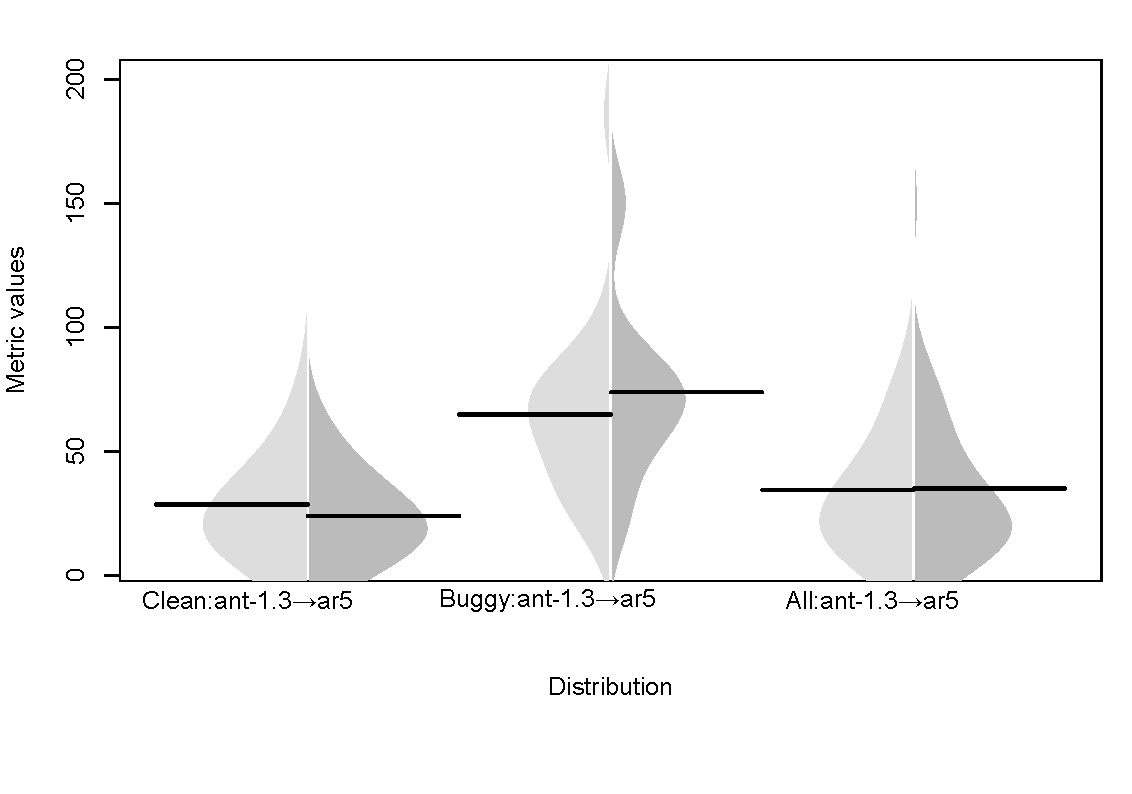
\includegraphics[width=\linewidth]{Figures/Result/best_dist.pdf}
% 	\caption{Feature value distribution of a matched feature from the
% 	prediction combination, ant-1.3$\Rightarrow$ar5, of AUC=0.938.}
% 	\label{fig:best_dist}
% \end{figure}
% 
% % A reason why ASAnalyzer can predict defects pretty well on cross-domain
% % settings is that most defect prediction metrics usually represent complexity of
% % source code and its change; it tends to be more buggy when the complexity is
% % higher.
% 
% In Figure~\ref{fig:best_dist}, we used beanplots~\cite{Beanplot08} to represent
% the feature value distribution of a matched feature in the prediction
% combination, ant-1.3$\Rightarrow$ar5, whose AUC is 0.938. The left side (light
% grey) of each beanplot shows distribution of buggy, clean, and all instances of
% source respectively, while the right side (dark grey) of each beanplot
% represents those of target. The horizontal black line represents an average
% value in each distribution. 
% 
% From Figure~\ref{fig:best_dist}, we can explain how ant-1.3$\Rightarrow$ar5 can
% have such a high AUC, 0.938. Suppose that a simple model predicts an instance as
% buggy when the feature value of the instance is more than 40 in case of
% Figure~\ref{fig:best_dist}. In both the source and target, approximately
% 70\% or more buggy and clean instances will be predicted correctly. In
% Figure~\ref{fig:best_dist}, the matched source and target features in
% ant-1.3$\Rightarrow$ar5 are the response for class (RFC: number of methods
% invoked by a class~\cite{Chidamber94}) and the number of unique operands
% (unique\_operands), respectively. The RFC and unique\_operands are not the same
% features. However, they have similar distribution as shown in
% Figure~\ref{fig:best_dist}. As we explained in Section~\ref{sec:Approach},
% typical defect prediction metrics (features) have a tendency that a higher
% complexity causes more buggy- proneness. The matched features
% follow this tendency very well so that the model using the matched features
% could achieve such a high AUC (0.938).
%but related; both features can be a factor contributing to how long and complex
% the source code is. In ar5, there is a more related feature such as comment\_loc. However, they are not actually matched since they have different distribution in terms of mean and standard deviation.

% \begin{figure}[t]
% 	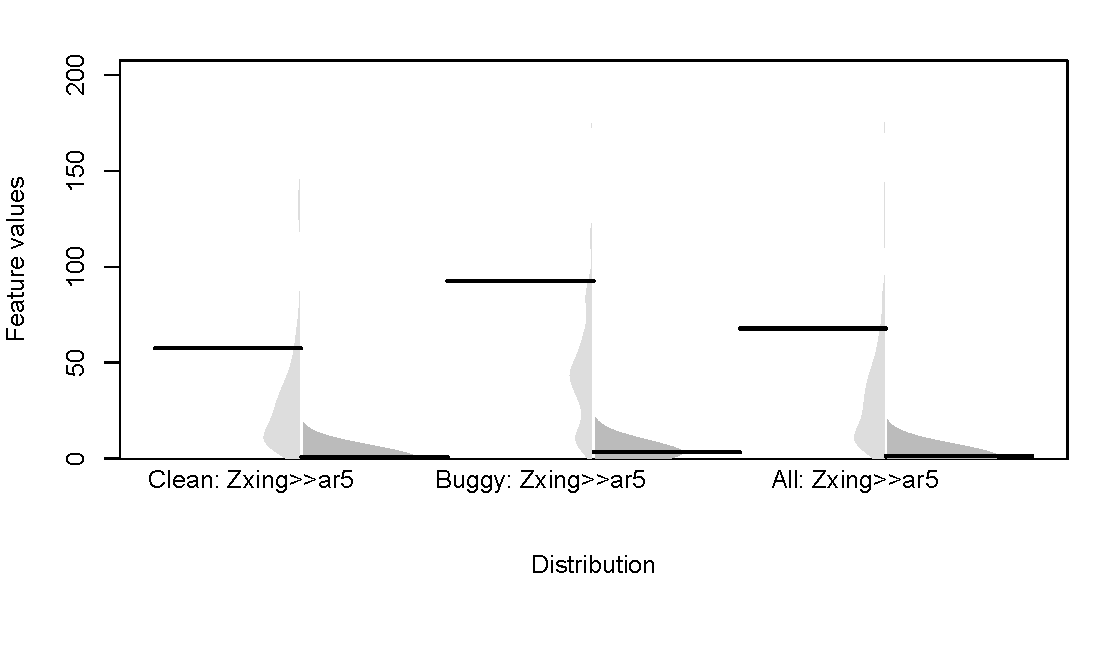
\includegraphics[width=\linewidth]{Figures/Result/beanplot_manual_matching.pdf}
% 	\caption{Feature value distribution of a manually matched feature (attribute)
% 	from the prediction combination, Zxing$\Rightarrow$ar5, of AUC=0.57.}
% 	\label{fig:manual_dist}
% \end{figure}
% 
% Each project
% may have different feature distributions even in projects with the same features
% since project characteristics can be made different by many other external
% environments such as the number of developers, product types, intended audiences, and so on.~\cite{Zimmermann09}.
% 
% Figure~\ref{fig:manual_dist} shows the feature value distribution of a
% manually matched feature of the prediction combination, Zxing$\Rightarrow$ar5, with AUC=0.57. The
% source and target features are CountLineCode and code-and-commend-loc
% respectively. Both features measure lines of code and comments, however their
% distributions are too different as seen in Figure~\ref{fig:manual_dist}. This
% is why cross-project prediction on projects with the same feature space is
% still a challenging issue~\cite{He12, Turhan09,Zimmermann09}. Thus, we tried to
% match features, which have similar distribution in a mechanical way to compare
% statistical parameters such as mean and standard deviation and observed
% many better prediction (Win) performance results as shown in
% Table~\ref{tab:win_results}.






\subsection{Practical Guidelines for HDP}

We proposed the HDP models to enable defect prediction on software projects
by using training datasets from other projects even with heterogeneous metric sets.
When we have training datasets in the same project or in other
projects with the same metric set, we can simply conduct
WPDP or CPDP using recently proposed CPDP techniques
respectively~\cite{Canfora13,Ma12,Nam13,Panichella14,Ryu14,Ryu15}.
However, in practice, it might be that no training datasets for
both WPDP and CPDP exist. In this case, we can apply the HDP approach.

In Section~\ref{sec:Result} and Table~\ref{tab:other_analyzers}, we confirm
that HDP by KSAnalyzer with the cutoff of 0.05
outperforms WPDP and shows 100\% target coverage.
Since KSAnalyzer can match similar source and target metrics, we guide the use
of KSAnalyzer for HDP. In terms of the matching score cutoff threshold, there is a
trade-off between prediction performance and target coverage. Since a cutoff
of 0.05 that is the widely used level of statistical
significance~\cite{Corder09}, we can conduct HDP using KSAnalyzer with the
cutoff of 0.05. However, we observe some Loss results in our empirical study.
To minimize the percentage of Loss results, we can sacrifice the target coverage
by increasing the cutoff as Table~\ref{tab:other_analyzers} shows KSAnalyzer with
the cutoff of 0.90 led to 100\% Win results in feasible predictions against
WPDP.

% However, we also observed Loss results and figured out filtering out Loss cases
% is quite challenging. When the metrics in defect datasets did not follow the
% common bug-prone tendency, our proposed HDP approach might not work well. We
% have a plan to address this challenging issue as future work.
% 
% Until addressing the issue about Loss cases, we can use KSAnalyzer with higher
% cutoffs. This option setting can mitigate Loss cases as KSAnalyzer with the
% cutoff of 0.90 achieved 100\% Wins in our experimental setting. However, the
% target coverage is only 21\%. To achive the 100\% target coverage, we might
% need more source datasets that have metrics matched with target metrics under
% KSAnalyzer with the cutoff of 0.90.

% \subsection{The number of matched features}
% \begin{table}[t]
% \small
% \centering
% \caption{The average number of matched features for each analyzer with
% cutoffs of 0.00, 0.05 and 0.90, and common features.}
% \label{tab:numFeatures}
% \begin{tabular}{|c|c|c|c||c|}
% \hline
% 
% % \multirow{2}{*}{{\bf Target}} &\multicolumn{3}{c||}{{\bf Cross by ASF}}
% % &\multicolumn{3}{c|}{{\bf Cross by manual}} \\ \cline{2-7}
% %  &Min & Max & Avg. &Min & Max & Avg. \\
% \multirow{2}{*}{{\bf Analyzer}}	& \multicolumn{3}{c||}{\specialcell{\bf{Average
% Number of}\\ {\bf Matched Features}}} &
% \multirow{2}{*}{\specialcell{\bf{Average number of}\\ \bf{Common Features}}} \\
% \cline{2-4} & {\bf 0.00} & {\bf 0.05} & {\bf 0.90} & \\
% \hline \hline
% 
% PAnalyzer			&7 &6 &1 & \multirow{4}{*}{5} \\ \cline{1-4}
% KSAnalyzer	&4 &2 &1 & \\ \cline{1-4}
% SCoAnalyzer			&7 &7 &6 & \\ \cline{1-4}
% PiAnalyzer			&7 &7 &6 & \\ \hline
% \end{tabular}
% \end{table}
% 
% Table~\ref{tab:numFeatures} shows the average number of matched
% features in prediction combinations between source and target datasets in each
% analyzer with cutoffs, 0.00, 0.05, and 0.9, and common features.
% 
% In KSAnalyzere with the cutoff of 0.00, the average number of matched features
% is four that is smaller than that (7) of other analyzers. The reason is that all
% matched features in some prediction combinations have matching scores of 0.00 so
% that these cross-predictions could not be conducted since there is no
% matched features whose matching scores are greater than 0.00 in the final set
% of matched features.
% For example, all matching scores in pc4$\Rightarrow$tomcat are 0.00 by
% KSAnalyzer so that this cross-prediction could not be conducted.
% 
% The average number of matched features in PAnalyzer and
% KSAnalyzer with the cutoff of 0.90 is one. The reason why the average
% number of matched features decreases is that poorly matched features with low
% matching scores automatically excluded according to the cutoff value.
% Many prediction combinations were not conducted because matched features whose
% matching scores are greater than 0.90 did not exist. Only 95 and 11 out of 600
% prediction combinations could be conducted in PAnalyzer and KSAnalyzer with the
% cutoff of 0.90 respectively.
% 
% However, the average number of matched features in ScoAnalyzer and PiAnalyzer
% seldom change. This means that the matching scores are very high in most matched
% features. Thus, using ScoAnalyzer and PiAnalyzer to match features between
% source and target datasets may not be helpful to judge whether matched features
% are similar or not.

\subsection{Threats to Validity}

%The selection of subjects used in our experiment can
%	be a threat. 
%Although we used 28 datasets for the experiment, 
We cannot generalize our conclusions since 28 datasets for the experiments may
not be representative.
	However, we tried to select various datasets used in papers published
	in top software engineering
	venues~\cite{DAmbros12,Lessmann08,Nam13,Peters12,Turhan09,Wu11}. In addition,
	we used datasets from both open-source (AEEEM~\cite{DAmbros12,Nam13},
	ReLink~\cite{Wu11}, and MORPH~\cite{Peters12}) and proprietary projects
	(NASA~\cite{Lessmann08,Turhan09} and SOFTLAB~\cite{Turhan09}).

We evaluated our HDP models in AUC.
	AUC is known as a good measure for comparing different prediction
	models~\cite{Giger12,Lessmann08,Rahman12,Song11}. However, validating
	prediction models in terms of both precision and recall is also required in
	practice. To fairly compare WPDP and HDP models in precision
	and recall, we need to identify a proper threshold of prediction probability.
	Identifying the proper threshold is a challenging issue and remains as
	future work.

For RQ1, we computed matching scores using all
	source and target instances for each prediction combination.
	With that matching scores, we tested prediction models on a test set from the 50:50 random splits because of the WPDP models as explained in Section~\ref{sec:expdesign}.
	To conduct WPDP with all instances of a project dataset as a test set, we need a training dataset from the previous releases of the same project. However, the training dataset is not
	available for our subjects. This may lead to an issue on construct validity since the matching score computations are not based on actual target instances used in the 50:50 random sampling. To address this issue, we additionally conducted experiments with different sample sizes, i.e., 50, 100, 150, and 200 rather using all instances when computing matching scores for HDP in Section~\ref{sec:sizelimit}.
%	about HDP against CPDP-CM and CPDP-IFS by testing a prediction model on a
%	test set using all instances of a target dataset in each prediction
%	combination.
%	In this setting, the median AUC of HDP was 0.723 and the median AUCs of the corresponding results in CPDP-CM and CPDP-IFS were 0.636 and 0.555
%	respectively.
%	These results are similar to those from the 50:50 random splits in
%	Section~\ref{sec:Result}. In other words, as long as the bug-prone tendency of matched metrics is consistent, HDP yields
%	promising results.
	

% In Section~\ref{sec:Result}, we found that cross-domain defect prediction from
% defect to defect datasets outperformed within-predictions with a higher
% chance; the percentages of Win+Tie were about 74\% and 82\% in the average
% F-measure and AUC, respectively. This result shows the possibility to improve
% defect prediction performance by using other defect datasets with different feature spaces.
% 
% \TODO{Analysis on co-occurrent features} To investigate how cross-domain defect
% prediction can build better prediction models, we took a closer look at the co-occurrent features identified by the
% co-occurrence analyzer.
% 
% \TODO{Analysis on SE and non-SE datasets}
% 
% \TODO{Summary of extensive and large scale results on different machine
% learning algorithms and co-occurrence analyzers with different cutoff values}
% Table~\ref{tab:win_results_on_diffrent_analyzers_ml_algs} represents the best win/tie/loss F-measure and AUC results on different analyzers and machine
% learning algorithms in our experimental settings. Results varies by analyzers
% and algorithms.
% Overall, PcoAnalyzer and Random forest lead to the best results comparing to other
% results. For example,...
% 
% \begin{table}
% \centering
% \caption{Best Win/Tie/Loss buggy F-measure and AUC results on different
% co-occurrent analyzers and machine learning (ML) algorithms.}
% \label{tab:win_results_on_diffrent_analyzers_ml_algs}
% %\setlength{\tabcolsep}{5pt}
% %\setlength{\extrarowheight}{1.5pt}
% \begin{tabular}{|@{ }c@{ }|@{ }c@{ }||@{ }c@{ }|@{ }c@{ }|@{ }c@{ }|@{ }c@{
% }||@{ }c@{ }|@{ }c@{ }|@{ }c@{ }|@{ }c@{ }|}
% \hline
% 	\multirow{2}{*}{\textbf{Analyzer}}
% 	&\multirow{2}{*}{\textbf{ML}}
% 	&\multicolumn{4}{c||}{\textbf{F-measure}}
% 	&\multicolumn{4}{c|}{\textbf{AUC}}
% 	\\ \cline{3-10}
% 	
% 	&
% 	&\textbf{cutoff}
% 	&\textbf{W}
% 	&\textbf{T}
% 	&\textbf{L}
% 	&\textbf{cutoff}
% 	&\textbf{W}
% 	&\textbf{T}
% 	&\textbf{L}
% 	\\ \hline \hline
% 	
% 	\multirow{7}{*}{AsAnalyzer}
% 	& J48
% 	&	0.65
% 	&	129 & 38 & 112
% 	&	0.65
% 	&	162 & 64 & 53
% 	\\ \cline{2-10}
% 	
% 	
% 	& RF
% 	&	0.80
% 	&	136 & 33 & 110
% 	&	0.85
% 	&	136 & 76 & 67
% 	\\  \cline{2-10}
% 	
% 	
% 	& NB
% 	&	0.80
% 	&	33 & 48 & 208
% 	&	0.90
% 	&	22 & 88 & 169
% 	\\  \cline{2-10}
% 	
% 	& BN
% 	&	0.75
% 	&	46 & 24 & 209
% 	&	0.70
% 	&	57 & 83 & 139
% 	\\  \cline{2-10}
% 	
% 	& LR
% 	&	0.70
% 	&	91 & 48 & 140
% 	&	0.80
% 	&	47 & 80 & 152
% 	\\  \cline{2-10}
% 	
% 	& MP
% 	&	0.75
% 	&	124 & 38 & 117
% 	&	0.65
% 	&	100 & 77 & 102
% 	\\  \cline{2-10}
% 	
% 	& SVM
% 	&	0.65
% 	&	143 & 28 & 108
% 	&	0.80
% 	&	122 & 63 & 94
% 	\\  \hline
% 	
% 	\multirow{7}{*}{TAnalyzer}
% 	& J48
% 	&	0.00
% 	&	131 & 44 & 104
% 	&	0.00
% 	&	164 & 64 & 51
% 	\\ \cline{2-10}
% 	
% 	
% 	& RF
% 	&	0.00
% 	&	123 & 46 & 110
% 	&	0.00
% 	&	132 & 80 & 67
% 	\\  \cline{2-10}
% 	
% 	
% 	& NB
% 	&	0.00
% 	&	37 & 39 & 203
% 	&	0.95
% 	&	16 & 65 & 165
% 	\\  \cline{2-10}
% 	
% 	& BN
% 	&	0.95
% 	&	30 & 12 & 204
% 	&	0.00
% 	&	54 & 85 & 140
% 	\\  \cline{2-10}
% 	
% 	& LR
% 	&	0.00
% 	&	82 & 52 & 145
% 	&	0.95
% 	&	34 & 60 & 152
% 	\\  \cline{2-10}
% 	
% 	& MP
% 	&	0.00
% 	&	120 & 36 & 123
% 	&	0.35
% 	&	65 & 86 & 128
% 	\\  \cline{2-10}
% 	
% 	& SVM
% 	&	0.00
% 	&	152 & 27 & 100
% 	&	0.00
% 	&	122 & 61 & 96
% 	\\  \hline
% 	
% 	\multirow{7}{*}{PcoAnalyzer}
% 	& J48
% 	&	0.75
% 	&	138 & 40 & 101
% 	&	\bf{0.80}
% 	&	\bf{167} & \bf{70} & \bf{42}
% 	\\ \cline{2-10}
% 	
% 	
% 	& \bf{RF}
% 	&	\bf{0.80}
% 	&	\bf{133} & \bf{49} & \bf{97}
% 	&	0.35
% 	&	142 & 82 & 55
% 	\\  \cline{2-10}
% 	
% 	
% 	& NB
% 	&	0.95
% 	&	39 & 35 & 205
% 	&	0.90
% 	&	19 & 101 & 159
% 	\\  \cline{2-10}
% 	
% 	& BN
% 	&	0.95
% 	&	52 & 32 & 195
% 	&	0.85
% 	&	51 & 96 & 132
% 	\\  \cline{2-10}
% 	
% 	& LR
% 	&	0.45
% 	&	90 & 52 & 137
% 	&	0.90
% 	&	49 & 75 & 155
% 	\\  \cline{2-10}
% 	
% 	& MP
% 	&	0.00
% 	&	122 & 43 & 144
% 	&	0.80
% 	&	90 & 85 & 104
% 	\\  \cline{2-10}
% 	
% 	& SVM
% 	&	0.90
% 	&	142 & 36 & 101
% 	&	0.15
% 	&	128 & 59 & 92
% 	\\  \hline
% 	
% % 	\multirow{6}{*}{ScoAnalyzer}
% % 	& J48
% % 	&	0.x
% % 	&	18 & 0 & 8
% % 	&	0.x
% % 	&	18 & 0 & 8
% % 	\\ \cline{2-10}
% % 	
% % 	
% % 	& RF
% % 	&	0.x
% % 	&	18 & 0 & 8
% % 	&	0.x
% % 	&	18 & 0 & 8
% % 	\\  \cline{2-10}
% % 	
% % 	
% % 	& NB
% % 	&	0.x
% % 	&	18 & 0 & 8
% % 	&	0.x
% % 	&	18 & 0 & 8
% % 	\\  \cline{2-10}
% % 	
% % 	& BN
% % 	&	0.x
% % 	&	18 & 0 & 8
% % 	&	0.x
% % 	&	18 & 0 & 8
% % 	\\  \cline{2-10}
% % 	
% % 	& LR
% % 	&	0.x
% % 	&	18 & 0 & 8
% % 	&	0.x
% % 	&	18 & 0 & 8
% % 	\\  \cline{2-10}
% % 	
% % 	
% % 	& SVM
% % 	&	0.x
% % 	&	18 & 0 & 8
% % 	&	0.x
% % 	&	18 & 0 & 8
% % 	\\  \hline
% 	
% 	
% 	\multirow{7}{*}{PiAnalyzer}
% 	& J48
% 	&	0.95
% 	&	132 & 35 & 112
% 	&	0.95
% 	&	159 & 65 & 55
% 	\\ \cline{2-10}
% 	
% 	
% 	& RF
% 	&	0.95
% 	&	126 & 33 & 120
% 	&	0.95
% 	&	139 & 70 & 70
% 	\\  \cline{2-10}
% 	
% 	
% 	& NB
% 	&	0.95
% 	&	34 & 30 & 215
% 	&	0.95
% 	&	17 & 88 & 174
% 	\\  \cline{2-10}
% 	
% 	& BN
% 	&	0.95
% 	&	48 & 27 & 204
% 	&	0.95
% 	&	55 & 86 & 138
% 	\\  \cline{2-10}
% 	
% 	& LR
% 	&	0.95
% 	&	88 & 45 & 146
% 	&	0.95
% 	&	38 & 88 & 153
% 	\\  \cline{2-10}
% 	
% 	& MP
% 	&	0.90
% 	&	112 & 32 & 135
% 	&	0.95
% 	&	77 & 83 & 119
% 	\\  \cline{2-10}
% 	
% 	& SVM
% 	&	0.95
% 	&	133 & 31 & 115
% 	&	0.95
% 	&	115 & 59 & 105
% 	\\  \hline
% 
% \end{tabular}
% \end{table}



\section{Conclusion}
\label{sec:Conclusion}
%\sung{Overall the conclusion is weak and does not convey the excitement of your
% wonderful work + results. Think about it and rewrite it.}

Cross-project defect prediction cannot be conducted across projects
with heterogeneous metric sets. To address
this limitation, we proposed heterogeneous defect prediction (HDP) based on
metric matching using statistical analysis~\cite{Massey51}. Our empirical evaluation
showed the proposed HDP models are feasible and yield promising results.
% The result (0.725) of the cross-domain prediction
% model by KSAnlyzer with the cutoff of 0.05 outperformed that of
% within-prediction (0.657) and cross-prediction using common features (0.645) in
% terms of a median AUC with statistical significance.

% To the best of our knowledge, this is
% the first study to focus on issues on different feature spaces for cross-project
% defect prediction.

% In our empirical study, we observed cross-domain prediction is feasible and
% promising. The result (0.725) of the cross-domain prediction
% model by KSAnlyzer with the cutoff of 0.05 outperformed that of
% within-prediction (0.657) and cross-prediction using common features (0.645) in
% terms of a median AUC with statistical significance. In addition, 65.6\% and 67.6\% of prediction
% combinations by our approach have outperforming (Win) and comparable (Tie)
% results to within-prediction and cross-prediction using common features with
% statistical significance. The Loss results were only less than about 35\%.
% However, in
% non-defect$\Rightarrow$defect, prediction coverage was about 11\% (SE) and 36\%
% (non-SE). This poor coverage shows our framework can match related features in
% defect$\Rightarrow$defect predictions.

% Say more about the implications of your work. What we can do using this? What
% new research directions you will open. (Hint: Potentially all heterogeneous
% data from other projects (such as data in PROMISE) can be used for my new
% project. Of cause, it is not limited to only defect prediction, right?)

% However, we observed some prediction combinations by our approach were still
% worse than baselines because of noisy target features that do not follow the
% bug-prone tendency of a source feature. Identifying noisy target features is
% still a challenging issue.
% This remains as future work.

HDP is very promising as it permits potentially all heterogeneous datasets
of software projects to be used for defect prediction on new projects or
projects lacking in defect data.
In addition, it may not be limited to defect prediction. This technique can
potentially be applicable to all prediction and recommendation based approaches
for software engineering problems.
As future work, we will explore the feasibility of building various prediction
and recommendation models using heterogeneous datasets.


% We investigated the distribution of
% matched features on Win and Loss prediction results and observed that
% the distribution similarity of matched features is important to conduct
% cross-domain defect prediction. Loss prediction results are caused by



% In addition, we measure prediction performance in terms
% of AUC. Although AUC is a useful measure to compare different prediction
% models~\cite{Giger12,Lessmann08,Rahman12,Song11}, precision and recall should
% also be considered to use our cross-domain defect prediction models in practice.
% However, to fairly compare prediction models in terms of precision and recall,
% we should identify a proper threshold of prediction probability.
% This is another challenging issue, which we keep as future
% work.




% An example of a floating figure using the graphicx package.
% Note that \label must occur AFTER (or within) \caption.
% For figures, \caption should occur after the \includegraphics.
% Note that IEEEtran v1.7 and later has special internal code that
% is designed to preserve the operation of \label within \caption
% even when the captionsoff option is in effect. However, because
% of issues like this, it may be the safest practice to put all your
% \label just after \caption rather than within \caption{}.
%
% Reminder: the "draftcls" or "draftclsnofoot", not "draft", class
% option should be used if it is desired that the figures are to be
% displayed while in draft mode.
%
%\begin{figure}[!t]
%\centering
%\includegraphics[width=2.5in]{myfigure}
% where an .eps filename suffix will be assumed under latex, 
% and a .pdf suffix will be assumed for pdflatex; or what has been declared
% via \DeclareGraphicsExtensions.
%\caption{Simulation results for the network.}
%\label{fig_sim}
%\end{figure}

% Note that IEEE typically puts floats only at the top, even when this
% results in a large percentage of a column being occupied by floats.
% However, the Computer Society has been known to put floats at the bottom.


% An example of a double column floating figure using two subfigures.
% (The subfig.sty package must be loaded for this to work.)
% The subfigure \label commands are set within each subfloat command,
% and the \label for the overall figure must come after \caption.
% \hfil is used as a separator to get equal spacing.
% Watch out that the combined width of all the subfigures on a 
% line do not exceed the text width or a line break will occur.
%
%\begin{figure*}[!t]
%\centering
%\subfloat[Case I]{\includegraphics[width=2.5in]{box}%
%\label{fig_first_case}}
%\hfil
%\subfloat[Case II]{\includegraphics[width=2.5in]{box}%
%\label{fig_second_case}}
%\caption{Simulation results for the network.}
%\label{fig_sim}
%\end{figure*}
%
% Note that often IEEE papers with subfigures do not employ subfigure
% captions (using the optional argument to \subfloat[]), but instead will
% reference/describe all of them (a), (b), etc., within the main caption.
% Be aware that for subfig.sty to generate the (a), (b), etc., subfigure
% labels, the optional argument to \subfloat must be present. If a
% subcaption is not desired, just leave its contents blank,
% e.g., \subfloat[].


% An example of a floating table. Note that, for IEEE style tables, the
% \caption command should come BEFORE the table and, given that table
% captions serve much like titles, are usually capitalized except for words
% such as a, an, and, as, at, but, by, for, in, nor, of, on, or, the, to
% and up, which are usually not capitalized unless they are the first or
% last word of the caption. Table text will default to \footnotesize as
% IEEE normally uses this smaller font for tables.
% The \label must come after \caption as always.
%
%\begin{table}[!t]
%% increase table row spacing, adjust to taste
%\renewcommand{\arraystretch}{1.3}
% if using array.sty, it might be a good idea to tweak the value of
% \extrarowheight as needed to properly center the text within the cells
%\caption{An Example of a Table}
%\label{table_example}
%\centering
%% Some packages, such as MDW tools, offer better commands for making tables
%% than the plain LaTeX2e tabular which is used here.
%\begin{tabular}{|c||c|}
%\hline
%One & Two\\
%\hline
%Three & Four\\
%\hline
%\end{tabular}
%\end{table}


% Note that the IEEE does not put floats in the very first column
% - or typically anywhere on the first page for that matter. Also,
% in-text middle ("here") positioning is typically not used, but it
% is allowed and encouraged for Computer Society conferences (but
% not Computer Society journals). Most IEEE journals/conferences use
% top floats exclusively. 
% Note that, LaTeX2e, unlike IEEE journals/conferences, places
% footnotes above bottom floats. This can be corrected via the
% \fnbelowfloat command of the stfloats package.


% if have a single appendix:
%\appendix[Proof of the Zonklar Equations]
% or
%\appendix  % for no appendix heading
% do not use \section anymore after \appendix, only \section*
% is possibly needed

% use appendices with more than one appendix
% then use \section to start each appendix
% you must declare a \section before using any
% \subsection or using \label (\appendices by itself
% starts a section numbered zero.)
%


%\appendices
%\section{Proof of the First Zonklar Equation}
%Appendix one text goes here.

% you can choose not to have a title for an appendix
% if you want by leaving the argument blank
%\section{}
%Appendix two text goes here.


% use section* for acknowledgment
%\ifCLASSOPTIONcompsoc
  % The Computer Society usually uses the plural form
%  \section*{Acknowledgments}
%\else
  % regular IEEE prefers the singular form
%  \section*{Acknowledgment}
%\fi


%The authors would like to thank...


% Can use something like this to put references on a page
% by themselves when using endfloat and the captionsoff option.
\ifCLASSOPTIONcaptionsoff
  \newpage
\fi



% trigger a \newpage just before the given reference
% number - used to balance the columns on the last page
% adjust value as needed - may need to be readjusted if
% the document is modified later
%\IEEEtriggeratref{8}
% The "triggered" command can be changed if desired:
%\IEEEtriggercmd{\enlargethispage{-5in}}

% references section

% can use a bibliography generated by BibTeX as a .bbl file
% BibTeX documentation can be easily obtained at:
% http://www.ctan.org/tex-archive/biblio/bibtex/contrib/doc/
% The IEEEtran BibTeX style support page is at:
% http://www.michaelshell.org/tex/ieeetran/bibtex/
%\bibliographystyle{IEEEtran}
% argument is your BibTeX string definitions and bibliography database(s)
%\bibliography{IEEEabrv,../bib/paper}
%
% <OR> manually copy in the resultant .bbl file
% set second argument of \begin to the number of references
% (used to reserve space for the reference number labels box)
%\begin{thebibliography}{1}

%\bibitem{IEEEhowto:kopka}
%H.~Kopka and P.~W. Daly, \emph{A Guide to \LaTeX}, 3rd~ed.\hskip 1em plus
%  0.5em minus 0.4em\relax Harlow, England: Addison-Wesley, 1999.

%\end{thebibliography}

\bibliographystyle{IEEEtran}
\bibliography{IEEEabrv,ref,ref_raleigh}

% biography section
% 
% If you have an EPS/PDF photo (graphicx package needed) extra braces are
% needed around the contents of the optional argument to biography to prevent
% the LaTeX parser from getting confused when it sees the complicated
% \includegraphics command within an optional argument. (You could create
% your own custom macro containing the \includegraphics command to make things
% simpler here.)
%\begin{IEEEbiography}[{\includegraphics[width=1in,height=1.25in,clip,keepaspectratio]{mshell}}]{Michael Shell}
% or if you just want to reserve a space for a photo:

\begin{IEEEbiography}{Michael Shell}
Biography text here.
\end{IEEEbiography}

% if you will not have a photo at all:
\begin{IEEEbiographynophoto}{John Doe}
Biography text here.
\end{IEEEbiographynophoto}

% insert where needed to balance the two columns on the last page with
% biographies
%\newpage

\begin{IEEEbiographynophoto}{Jane Doe}
Biography text here.
\end{IEEEbiographynophoto}

% You can push biographies down or up by placing
% a \vfill before or after them. The appropriate
% use of \vfill depends on what kind of text is
% on the last page and whether or not the columns
% are being equalized.

%\vfill

% Can be used to pull up biographies so that the bottom of the last one
% is flush with the other column.
%\enlargethispage{-5in}



% that's all folks
\end{document}


